
\input{mth309_notes_header.tex}


\begin{document}

\tableofcontents

\newpage

\setcounter{page}{1}
%---------------------------
%  Part 
%---------------------------
\lecture{Systems of linear equations}


\underline{\bf Systems of linear equations}

\vskip 7mm

$$
\left\{
\begingroup % keep the change local
\setlength\arraycolsep{2pt}
\begin{matrix}
a_{11}x_{1} &  +  & a_{12}x_{2} & +  & {\dots} &  +  & a_{1n}x_{n} & =  & b_{1} \\
\dots &    & \dots &   & {\dots} &    &\dots &  & \dots \\
\dots &    & \dots &   & {\dots} &    &\dots &  & \dots \\
a_{m1}x_{1} &  +  & a_{m2}x_{2} & +  & {\dots} &  +  & a_{mn}x_{n} & =  & b_{m} \\
\end{matrix}
\endgroup
\right.
$$


\newpage





\underline{\bf Question:} How many solutions a system of linear equations can have?

\vskip 10mm

{\bf Example:} Systems of equations in 2 variables.

\vskip 4mm

\begin{flushright}
\begin{tikzpicture}[scale=1]
\node[anchor=north] at (0,4)
{$
\begin{cases}
x_{1} + x_{2} = 1 \\
x_{1} - x_{2} = 1 \\
\end{cases}
$};
\begin{scope}[xshift = 115mm]
\foreach \x in {-2,...,4}{
\draw[help lines] (\x, -2) -- (\x, 4);
\draw[help lines] (-2, \x) -- (4, \x);
}
\draw[->, line width = 2pt] (-2,0) -- (4,0);
\draw[->, line width = 2pt] (0,-2) -- (0,4);
\end{scope}
\end{tikzpicture}
\end{flushright}
 
 \vskip -5mm
 
\begin{flushright}
\begin{tikzpicture}[scale=1]
\node[anchor=north] at (0,4)
{$
\begin{cases}
x_{1} + x_{2} = 1 \\
x_{1} + x_{2} = 2 \\
\end{cases}
$};
\begin{scope}[xshift = 115mm]
\foreach \x in {-2,...,4}{
\draw[help lines] (\x, -2) -- (\x, 4);
\draw[help lines] (-2, \x) -- (4, \x);
}
\draw[->, line width = 2pt] (-2,0) -- (4,0);
\draw[->, line width = 2pt] (0,-2) -- (0,4);
\end{scope}
\end{tikzpicture}
\end{flushright}

\vskip -5mm

\begin{flushright}
\begin{tikzpicture}[scale=1]
\node[anchor=north] at (0,4)
{$
\begin{cases}
\phantom{2}x_{1} +\phantom{2}x_{2} = 1 \\
2x_{1} + 2x_{2} = 2 \\
\end{cases}
$};
\begin{scope}[xshift = 112mm]
\foreach \x in {-2,...,4}{
\draw[help lines] (\x, -2) -- (\x, 4);
\draw[help lines] (-2, \x) -- (4, \x);
}
\draw[->, line width = 2pt] (-2,0) -- (4,0);
\draw[->, line width = 2pt] (0,-2) -- (0,4);
\end{scope}
\end{tikzpicture}
\end{flushright}

\newpage

{\bf Example:} Systems of equations in 3 variables.

\vskip 4mm


\begin{tikzpicture}[scale=1]
\node[anchor=north] at (0,3)
{$
\begin{cases}
x_{1} + x_{2} +x_{3} = 1 \\
x_{1} - x_{2} + x_{3} = 1 \\
x_{1}  = 1 \\
\end{cases}
$};
\node[anchor=north] at (12.1,4)
{
\includegraphics[width=60mm]{three_planes1.pdf}
};
\end{tikzpicture}
 \ 
 
 \vskip -4mm
 
 \ 
\begin{tikzpicture}[scale=1]
\node[anchor=north] at (0,3)
{$
\begin{cases}
x_{1} + x_{2} +x_{3} = 1 \\
x_{1} - x_{2} + x_{3} = 1 \\
x_{1} - x_{2} + x_{3} = 6 \\
\end{cases}
$};
\node[anchor=north] at (12,4)
{
\includegraphics[width=60mm]{three_planes2.pdf}
};
\end{tikzpicture}
 \ 
 
 \vskip -4mm
 
 \ 
\begin{tikzpicture}[scale=1]
\node[anchor=north] at (0,3)
{$
\begin{cases}
x_{1} + \phantom{5}x_{2} +x_{3} = 1 \\
x_{1} - \phantom{5}x_{2} + x_{3} = 1 \\
x_{1} + 5x_{2} + x_{3} = 1 \\
\end{cases}
$};
\node[anchor=north] at (11.9,4)
{
\includegraphics[width=60mm]{three_planes3.pdf}
};
\end{tikzpicture}

\newpage

\underline{\bf In general:}

\vskip 3mm

A system of linear equations can have either
\bitem
\item no solutions\\[-4mm]
\item exactly one solution\\[-4mm]
\item infinitely many solutions
\eitem

\vskip 10mm

\begin{cbox}[Definition]
If as system of linear equations which has no solutions is called an \emph{inconsistent system}. 
Otherwise the system is \emph{consistent}.
\end{cbox}


\newpage



%---------------------------
%  Part 2
%---------------------------
\lecture{Matrices and elementary row operations}


\underline{\bf Next:}


% Gauss-Jordan elimination diagram
\begin{sframe}

\ 

\vskip  -10mm

\ 

\begin{center}
\underline{\bf How to solve a system of linear equations}
\end{center}

\vskip -10mm

\btikz
\node[anchor = base] at (0,0)
{\begin{minipage}{50mm}
{\color{red} system of equations}
\vskip 2mm

$
\begin{cases}
-x_{1} + 2x_{2} + 3x_{3} = 4 \\
2x_{1} +6x_{3} = 9 \\
4x_{1} - x_{2} -3x_{3} = 0 \\
\end{cases}
$
\end{minipage}
};


\node[anchor = base] at (0,-5.7)
{\begin{minipage}{50mm}
{\color{red} solutions}
\vskip 2mm
$
\begin{cases}
x_{1} = {\dots} \\
x_{2} = {\dots}\\
x_{3} = {\dots} \\
\end{cases}
$
\end{minipage}
};

\node[anchor = base] at (10,0)
{\begin{minipage}{50mm}
{\color{red} \ }
\vskip 6mm
$
\bbm[c]
\phantom{\text{\ \ matrix in reduced \ \ }} \\
\text{augmented}   \\
\text{matrix}  \\
 \\
\ebm
$
\end{minipage}
};

\node[anchor = base] at (10,-5.7)
{\begin{minipage}{50mm}
{\color{red} \ }
\vskip 6mm
$
\bbm[c]
\phantom{\text{\ \ matrix in reduced \ \ }} \\
\text{ matrix in reduced }   \\
\text{row echelon form}  \\
 \\
\ebm
$
\end{minipage}
};

\node[single arrow, draw,  minimum height = 35mm, minimum width = 22mm, 
single arrow head extend= 1mm,  single arrow tip angle = 120, text height=2ex, text depth=1ex, 
 line width = 2pt, red, text = red]  
at (5.0, -0.1) {\small \emph{\begin{tabular}{l} make  \\ a matrix \end{tabular}}}; 

\node[single arrow, draw,  minimum height = 60mm, minimum width = 22mm, 
single arrow head extend= 1mm,  single arrow tip angle = 120, text height=2ex, text depth=1ex, 
 line width = 2pt, red, text = red,  shape border rotate = 180]  
at (4.3, -5.8) {\small\emph{\begin{tabular}{l} read off  \\ solutions\end{tabular}}}; 


\node[single arrow, draw,  minimum height = 27mm, minimum width = 45mm, 
single arrow head extend= 1mm,  single arrow tip angle = 130, text height=2ex, text depth=1ex, 
 line width = 2pt, red, text = red,  shape border rotate = 270]  
at (10.45, -2.7) {\small\emph{\begin{tabular}{c}  \\ Gauss-Jordan \\ elimination\end{tabular}}}; 
\etikz
\end{sframe}



\newpage

\underline{\bf Matrices}

\vskip 5mm

matrix $=$ rectangular array of numbers


\vskip 10mm

{\bf Example.}

\vskip 5mm

$$
\bbm[rrrrrr]
1 & 2 & 3  \\
4 & 5 & 6  \\
\ebm
\ \ \ \ \ \ \ \ \ \ \ \ \ \ \ \ \ \ \ \ \ \ \ \ \ \ \ \ \ \ \ \ \ \ \ \ \  
\bbm[rrrrrr]
1 & 2 & 0  \\
7 & -5 & 1  \\
8 & 10 & 7  \\
6 & 4 & 3  \\
\ebm
$$




\vskip 30mm

\begin{cbox}[Note]
Every system of linear equations can be represented by a matrix.
\end{cbox}


\vskip 5mm

{\bf Example.}

\vskip 5mm

$
\begin{cases}
-x_{1} + 2x_{2} + 3x_{3}  = 4 \\
2x_{1} + 6x_{3} = 9 \\
4x_{1} -x_{2} -3x_{3} = 0 \\
\end{cases}
$


\newpage

\underline{\bf Elementary row operations:}

\vskip 10mm


{\bf 1) Interchange of two rows.}


\vskip 10mm

{\bf Example.}

\vskip 3mm

$
\bbm[rrrrr]
1 & 2 & 3 & 4  \\
0 & 1 & 5 & 1  \\
4 & 3 & 0 & 7  \\
\ebm
$

\vskip 25mm


{\bf 2) Multiplication of a row by a non-zero number.}

\vskip 10mm

{\bf Example.}

\vskip 3mm

$
\bbm[rrrrr]
1 & 2 & 3 & 4  \\
0 & 1 & 5 & 1  \\
4 & 3 & 0 & 7  \\
\ebm
$

\vskip 25mm

{\bf 3) Addition of a multiple of one row to another row.}

\vskip 10mm

{\bf Example.}

\vskip 3mm

$
\bbm[rrrrr]
1 & 2 & 3 & 4  \\
0 & 1 & 5 & 1  \\
4 & 3 & 0 & 7  \\
\ebm
$



\newpage

\begin{cbox}[Proposition]
Elementary row operations do not change solutions of the system of equations represented by a matrix. 
\end{cbox}

\btikz[line1/.style ={line width = 1.5pt}]
\draw[opacity = 0] (-2, 0) -- (15,0); % for picture positioning
\draw[line1] (0,0) rectangle +(5,2) node[pos=0.5] {\begin{tabular}{c} system of \\ linear equations \end{tabular}};
\draw[line1] (0,-5.5) rectangle +(5,2) node[pos=0.5] {\begin{tabular}{c} system of \\ linear equations \end{tabular}};
\draw[line1] (8,0) rectangle +(5,2) node[pos=0.5] {\begin{tabular}{c} augmented \\matrix \end{tabular}};
\draw[line1] (8,-5.5) rectangle +(5,2) node[pos=0.5] {\begin{tabular}{c} augmented \\ matrix \end{tabular}};

\node[anchor =  tail, single arrow, draw,  minimum height = 21mm, minimum width = 15mm, 
single arrow head extend= 1mm,  single arrow tip angle = 120, text height=2ex, text depth=1ex, 
 line width = 2pt, red, text = red]  
at (5.5, 1) {}; 

\node[anchor =  tip, single arrow, draw,  minimum height = 21mm, minimum width = 15mm, 
single arrow head extend= 1mm,  single arrow tip angle = 120, text height=2ex, text depth=1ex, 
 line width = 2pt, red, text = red, shape border rotate = 180]  
at (5.42, -4.5) {}; 

\node[anchor =  tail, single arrow, draw,  minimum height = 25mm, minimum width = 21mm, 
single arrow head extend= 0.5mm,  single arrow tip angle = 120, text height=2ex, text depth=1ex, 
 line width = 2pt, red, text = red, shape border rotate = 270]  
at (10.5, -0.5) {}; 

\node[anchor = center, red, fill= white] at (10.5, -1.5) {\small \begin{tabular}{c}elementary \\ row operation \end{tabular}};

\draw[shorten <= 20pt, shorten >= 20pt, <->, >={Triangle[length = 10pt, width = 12pt]}, line width = 4pt, red] (0, 1.25)  to[out = 210, in = 150] node[anchor = west]  {\small \begin{tabular}{l}different systems \\ same solutions \end{tabular}} (0, -4.75) ; 

\etikz



%---------------------------
%  Part 3
%---------------------------
\lecture{Gauss-Jordan elimination}


\underline{\bf Recall:}


% Gauss-Jordan elimination diagram
\begin{sframe}

\ 

\vskip  -10mm

\ 

\begin{center}
\underline{\bf How to solve a system of linear equations}
\end{center}

\vskip -10mm

\btikz
\node[anchor = base] at (0,0)
{\begin{minipage}{50mm}
{\color{red} system of equations}
\vskip 2mm

$
\begin{cases}
-x_{1} + 2x_{2} + 3x_{3} = 4 \\
2x_{1} +6x_{3} = 9 \\
4x_{1} - x_{2} -3x_{3} = 0 \\
\end{cases}
$
\end{minipage}
};


\node[anchor = base] at (0,-5.7)
{\begin{minipage}{50mm}
{\color{red} solutions}
\vskip 2mm
$
\begin{cases}
x_{1} = {\dots} \\
x_{2} = {\dots}\\
x_{3} = {\dots} \\
\end{cases}
$
\end{minipage}
};

\node[anchor = base] at (10,0)
{\begin{minipage}{50mm}
{\color{red} \ }
\vskip 6mm
$
\bbm[c]
\phantom{\text{\ \ matrix in reduced \ \ }} \\
\text{augmented}   \\
\text{matrix}  \\
 \\
\ebm
$
\end{minipage}
};

\node[anchor = base] at (10,-5.7)
{\begin{minipage}{50mm}
{\color{red} \ }
\vskip 6mm
$
\bbm[c]
\phantom{\text{\ \ matrix in reduced \ \ }} \\
\text{ matrix in reduced }   \\
\text{row echelon form}  \\
 \\
\ebm
$
\end{minipage}
};

\node[single arrow, draw,  minimum height = 35mm, minimum width = 22mm, 
single arrow head extend= 1mm,  single arrow tip angle = 120, text height=2ex, text depth=1ex, 
 line width = 2pt, red, text = red]  
at (5.0, -0.1) {\small \emph{\begin{tabular}{l} make  \\ a matrix \end{tabular}}}; 

\node[single arrow, draw,  minimum height = 60mm, minimum width = 22mm, 
single arrow head extend= 1mm,  single arrow tip angle = 120, text height=2ex, text depth=1ex, 
 line width = 2pt, red, text = red,  shape border rotate = 180]  
at (4.3, -5.8) {\small\emph{\begin{tabular}{l} read off  \\ solutions\end{tabular}}}; 


\node[single arrow, draw,  minimum height = 27mm, minimum width = 45mm, 
single arrow head extend= 1mm,  single arrow tip angle = 130, text height=2ex, text depth=1ex, 
 line width = 2pt, red, text = red,  shape border rotate = 270]  
at (10.45, -2.7) {\small\emph{\begin{tabular}{c}  \\ Gauss-Jordan \\ elimination\end{tabular}}}; 
\etikz
\end{sframe}


\vskip  5mm

\textbullet \ Every system of linear equations can be represented by a matrix


\vskip 5mm

\textbullet \ Elementary row operations:
\benu
\item[-] interchange of two rows \\[-4mm]
\item[-] multiplication of a row by a non-zero number\\[-4mm]
\item[-] addition of a multiple of one row to another row.
\eenu

\vskip 5mm

\textbullet \ Elementary row operations do not change solutions of systems of linear equations.










\newpage

\begin{cbox}[Definition]
A matrix is in the \emph{row echelon form} if:
\bitem
\item[\bf{1)}] the first non-zero entry of each row is a 1 (``a leading one'');
\item[\bf{2)}] the leading one in each row is to the right of the leading one in the row above it.
\eitem

\vskip 2mm

A matrix is in the \emph{reduced row echelon form} if in addition it satisfies:
\bitem
\item[\bf{3)}] all entries above each leading one are 0. 
\eitem
\end{cbox}





\vskip 30mm

$$
\bbm[r]
1 & \ast  & \phantom{-}\ast & \ast & 0 & 0 & \ast & \ast & 0 \\[1mm]
0 & 0  & 0 & 0 & 1 & 0 & \ast & \ast & 0 \\[1mm]
0 & 0  & 0 & 0 & 0 & 1 & \ast & \ast & 0 \\[1mm]
0 & 0  & 0 & 0 & 0 & 0 & 0 & 0 & 1 \\[1mm]
0 & 0  & 0 & 0 & 0 & 0 & 0 & 0 & 0 \\
\ebm
$$

\vskip 10mm 

($\ast = $ any number)


\vskip 10mm

{\bf Example}

$$
\bbm[rrrrrr]
1 & 0 & 4 &  0 & 7 & 0 \\
0 & 1 & 5 &  0 & 1 & 0 \\
0 & 0 & 0 &  1 & 3 & 0 \\
0 & 0 & 0 &  0 & 0 & 1 \\
\ebm
\ \ \ \ \ \ \ \ 
\bbm[rrrrrr]
1 &2 & 4 &   6 & 7 & 0 \\
0 & 1 & 5 &  0 & 1 & 2 \\
0 & 0 & 0 &  1 & 3 & 0 \\
0 & 0 & 0 &  0 & 0 & 0 \\
\ebm
\ \ \ \ \ \ \ \ 
\bbm[rrrrrr]
1 & 0 & 4 &  0 & 7 & 0 \\
0 & 0 & 1 &  0 & 1 & 0 \\
0 & 1 & 3 &  6 & 3 & 0 \\
0 & 0 & 0 &  0 & 0 & 1 \\
\ebm
$$

\newpage

\begin{cbox}[Fact]
If a system of linear equations is represented by a matrix in the reduced row echelon form then it is easy to solve the 
system.
\end{cbox}


\vskip 10mm

{\bf Example}

\vskip 10mm

$
\bbm[rrrr|r]
1 & \phantom{.}0 & \phantom{.}3 & \phantom{.}0\phantom{.} & \phantom{.}0 \\
0 & 1 & 7 &  0\phantom{.} & 0 \\
0 & 0 & 0 &  1\phantom{.} & 0 \\
0 & 0 & 0 &  0\phantom{.} & 1 \\
\ebm
$


\vskip 90mm

\begin{cbox}[Proposition]
A matrix in the reduced row echelon form represents an inconsistent system if and only if it contains a row 
of the form
$$
\bbm
0 & 0 & 0 & {\dots} & 0 & 1 \\ 
\ebm
$$
i.e. with the leading one in the last column.
\end{cbox}


\newpage


{\bf Example}

\vskip 10mm

$
\bbm[rrrr|r]
1 & \phantom{.}0 & \phantom{.}3 & \phantom{.}0\phantom{.} & \phantom{.}0 \\
0 & 1 & 7 &  0\phantom{.} & 0 \\
0 & 0 & 0 &  1\phantom{.} & 0 \\
0 & 0 & 0 &  0\phantom{.} & 0 \\
\ebm
$


\vskip 150mm

\begin{cbox}[Note]
In an augmented matrix in the reduced row echelon form free variables correspond to columns of the coefficient 
matrix that do not contain leading ones. 

\end{cbox}

\newpage


{\bf Example}

\vskip 10mm

$
\bbm[rrrr|r]
1 & \phantom{.}0 & \phantom{.}0 & \phantom{.}0\phantom{.} & \phantom{.}5 \\
0 & 1 & 0 &  0\phantom{.} & 6 \\
0 & 0 & 1 &  0\phantom{.} & 7 \\
0 & 0 & 0 &  1\phantom{.} & 8 \\
\ebm
$


\vskip 150mm

\begin{cbox}[Note]
A matrix in the reduced row echelon form represents a system of equations with exactly one solution if and only if 
it has a leading one in every column except for the last one.  

\end{cbox}


\newpage

\underline{\bf Gauss-Jordan elimination process (= row reduction)}

\ 

\vskip -20mm 

\ 

\btikz
\node[anchor = base] at (-1.5,0)
{\begin{minipage}{50mm}
{\color{red} \ }
\vskip 6mm
$
\bbm[c]
\phantom{\text{\ \ \ \ echelon form\ \ \ \ }} \\
\text{matrix}   \\
\text{\ }  \\
\ebm
$
\end{minipage}
};


\node[anchor = base] at (10.5, 0)
{\begin{minipage}{50mm}
{\color{red} \ }
\vskip 6mm
$
\bbm[c]
\text{matrix} \\
\text{in the reduced row} \\
\text{\ \ \ \ echelon form\ \ \ \ } \\
\ebm
$
\end{minipage}
};

\node[single arrow, draw,  minimum height = 35mm, minimum width = 22mm, 
single arrow head extend= 1mm,  single arrow tip angle = 120, text height=2ex, text depth=1ex, 
 line width = 2pt, red, text = red]  
at (4.5, -0.2) {\small \emph{\begin{tabular}{c} elementary  \\ row operations \end{tabular}}}; 
\etikz

\vskip 20mm

\benu
\item[\raisebox{-1ex}{\huge\ding{192}}] Interchange rows, if necessary, to bring a non-zero element to the top of the first non-zero 
column of the matrix. \\[6mm]

\item[\raisebox{-1ex}{\huge\ding{193}}] Multiply the first row so that its first non-zero entry becomes 1.   \\[6mm]

\item[\raisebox{-1ex}{\huge\ding{194}}]Add multiples of the first row to eliminate non-zero entries below 
the leading one.   \\[6mm]

\item[\raisebox{-1ex}{\huge\ding{195}}]Ignore the first row; apply steps 1-3 to the rest of the matrix. \\[6mm]

\item[\raisebox{-1ex}{\huge\ding{196}}] Eliminate non-zero entries above all leading ones.  \\[6mm]
\eenu

\newpage

{\bf Example.}

\vskip 5mm 

$
\bbm
0 & 4 & -8 & 0 & 4 \\
2 & 6 & -6 & -2 & -4 \\
2 & 7 & -8 & 0 & -1 \\
\ebm
$


\newpage

\begin{center}
\underline{\bf How to solve systems of linear equations: example}
\end{center}

\vskip 5mm 

$
\begin{cases}
4x_{2} - 8x_{3} = 4 \\
2x_{1} +6x_{2} -6x_{3} -2x_{4} = -4 \\
2x_{1} +7x_{2} -8x_{3}  = -1 \\
\end{cases}
$


\newpage

%---------------------------
%  Part 4
%---------------------------
\lecture{Pivot positions and pivot columns}


\btikz
\node[anchor = base] at (0,0)
{
$
\bbm[rrrr|r]
 \phantom{.}0 & \phantom{-} 4 & -8 &  0 \phantom{.} &  4 \\[3mm]
2 & 6 & -6 & -2 \phantom{.} & -4   \\[3mm]
2 & 7 & -8 & 0 \phantom{.} &  -1 \\
\ebm
$
};


\node[anchor = base] at (10,0)
{
$
\bbm[rrrr|r]
 \phantom{.}1 & \phantom{-} 0 & \phantom{-}3 &  \phantom{-}0 \phantom{.} &  -4 \\[3mm]
0 & 1 & -2 & 0 \phantom{.} & 1   \\[3mm]
0 & 0 & 0 & 1 \phantom{.} &  1 \\
\ebm
$
};

\node[single arrow, draw,  minimum height = 35mm, minimum width = 22mm, 
single arrow head extend= 1mm,  single arrow tip angle = 120, text height=2ex, text depth=1ex, 
 line width = 2pt, red, text = red]  
at (4.8, 0.15) {\small \emph{\begin{tabular}{l} row  \\ reduction \end{tabular}}}; 
\etikz

\vskip 30mm

\begin{cbox}[Definition]
A \emph{pivot position} in a matrix is a position that after  row reduction contains a leading one.
\vskip 4mm
 A \emph{pivot column} of a matrix is a column that contains a pivot position.
\end{cbox}


\vskip 20mm

\begin{cbox}[Theorem]
{\bf 1}) A system  of linear equations is inconsistent if and only if the last column of its augmented matrix is a pivot column.
\vskip 4mm
{\bf 2}) Free variables of the system correspond to non-pivot columns of the coefficient matrix.
\vskip 4mm
{\bf 3}) The system has only one solution if and only if every column of its augmented matrix is a pivot column, except 
for the last column. 
\end{cbox}


\newpage

\begin{cbox}[Theorem]
A system of linear equations can have either 0, 1, or infinitely many solutions. 
\end{cbox}


\vskip 5mm

\emph{Proof.}

\vskip -5mm


\btikz[scale = 1.3, line1/.style ={line width = 1.5pt, ->}]

\draw[line1] (2, 0) -- (2, -1);
\draw[line1] (0, -2.5) -- node[above] {\small YES} (-1, -2.5) -- (-1, -4.5);
\draw[line1] (4, -2.5) -- node[above] {\small NO} (5, -2.5) -- (5, -4);
\draw[line1] (3, -5.5) -- node[above] {\small YES} (2, -5.5) -- (2, -7.5);
\draw[line1] (7, -5.5) -- node[above] {\small NO} (8, -5.5) -- (8, -7.5);


\draw[line1] (0.5,0) rectangle +(3,2) node[pos=0.5] {\footnotesize \begin{tabular}{c} augmented \\ matrix \end{tabular}};

\draw[line1] (2,-4)  -- ++(2,1.5) -- ++(-2, 1.5) -- ++(-2, -1.5) -- cycle;
\node[anchor = center]  at (2, -2.5) {\footnotesize \begin{tabular}{c} Is \\ the last column \\ a pivot column \\ ? \end{tabular}};

\draw[line1] (5,-7)  -- ++(2,1.5) -- ++(-2, 1.5) -- ++(-2, -1.5) -- cycle;
\node[anchor = center]  at (5, -5.5) {\footnotesize \begin{tabular}{c} Is \\ every column \\ of the coeficient matrix\\ a pivot column \\ ? \end{tabular}}; 

\draw[line1] (-2.5,-6.5) rectangle +(3,2) node[pos=0.5] {\color{red}\footnotesize \begin{tabular}{c} zero \\ solutions \end{tabular}};

\draw[line1] (0.5,-9.5) rectangle +(3,2) node[pos=0.5] {\color{red}\footnotesize \begin{tabular}{c} exactly one \\ solution \end{tabular}};

\draw[line1] (6.5,-9.5) rectangle +(3,2) node[pos=0.5] {\color{red}\footnotesize \begin{tabular}{c} infinitely many \\ solutions \end{tabular}};



\etikz

\newpage

%---------------------------
%  Part
%---------------------------
\lecture{Applications of systems of linear equations}

\underline{\bf Recall:}


% Gauss-Jordan elimination diagram
\begin{sframe}

\ 

\vskip  -10mm

\ 

\begin{center}
\underline{\bf How to solve a system of linear equations}
\end{center}

\vskip -10mm

\btikz
\node[anchor = base] at (0,0)
{\begin{minipage}{50mm}
{\color{red} system of equations}
\vskip 2mm

$
\begin{cases}
-x_{1} + 2x_{2} + 3x_{3} = 4 \\
2x_{1} +6x_{3} = 9 \\
4x_{1} - x_{2} -3x_{3} = 0 \\
\end{cases}
$
\end{minipage}
};


\node[anchor = base] at (0,-5.7)
{\begin{minipage}{50mm}
{\color{red} solutions}
\vskip 2mm
$
\begin{cases}
x_{1} = {\dots} \\
x_{2} = {\dots}\\
x_{3} = {\dots} \\
\end{cases}
$
\end{minipage}
};

\node[anchor = base] at (10,0)
{\begin{minipage}{50mm}
{\color{red} \ }
\vskip 6mm
$
\bbm[c]
\phantom{\text{\ \ matrix in reduced \ \ }} \\
\text{augmented}   \\
\text{matrix}  \\
 \\
\ebm
$
\end{minipage}
};

\node[anchor = base] at (10,-5.7)
{\begin{minipage}{50mm}
{\color{red} \ }
\vskip 6mm
$
\bbm[c]
\phantom{\text{\ \ matrix in reduced \ \ }} \\
\text{ matrix in reduced }   \\
\text{row echelon form}  \\
 \\
\ebm
$
\end{minipage}
};

\node[single arrow, draw,  minimum height = 35mm, minimum width = 22mm, 
single arrow head extend= 1mm,  single arrow tip angle = 120, text height=2ex, text depth=1ex, 
 line width = 2pt, red, text = red]  
at (5.0, -0.1) {\small \emph{\begin{tabular}{l} make  \\ a matrix \end{tabular}}}; 

\node[single arrow, draw,  minimum height = 60mm, minimum width = 22mm, 
single arrow head extend= 1mm,  single arrow tip angle = 120, text height=2ex, text depth=1ex, 
 line width = 2pt, red, text = red,  shape border rotate = 180]  
at (4.3, -5.8) {\small\emph{\begin{tabular}{l} read off  \\ solutions\end{tabular}}}; 


\node[single arrow, draw,  minimum height = 27mm, minimum width = 45mm, 
single arrow head extend= 1mm,  single arrow tip angle = 130, text height=2ex, text depth=1ex, 
 line width = 2pt, red, text = red,  shape border rotate = 270]  
at (10.45, -2.7) {\small\emph{\begin{tabular}{c}  \\ Gauss-Jordan \\ elimination\end{tabular}}}; 
\etikz
\end{sframe}


\vskip  20mm



\underline{\bf Next:} Some applications of systems of linear equations:

\vskip 5mm

\benu
\item[\textbullet] Computations of traffic flow. \\[-4mm]
\item[\textbullet] Balancing chemical equations. \\[-4mm]
\item[\textbullet] Google PageRank. 
\eenu


\newpage

\underline{\bf Computations of traffic flow}

\vskip 5mm

% Traffic flow diagram
\btikz[
	road/.style ={line width = 20 pt, black!70}, 
	median/.style ={line width = 3pt, dashed, dash pattern=on 10pt off 8pt , yellow, postaction={decorate}, decoration={
    markings,
    mark=at position #1 with {\arrow{angle 60}}}}
	]
\coordinate (A) at (0,4);
\coordinate (B) at (5,4);
\coordinate (C) at (0,0);
\coordinate (D) at (5,0);
\coordinate (E) at (7,0);
\coordinate (F) at (-2,4);
\coordinate (U) at ($1.25*(B) - 1.25*(C)$); 
\coordinate (L) at ($-0.25*(B) + 0.25*(C)$); 

\draw[rounded corners = 5mm, green, fill= green!10] (-3.5,-2) rectangle (8.5,6);
\draw[road]  (C) rectangle (B);
\draw[road]  (F) -- (B);
\draw[road]  (D) -- (E);
\draw[road] (L) -- (U);
\draw[median={0.6}, text = black]  (A) -- node[anchor = east, xshift = -10pt] {\small \bf $x_{2}$} (C);
\draw[median={0.6}]  (D) -- node[anchor = west, xshift = 10pt] {\small \color{red} 45 cars/h} (B);
\draw[median={0.57}, text = black]  (D) -- node[anchor = base, yshift = -25pt] {\small \bf $x_{5}$} (E);
\draw[median={0.55}]  (F) -- node[anchor = south, xshift = -10pt, yshift = 10pt] {\small \color{red} 85 cars/h}  (A);
\draw[median={0.6}]  (C) -- node[anchor = base, yshift = -25pt] {\small \color{red} 70 cars/h} (D);
\draw[median={0.6}, text= black]  (A) -- node[anchor = south,  yshift = 10pt] {\small \bf $x_{1}$} (B);
\draw[median={0.68}, text = black]  (L) -- node[anchor = base, yshift = -25pt, sloped] {\small \bf $x_{4}$} (C);
\draw[median={0.58}, text = black]  (C) -- node[anchor = base, yshift = -25pt, sloped] {\small \bf $x_{3}$} (B);
\draw[median={0.68}]  (B) -- node[anchor = base, xshift = 15pt, yshift = -25pt, sloped] {\small \color{red} 120 cars/h} (U);
\draw[red, fill = white, line width = 2] (A) circle (0.45) node {\large\bf A};
\draw[red, fill = white, line width = 2] (B) circle (0.45) node[xshift = 1pt] {\large\bf B};
\draw[red, fill = white, line width = 2] (C) circle (0.45) node {\large\bf C};
\draw[red, fill = white, line width = 2] (D) circle (0.45) node[xshift=1pt] {\large\bf D};
\etikz


{\bf Problem.} Find the flow rate of cars on each segment of streets. 

\vskip 6mm

{\bf Note:}
\bitem
\item flow into an intersection = flow out of that intersection \\[-4mm]
\item total flow in = total flow out
\eitem



\newpage


\underline{\bf Balancing chemical equations}

\vskip 5mm


Burning propane:
\begin{sframe}
\btikz
\node at (0,0) { \huge ${\color{red} x_{1}}{\rm C_{3}H_{8}} + {\color{red} x_{2}}{\rm O_{2}} $};
\draw[line width = 3pt, ->] (3.9,0) -- (5,0);
\node[anchor = west] at (5.3,0) { \huge ${\color{red} x_{3}}{\rm CO_{2}} + {\color{red} x_{4}}{\rm H_{2}O} $};
\etikz
\end{sframe}

\vskip 5mm

{\bf Note:}
\bitem
\item The numbers $x_{1}, x_{2}, x_{3}, x_{4}$ are positive integers. \\[-2mm]
\item The number of atoms of each element on the left side is the same as the number of atoms of that element on the right side. 
\eitem


\newpage


\underline{\bf  Google PageRank}


\vskip 10mm


Early search engines:

\begin{sframe}
\btikz
\node at (-1,0) {\includegraphics[width=1.5in]{database.pdf} };
\node[anchor = north] at (-1.15,-1.9) {\begin{tabular}{c} database  \\ of webpages \end{tabular}};
\node at (10,0) {\includegraphics[width=1.5in]{person_at_computer.pdf} };
\node[anchor = north] at (10,-1.9) {\begin{tabular}{c} user \end{tabular}};

\node[single arrow, draw,  minimum height = 65mm, minimum width = 23mm, 
single arrow head extend= 2mm,  single arrow tip angle = 120, text height=2ex, text depth=1ex, 
 line width = 2pt, red, text = black]  
at (4.8,-1.4) {\small \begin{tabular}{c}search results \\ {\color{red}in random order}\end{tabular}}; 

\node[single arrow, draw,  minimum height = 65mm, minimum width = 23mm,
single arrow head extend= 2mm, shape border rotate = 180, single arrow tip angle = 120, 
text height=2ex, text depth=1ex, line width = 2pt, red, text = black]  
at (4.3, 0.6) {\small search query}; 
\etikz
\end{sframe}


\vskip 20mm

{Google search engine:
\begin{sframe}
\btikz
\node at (-1,0) {\includegraphics[width=1.5in]{database.pdf} };
\node[anchor = north] at (-1.15,-1.9) {\begin{tabular}{c} database  \\ of webpages \\ {\color{red} with rankings} \end{tabular}};
\node at (10,0) {\includegraphics[width=1.5in]{person_at_computer.pdf} };
\node[anchor = north] at (10,-1.9) {\begin{tabular}{c} user \end{tabular}};

\node[single arrow, draw,  minimum height = 65mm, minimum width = 23mm, 
single arrow head extend= 2mm,  single arrow tip angle = 120, text height=2ex, text depth=1ex, 
 line width = 2pt, red, text = black]  
at (4.8,-1.4) {\small \begin{tabular}{c}search results \\ {\color{red}highly ranked pages first}\end{tabular}}; 

\node[single arrow, draw,  minimum height = 65mm, minimum width = 23mm,
single arrow head extend= 2mm, shape border rotate = 180, single arrow tip angle = 120, 
text height=2ex, text depth=1ex, line width = 2pt, red, text = black]  
at (4.3, 0.6) {\small search query}; 
\etikz
\end{sframe}

\newpage


\begin{center}
\underline{\bf How to rank webpages?}
\end{center}


\vskip 10mm

{\bf Very simple ranking:}
$$
\text{ranking of a page} = 
\begin{pmatrix}
\text{number of links} \\
\text{pointing to that page}
\end{pmatrix}
$$


\vskip 20mm

\btikz[m1/.style = {line width = 1.5pt}, m2/.style={red, line width = 4, ->, 
>={Triangle[length = 10pt, width = 12pt]}}]
\draw[m1] (0,0) node[anchor = south west] {\bf page 3} rectangle +(2, 2);
\draw[m1] (6,0)  node[anchor = south west] {\bf page 4} rectangle +(2, 2);
\draw[m1] (0,6)  node[anchor = south west] {\bf page 1} rectangle +(2, 2);
\draw[m1] (6,6)  node[anchor = south west] {\bf page 2} rectangle +(2, 2);
\draw[m2] (2.3, 1) -- (5.7,1);
\draw[m2] (1, 5.7) -- (1,2.3);
\draw[m2] (7,2.3) -- (7, 5.7);
\draw[m2] (2.3, 7.3) -- (5.7,7.3);
\draw[m2] (5.7,6.7) -- (2.3, 6.7);
\draw[m2] (2.6,5.7) -- (6.0, 2.3);
\draw[m2] (5.3, 2.2) -- (1.8,5.6);
\draw[m2] (2.3, 2.3) -- (5.7, 5.7);
\etikz
\begin{center}
\emph{Network of web pages.}
\end{center}



\vskip 45mm
{\bf Problem.} This is very easy to manipulate. 

\newpage





\begin{center}
\underline{\bf How to rank webpages?}
\end{center}


\vskip 5mm

{\bf Google PageRank:} Links from highly ranked pages are worth more than links from lower ranked pages.

\vskip 5mm

\begin{minipage}{80mm}
If: 
\begin{itemize}
\item the rank of a page is $x$
\item the page has $n$ links to other pages
\end{itemize}
then each link from that page is worth $x/n$.
\end{minipage}

\vskip -35mm

\ 
\begin{flushright}
\begin{tikzpicture}[m1/.style = {line width = 1.5pt}, m2/.style={red, line width = 4, ->, 
>={Triangle[length = 10pt, width = 12pt]}}]
\draw[m1] (0,0) node[anchor = south west] {\bf page 3} rectangle +(2, 2);
\draw[m1] (6,0)  node[anchor = south west] {\bf page 4} rectangle +(2, 2);
\draw[m1] (0,6)  node[anchor = south west] {\bf page 1} rectangle +(2, 2);
\draw[m1] (6,6)  node[anchor = south west] {\bf page 2} rectangle +(2, 2);
\draw[m2] (2.3, 1) -- (5.7,1);
\draw[m2] (1, 5.7) -- (1,2.3);
\draw[m2] (7,2.3) -- (7, 5.7);
\draw[m2] (2.3, 7.3) -- (5.7,7.3);
\draw[m2] (5.7,6.7) -- (2.3, 6.7);
\draw[m2] (2.6,5.7) -- (6.0, 2.3);
\draw[m2] (5.3, 2.2) -- (1.8,5.6);
\draw[m2] (2.3, 2.3) -- (5.7, 5.7);
\end{tikzpicture}
\end{flushright}


\newpage




%---------------------------
%  Part
%---------------------------
\lecture{Vectors and vector equations}

\underline{\bf Next:} From systems of linear equations to vector equations.

\btikz
\node[anchor = base] at (0,0) {
$
\begin{cases}
\phantom{2}x_{1} + 2x_{2}  = 4 \\
2x_{1} + 7x_{2}  = 9 \\
4x_{1}  + \phantom{7}x_{2}   = 0 \\
\end{cases}
$
};

\node[single arrow, draw,  minimum height = 25mm, minimum width = 22mm, 
single arrow head extend= 1mm,  single arrow tip angle = 120, text height=2ex, text depth=1ex, 
 line width = 2pt, red, text = red]  
at (3.5, 0.1) {}; 

\node[anchor = base] at (9,0) {
$
x_{1} 
\bbm
1 \\
2 \\
4 \\
\ebm
+ x_{2}
\bbm
2 \\
7 \\
1 \\
\ebm
= 
\bbm
4 \\
9 \\
0 \\
\ebm
$
};
\etikz

\vskip 20mm

{\bf Why vectors and vector equations are useful:}

\vskip 5mm

\bitem
\item They show up in many applications (velocity vectors, force vectors etc.) \\[-4mm]
\item They give a better geometric picture of systems of linear equations. 
\eitem


\newpage

\begin{cbox}[Definition]
A \emph{column vector} is a matrix with one column.
\end{cbox}


\vskip 50mm

{\bf Note.} Columns of a matrix are column vectors.


\vskip 70mm

\begin{cbox}[Notation]
$\R^{n}$ is the set of all column vectors with $n$ entries. 
\end{cbox}



\newpage


\underline{\bf Operations on vectors in $\R^{n}$}


\vskip 15mm

{\bf 1)  Addition of vectors:}
\vskip 5mm
$$
\bbm[c]
a_{1} \\
\vdots \\
a_{n} \\
\ebm
+
\bbm[c]
b_{1} \\
\vdots \\
b_{n} \\
\ebm
= 
\bbm[c]
a_{1} + b_{1} \\
\vdots \\
a_{n} + b_{n} \\
\ebm
$$

\vskip  60mm

{\bf 2)  Multiplication by scalars:}
\vskip 5mm
$$
c
\cdot
\bbm[c]
a_{1} \\
\vdots \\
a_{n} \\
\ebm
= 
\bbm[c]
ca_{1}  \\
\vdots \\
ca_{n}  \\
\ebm
$$


\newpage

\begin{center}
\underline{\bf Geometric  interpretation of vectors in $\R^{2}$}
\end{center}

\vskip 5mm

{\bf Vector coordinates:}

\btikz[scale = 0.9]
\foreach \x in {-9,...,9}{
\draw[help lines, color = black!20] (\x, -2) -- (\x, 6);
}
\foreach \y in {-2,...,6}{
\draw[help lines, color = black!20] (-9, \y) -- (9, \y);
}
\draw[->, line width = 2pt] (-2,-2) -- (-2,6);
\draw[->, line width = 2pt] (-9,1) -- (9,1);
\etikz

\vskip 5mm

{\bf Vector addition:}

\btikz[scale = 0.9]
\foreach \x in {-9,...,9}{
\draw[help lines, color = black!20] (\x, -2) -- (\x, 6);
}
\foreach \y in {-2,...,6}{
\draw[help lines, color = black!20] (-9, \y) -- (9, \y);
}
\draw[->, line width = 2pt] (-2,-2) -- (-2,6);
\draw[->, line width = 2pt] (-9,1) -- (9,1);
\etikz


\newpage

{\bf Scalar multiplication:}

\btikz[scale = 0.9]
\foreach \x in {-9,...,9}{
\draw[help lines, color = black!20] (\x, -2) -- (\x, 6);
}
\foreach \y in {-2,...,6}{
\draw[help lines, color = black!20] (-9, \y) -- (9, \y);
}
\draw[->, line width = 2pt] (-2,-2) -- (-2,6);
\draw[->, line width = 2pt] (-9,1) -- (9,1);
\etikz




\newpage


\underline{\bf Vector equations}


$$x_{1}\vv_{1} + x_{2}\vv_{2} + {\dots} + x_{p}\vv_{p} = \ww$$

\vskip 40mm

{\bf Example.} Solve the following vector equation:

\vskip 5mm

$$
x_{1}
\bbm
2 \\
3 \\
\ebm
+ 
x_{2}
\bbm
4 \\
-2 \\ 
\ebm 
= 
\bbm
10 \\
3 \\
\ebm
$$

\newpage


% How to solve vector equations - diagram
\begin{sframe}

\ 

\vskip -2mm

\begin{center}
\underline{\bf How to solve a vector equation}
\end{center}


\btikz
\node[anchor = base] at (0,0)
{\begin{minipage}{100mm}
\begin{center}
$x_{1}\vv_{1} +  {\dots} + x_{p}\vv_{p} = \ww$
\vskip 2mm
{\color{red} vector of equation}
\end{center}
\end{minipage}
};

\node[single arrow, draw,  minimum height = 25mm, minimum width = 40mm, anchor = tail,
single arrow head extend= 1mm,  single arrow tip angle = 130, text height=2ex, text depth=1ex, 
 line width = 2pt, red, text = red,  shape border rotate = 270]  
at (0, -1.5) {\small\emph{\begin{tabular}{c} make \\ a matrix \end{tabular}}}; 

\node[anchor = base] at (0,-5.5)
{\begin{minipage}{100mm}
\begin{center}
$\bbm[ccc|c] \vv_{1} & \  {\dots} \ &  \vv_{p} \ &\  \ww \ebm$
\vskip 2mm
{\color{red} augmented matrix}
\end{center}
\end{minipage}
};

\node[single arrow, draw,  minimum height = 25mm, minimum width = 40mm, anchor = tail,
single arrow head extend= 1mm,  single arrow tip angle = 130, text height=2ex, text depth=1ex, 
 line width = 2pt, red, text = red,  shape border rotate = 270]  
at (0, -7) {\small\emph{\begin{tabular}{c}  row \\ reduction \end{tabular}}}; 

\node[anchor = base] at (0,-11)
{\begin{minipage}{100mm}
\begin{center}
$\bbm[c] \text{reduced matrix} \\ \ebm$
\end{center}
\end{minipage}
};


\node[single arrow, draw,  minimum height = 25mm, minimum width = 40mm, anchor = tail,
single arrow head extend= 1mm,  single arrow tip angle = 130, text height=2ex, text depth=1ex, 
 line width = 2pt, red, text = red,  shape border rotate = 270]  
at (0, -12) {\small\emph{\begin{tabular}{c}  read off \\ solutions \end{tabular}}}; 

\node[anchor = base] at (0,-17)
{\begin{minipage}{100mm}
\begin{center}
$
\begin{cases}
\ x_{1} \ = {\dots} \\
\ {\dots} \phantom{=} \hskip 3mm {\dots} \\
\ x_{p} \ = {\dots} \\
\end{cases}
$
\vskip 2mm
{\color{red} solutions}
\end{center}
\end{minipage}
};

\etikz

\vskip 2mm

\end{sframe}


\newpage


{\bf Example:} Target shooting.

\vskip 2mm

At time $t= 0$ a target is observed at the position $(x_{0}, y_{0})$ moving in the direction of the vector $v_{t}$. 
The target is moving at such speed, that it travels the length of $v_{t}$ in one second. A missile is positioned 
at the point $(0, 0)$. When fired, it will move vertically with such speed, that it will travel the length of the vector 
$v_{m}$ in one second. After how many seconds should the missile be fired in order to intercept the target? 


\btikz[scale = 1]
\draw[help lines] (-12, -2) rectangle (4, 8);
\draw[->, line width = 2pt, black!30] (0,-2) -- (0,8);

\draw[->, line width = 2pt, black!30] (-12,0) -- (4,0);
\draw[blue, line width = 3, ->] (0,0) -- +(0,1.5) node[pos = 0.45, right] {$v_{m}$};
\draw[red, line width = 3, ->]  (-8,3) -- +(2.5,1) node[pos = 0.4, above] {$v_{t}$};
\draw[dashed] (0, 3)  -- (-8, 3) -- (-8, 0);
\draw[gray, line width = 2pt] (-0.1,3) -- +(0.2, 0) node[xshift = 12pt] {\small \color{black} $y_{0}$};
\draw[gray, line width = 2pt] (-8, -0.1) -- +(0, 0.2) node[xshift = 1pt, yshift = -12pt] {\small \color{black} $x_{0}$};;
\fill[red] (-8,3) circle (0.1);
\fill[blue] (0,0) circle (0.1);
\etikz


%---------------------------
%  Part 
%---------------------------
\lecture{Linear combinations and span}

\underline{\bf Recall:}

\vskip 3mm

Vector equations are equivalent to systems of linear equations:
\btikz
\draw[opacity=0] (-2, 0) -- (13,0);  % for positioning
\node at (0,0) {
$
x_{1}
\bbm
2 \\
3 \\
\ebm
+ 
x_{2}
\bbm
4 \\
2 \\ 
\ebm 
= 
\bbm
7 \\
3 \\
\ebm
$
};

\node[double arrow, draw,  minimum height = 25mm, minimum width = 13mm, 
double arrow head extend= 1mm,  double arrow tip angle = 120, text height=1ex, text depth=0.5ex, 
 line width = 2pt, red, text = red]  
at (5.1, 0) {}; 


\node at (9, 0)
{
$
\begin{cases}
2x_{1} + 4x_{2} = 7 \\
3x_{1}  +2x_{2} = 3  \\
\end{cases}
$
};

\node[red] at (0.5, -1.5)
{\small \begin{tabular}{c} vector \\ equation \end{tabular}};

\node[red] at (9, -1.5)
{\small \begin{tabular}{c} system of  \\ linear equations \end{tabular}};

\etikz

\vskip 5mm


{\bf Upshot.} A vector equation can have either: 

\bitem
\item no solutions\\[-5mm] 
\item exactly one solution\\[-5mm]  
\item infinitely many solutions
\eitem 


\vskip 15mm

\underline{\bf Next:}
\bitem
\item When does a vector equation have a solution?\\[-5mm] 
\item When does it have exactly one solution?\\[-5mm]  
\eitem 


\newpage

\begin{cbox}[Definition]
A vector $\ww\in \R^{n}$ is a \emph{linear combination} of vectors $\vv_{1}, \dots \vv_{p}\in \R^{n}$
if there exists scalars $c_{1}, \dots, c_{p}$ such that
$$\ww = c_{1}\vv_{1} + {\dots} + c_{p}\vv_{p}$$ 

\end{cbox}

\vskip 3mm

{\bf Equivalently:}  A vector $\ww$ is a linear combination of vectors $\vv_{1}, \dots \vv_{p}$ is the vector equation 
$$ x_{1}\vv_{1} + {\dots} + x_{p}\vv_{p} = \ww$$
has a solution. 

\vskip 20mm

{\bf Example.}

$$
\vv_{1} = 
\bbm
1 \\
2 \\
1 \\
\ebm
\ \ \ \ \vv_{2} = 
\bbm
3 \\
1 \\
2 \\
\ebm
\ \ \ \ \vv_{3} = 
\bbm
5 \\
0 \\
3 \\
\ebm
$$


\newpage

{\bf Example.} Let 
$$
\vv_{1} = 
\bbm
1 \\
2 \\
1 \\
\ebm
\ \ \ \ \vv_{2} = 
\bbm
3 \\
1 \\
2 \\
\ebm
\ \ \ \ \vv_{3} = 
\bbm
5 \\
0 \\
3 \\
\ebm
\ \ \ \ \ww = 
\bbm
9 \\
3 \\
6 \\
\ebm
$$
Express $\ww$ as a linear combination of $\vv_{1}, \vv_{2}, \vv_{3}$ or show that this is not possible. 


\newpage

{\bf Example.} Let 
$$
\vv_{1} = 
\bbm
1 \\
0 \\
0 \\
\ebm
\ \ \ \ \vv_{2} = 
\bbm
0 \\
1 \\
0 \\
\ebm
\ \ \ \ \ww = 
\bbm
1 \\
1 \\
3 \\
\ebm
$$
Express $\ww$ as a linear combination of $\vv_{1}, \vv_{2}$ or show that this is not possible. 


\newpage

\begin{center}
\underline{\bf Geometric picture of the last example}
\end{center}
\vskip 20mm

\begin{center}
\includegraphics[width=120mm]{combinations.pdf}
\end{center}


\newpage

\begin{cbox}[Definition]
If $\vv_{1}, {\dots}, \vv_{p}$ are vectors in $\R^{n}$ then 
$$\Span(\vv_{1}, {\dots}, \vv_{p})
= 
\left\{
\begin{matrix}
\text{the set of all} \\
\text{linear combinations} \\
c_{1}\vv_{1} + {\dots} + c_{p}\vv_{p} \\
\end{matrix}
\right\}
$$
\end{cbox}

\vskip 3mm

{\bf Example.}

$$
\vv_{1} = 
\bbm
1 \\
0 \\
0 \\
\ebm
\ \ \ \ \vv_{2} = 
\bbm
0 \\
1 \\
0 \\
\ebm
$$

\newpage


\begin{cbox}[Proposition]
A vector $\ww$ is in $\Span(\vv_{1}, {\dots}, \vv_{p})$ 
if and only if the vector equation 
$$x_{1}\vv_{1} + {\dots} + x_{p}\vv_{p} = \ww$$
has a solution.
\end{cbox}

\newpage


\begin{center}
\underline{\bf Geometric interpretation of $\Span$}
\end{center}
\vskip 10mm

\includegraphics[width=100mm]{span1.pdf}

\includegraphics[width=100mm]{span2.pdf}

\newpage

\begin{cbox}[Proposition]
For arbitrary vectors $\vv_{1}, \dots, \vv_{p} \in \R^{n}$ the zero vector $\zzero\in \R^{n}$ is in \\
$\Span(\vv_{1}, \dots, \vv_{p})$.
\end{cbox}

\vskip 80mm


\begin{center}
\includegraphics[width=160mm]{span-zero.pdf}
\end{center}


\newpage


%---------------------------
%  Part 
%---------------------------
\lecture{Linear independence}



\begin{cbox}[Definition]
A \emph{homogenous vector equation} is a vector equation of the form 
$$x_{1}\vv_{1} + {\dots} + x_{p}\vv_{p} = \zzero$$
(i.e. with the zero vector as the vector of constants).
\end{cbox}


\vskip 80mm

\begin{cbox}[Definition]
Let $\vv_{1}, \dots, \vv_{p}\in \R^{n}$. The set $\{\vv_{1}, \dots, \vv_{p} \}$ is \emph{linearly independent}
if the homogenous equation 
$$x_{1}\vv_{1} + {\dots} + x_{p}\vv_{p} = \zzero$$
has only one, trivial solution $x_{1} = 0, \dots, x_{p} = 0$. Otherwise the set is \emph{linearly dependent}.
\end{cbox}


\newpage

\begin{cbox}[Theorem]
Let $\vv_{1}, \dots, \vv_{p}\in \R^{n}$. If the set  $\{\vv_{1}, \dots, \vv_{p} \}$ is  linearly independent then 
the equation
$$x_{1}\vv_{1} + {\dots} + x_{p}\vv_{p} = \ww$$
has exactly one solution for any vector $\ww \in \Span(\vv_{1}, \dots, \vv_{p})$. 

\vskip 3mm

If the set is linearly dependent then this equation has infinitely many solutions for any 
 $\ww \in \Span(\vv_{1}, \dots, \vv_{p})$.
\end{cbox}


\newpage

{\bf Example.} Let 
$$
\vv_{1} = 
\bbm
1 \\
2 \\
-2 \\
\ebm
\ \ \ \ \vv_{2} = 
\bbm
3 \\
5 \\
4 \\
\ebm
\ \ \ \ \vv_{3} = 
\bbm
1 \\
3 \\
-12 \\
\ebm
$$
Check is the set $\{\vv_{1}, \vv_{2}, \vv_{3}\}$ is linearly independent.


\vfill



\begin{cbox}[Note]
A set $\{\vv_{1}, \dots, \vv_{p} \}$ is  linearly independent if and only if every column of the matrix 
$$\bbm \vv_{1} &  \vv_{2} & {\dots}  & \vv_{p} \\ \ebm $$
is a pivot column.

\end{cbox}

\newpage


\underline{\bf Some properties of linearly (in)dependent sets}

\vskip 8mm

\bitem
\item[{\bf 1)}] A set consisting of one vector $\{\vv_{1}\}$ is linearly dependent if and only if $\vv_{1} = \zzero$.\\[90mm]

\item[{\bf 2)}] A set consisting of two vectors $\{\vv_{1}, \vv_{2}\}$ is linearly dependent if and only if 
one vector is a scalar multiple of the other.
\eitem

\newpage


\bitem
\item[{\bf 3)}] If $\{\vv_{1}, \dots, \vv_{p}\}$ is a set of $p$ vectors in $\R^{n}$ and $p>n$ then this set is 
linearly dependent. 

\eitem

\newpage

\begin{center}
\underline{\bf Upshot: how to find the number of solutions of a vector equation}
\end{center}

\vskip 10mm

\btikz[scale = 1.3, line1/.style ={line width = 1.5pt, ->}]

\draw[line1] (2, 0) -- (2, -1);
\draw[line1] (0, -2.5) -- node[above] {\small NO} (-1, -2.5) -- (-1, -4.5);
\draw[line1] (4, -2.5) -- node[above] {\small YES} (5, -2.5) -- (5, -4);
\draw[line1] (3, -5.5) -- node[above] {\small YES} (2, -5.5) -- (2, -7.5);
\draw[line1] (7, -5.5) -- node[above] {\small NO} (8, -5.5) -- (8, -7.5);


\draw[line1] (0,0) rectangle +(4,2) node[pos=0.5] {\footnotesize \begin{tabular}{c} 
vector  equation\\  $x_{1}\vv_{1} + {\dots} + x_{p}\vv_{p} = \ww$ \end{tabular}};

\draw[line1] (2,-4)  -- ++(2,1.5) -- ++(-2, 1.5) -- ++(-2, -1.5) -- cycle;
\node[anchor = center]  at (2, -2.5) {\footnotesize \begin{tabular}{c} is $\ww$ in \\  $\Span(\vv_{1}, \dots, \vv_{p})$ \\ ? \end{tabular}};

\draw[line1] (5,-7)  -- ++(2,1.5) -- ++(-2, 1.5) -- ++(-2, -1.5) -- cycle;
\node[anchor = center]  at (5, -5.5) {\footnotesize \begin{tabular}{c} is  the set \\ $\{\vv_{1}, \dots, \vv_{p}\} $ \\ 
lin. independent \\ ? \end{tabular}}; 

\draw[line1] (-2.5,-6.5) rectangle +(3,2) node[pos=0.5] {\color{red}\footnotesize \begin{tabular}{c} zero \\ solutions \end{tabular}};

\draw[line1] (0.5,-9.5) rectangle +(3,2) node[pos=0.5] {\color{red}\footnotesize \begin{tabular}{c} exactly one \\ solution \end{tabular}};

\draw[line1] (6.5,-9.5) rectangle +(3,2) node[pos=0.5] {\color{red}\footnotesize \begin{tabular}{c} infinitely many \\ solutions \end{tabular}};

\etikz


\newpage


%---------------------------
%  Part 
%---------------------------
\lecture{Linear independence vs span}

\underline{\bf Recall:}

\vskip 5mm

{\bf 1)} $\Span(\vv_{1}, {\dots}, \vv_{p})
= 
\left\{
\begin{matrix}
\text{the set of all} \\
\text{linear combinations} \\
c_{1}\vv_{1} + {\dots} + c_{p}\vv_{p} \\
\end{matrix}
\right\}
$

\vskip 7mm

{\bf 2)}  A set of vectors $\{\vv_{1}, \dots, \vv_{p} \}$ is linearly independent
if the  equation  
$$x_{1}\vv_{1} + {\dots} + x_{p}\vv_{p} = \zzero$$
has only one, trivial solution $x_{1} = 0, \dots, x_{p} = 0$.


\btikz[scale = 1.15, line1/.style ={line width = 1.5pt, ->}]

\draw[line1] (2, 0) -- (2, -1);
\draw[line1] (0, -2.5) -- node[above] {\small NO} (-1, -2.5) -- (-1, -4.5);
\draw[line1] (4, -2.5) -- node[above] {\small YES} (5, -2.5) -- (5, -4);
\draw[line1] (3, -5.5) -- node[above] {\small YES} (2, -5.5) -- (2, -7.5);
\draw[line1] (7, -5.5) -- node[above] {\small NO} (8, -5.5) -- (8, -7.5);


\draw[line1] (0,0) rectangle +(4,2) node[pos=0.5] {\footnotesize \begin{tabular}{c} 
vector  equation\\  $x_{1}\vv_{1} + {\dots} + x_{p}\vv_{p} = \ww$ \end{tabular}};

\draw[line1] (2,-4)  -- ++(2,1.5) -- ++(-2, 1.5) -- ++(-2, -1.5) -- cycle;
\node[anchor = center]  at (2, -2.5) {\footnotesize \begin{tabular}{c} is $\ww$ in \\  $\Span(\vv_{1}, \dots, \vv_{p})$ \\ ? \end{tabular}};

\draw[line1] (5,-7)  -- ++(2,1.5) -- ++(-2, 1.5) -- ++(-2, -1.5) -- cycle;
\node[anchor = center]  at (5, -5.5) {\footnotesize \begin{tabular}{c} is  the set \\ $\{\vv_{1}, \dots, \vv_{p}\} $ \\ 
lin. independent \\ ? \end{tabular}}; 

\draw[line1] (-2.5,-6.5) rectangle +(3,2) node[pos=0.5] {\color{red}\footnotesize \begin{tabular}{c} zero \\ solutions \end{tabular}};

\draw[line1] (0.5,-9.5) rectangle +(3,2) node[pos=0.5] {\color{red}\footnotesize \begin{tabular}{c} exactly one \\ solution \end{tabular}};

\draw[line1] (6.5,-9.5) rectangle +(3,2) node[pos=0.5] {\color{red}\footnotesize \begin{tabular}{c} infinitely many \\ solutions \end{tabular}};

\etikz


\newpage

\begin{center}
\underline{\bf Linear independence vs. $\Span$}
\end{center}

\vskip 10mm

\begin{center}
\includegraphics[width=160mm]{indep-vs-span1.pdf}
\end{center}

\hskip 15mm $\{\uu\}$ linearly independent  \hskip 30mm $\{\uu\}$ linearly dependent 



\vskip 10mm

\begin{center}
\includegraphics[width=160mm]{indep-vs-span2.pdf}
\end{center}

\hskip 15mm $\{\uu, \vv \}$ linearly independent  \hskip 25mm $\{\uu, \vv\}$ linearly dependent 

\newpage

\begin{cbox}[Theorem]
If  $\{\vv_{1}, \dots, \vv_{p}\}$ is a linearly dependent set of vectors in then:

\vskip 3mm

\bitem
\item[{\bf 1)}] for some $\vv_{i}$ we have $\vv_{i}\in \Span(\vv_{1},\dots, \vv_{i-1}, \vv_{i+1}, \dots, \vv_{p})$.   \\[-3mm]
\item[{\bf 2)}]  for some $\vv_{i}$ we have
$$\Span(\vv_{1}, \dots, \vv_{p}) = \Span(\vv_{1},\dots, \vv_{i-1}, \vv_{i+1}, \dots, \vv_{p})$$
\eitem
\end{cbox}

\vskip 5mm

{\bf Example.}

$$
\vv_{1} = 
\bbm
1 \\
0 \\
\ebm
\ \ \ \ \vv_{2} = 
\bbm
2 \\
0 \\
\ebm
\ \ \ \ \vv_{3} = 
\bbm
0 \\
1 \\
\ebm
$$




\newpage


%---------------------------
%  Part 
%---------------------------
\lecture{Matrix equations}

\underline{\bf So far:}

\begin{sframe}

\vskip 3mm

\btikz
\node at (0, 0)
{
$
\begin{cases}
2x_{1} + 4x_{2} + 6x_{3}  + 3x_{4} =  7 \\
3x_{1} + 2x_{2} + 2x_{3}  + 9x_{4} = 3  \\
5x_{1}  + 8x_{2} + 3x_{3} + 3x_{4} = 9  \\
\end{cases}
$
};

\node[double arrow, draw,  minimum height = 20mm, minimum width = 20mm, 
double arrow head extend= 1mm,  double arrow tip angle = 120, text height=1ex, text depth=0.5ex, 
 line width = 2pt, red, text = red, shape border rotate = 270]  
at (0, -3.9) {}; 


\node at (0,-6.5) {
$
x_{1}
\bbm
2 \\
3 \\
5 \\
\ebm
+ 
x_{2}
\bbm
4 \\
2 \\ 
8 \\
\ebm 
+ 
x_{3}
\bbm
6 \\
2 \\ 
3 \\
\ebm 
+ 
x_{4}
\bbm
3 \\
9 \\ 
3 \\
\ebm 
= 
\bbm
7 \\
3 \\
9 \\
\ebm
$
};

\node[red] at (0, -8.0)
{\small \begin{tabular}{c} vector equation \end{tabular}};

\node[red] at (0, -1.8)
{\small \begin{tabular}{c} system of  \\ linear equations \end{tabular}};

\etikz

\end{sframe}

\vskip 10mm

\underline{\bf Next:}

\vskip 5mm

$$
\bbm
2 & 4 & 6 & 3 \\ 
3 & 2 & 2 & 9 \\
5 & 8 & 3 & 3 \\
\ebm
\cdot
\bbm
x_{1} \\
x_{2} \\
x_{3} \\
x_{4} \\
\ebm
= 
\bbm
7 \\
3 \\
9 \\
\ebm
$$
\begin{center}
{\color{red} \small matrix equation}
\end{center}


\newpage

\begin{cbox}[Definition]
Let $A$ be an $m\times n$ matrix with columns $\vv_{1}, \vv_{2}, \dots, \vv_{n}$ and let $\ww$ be a vector 
in $\R^{n}$:

$$
A = 
\bbm \vv_{1} &  \vv_{2} & {\dots}  & \vv_{n} \\ \ebm 
\ \ \ \ \ 
\ww = 
\bbm
c_{1} \\
c_{2} \\
\vdots \\
c_{n} \\ 
\ebm
$$
The product $A\ww$ is a vector in $\R^{m}$ given by 
$$A\ww = c_{1}\vv_{1} + c_{2}\vv_{2} + {\dots} + c_{n}\vv_{n}$$
\end{cbox}

\vskip 3mm

{\bf Example.}

$$A = 
\bbm
1 & 2 & 3 \\
4 & 5 & 6 \\
\ebm
\ \ \ \ \ 
\ww = 
\bbm
3 \\
-2 \\
1 \\
\ebm
$$

\newpage


\underline{\bf Properties of matrix-vector multiplication}


\vskip 12mm

{\bf 1)} The product $A\ww$ is defined only if
$$(\text{number of columns of $A$}) = (\text{number of entries of $\ww$})$$
\btikz
\draw[red!30, line width = 14] (-2.3, -0.58) -- (2.3, -0.58);
\draw[red!30, line width = 14, ->, >={Triangle[length = 10pt, width = 20pt]}] (-3.0, -0.9)   
..controls +(0.0, -1.5) and +(-1.5, 0.0)..  (-0.7, -3.05);
\draw[red!30, line width = 12, ->, >={Triangle[length = 10pt, width = 20pt]}] (3.0, -0.9)   
..controls +(0.0, -1.5) and +(1.5, 0.0)..  (0.7, -3.05);
\node at (-2.5,0) {$A$};
\node[anchor = base] at (-2.5,-0.7) {$m \times n$};
\node at (2.5,0) {$\ww$};
\node[anchor = base] at (2.5,-0.7) {$n \times 1$};
\node at (0,-3.65) {$A\cdot \ww$};
\node at (0,-3.0) {$m \times 1$};
\etikz


\vskip 40mm 

{\bf 2)}  $A(\vv + \ww)  = A\vv + A\ww$ 




\vskip 40mm 

{\bf 3)}  If $c$ is a scalar then  $A(c\ww)  =  c(A\ww)$. 


\newpage


{\bf Example.} Solve the matrix equation

\vskip 5mm

$$
\bbm
1 & 1 & -4  \\ 
1 & -2 & 3  \\
3 & -3 & 0  \\
\ebm
\cdot
\bbm
x_{1} \\
x_{2} \\
x_{3} \\
\ebm
= 
\bbm
1 \\
2 \\
3 \\
\ebm
$$

\newpage

% How to solve vector equations - diagram
\begin{sframe}

\ 

\vskip -2mm

\begin{center}
\underline{\bf How to solve a matrix equation}
\end{center}


\btikz
\node[anchor = base] at (0,0)
{\begin{minipage}{100mm}
\begin{center}
$A\xx = \bb$
\vskip 2mm
{\color{red} matrix equation}
\end{center}
\end{minipage}
};

\node[single arrow, draw,  minimum height = 25mm, minimum width = 40mm, anchor = tail,
single arrow head extend= 1mm,  single arrow tip angle = 130, text height=2ex, text depth=1ex, 
 line width = 2pt, red, text = red,  shape border rotate = 270]  
at (0, -1) {\small\emph{\begin{tabular}{c} \phantom{make} \\ \phantom{a matrix} \end{tabular}}}; 

\node[anchor = base] at (0,-5)
{\begin{minipage}{100mm}
\begin{center}
$\bbm[ccc|c] \  & A  &  \  &\  \bb \ebm$
\vskip 2mm
{\color{red} augmented matrix}
\end{center}
\end{minipage}
};

\node[single arrow, draw,  minimum height = 25mm, minimum width = 40mm, anchor = tail,
single arrow head extend= 1mm,  single arrow tip angle = 130, text height=2ex, text depth=1ex, 
 line width = 2pt, red, text = red,  shape border rotate = 270]  
at (0, -6.5) {\small\emph{\begin{tabular}{c}  row \\ reduction \end{tabular}}}; 

\node[anchor = base] at (0,-10.5)
{\begin{minipage}{100mm}
\begin{center}
$\bbm[c] \text{reduced matrix} \\ \ebm$
\end{center}
\end{minipage}
};


\node[single arrow, draw,  minimum height = 25mm, minimum width = 40mm, anchor = tail,
single arrow head extend= 1mm,  single arrow tip angle = 130, text height=2ex, text depth=1ex, 
 line width = 2pt, red, text = red,  shape border rotate = 270]  
at (0, -11.5) {\small\emph{\begin{tabular}{c}  read off \\ solutions \end{tabular}}}; 

\node[anchor = base] at (0,-15.5)
{\begin{minipage}{100mm}
\begin{center}
$
\xx = {\dots} 
$
\vskip 2mm
{\color{red} solutions}
\end{center}
\end{minipage}
};

\etikz

\vskip 2mm

\end{sframe}




\newpage


%---------------------------
%  Part 
%---------------------------
\lecture{The column space and the null space}

\underline{\bf Recall:} A vector equation 
$$x_{1}\vv_{1} + {\dots} + x_{n}\vv_{n} = \bb$$
has a solution if and only if $\bb \in \Span(\vv_{1}, {\dots}, \vv_{n})$.

\vskip 80mm





\begin{cbox}[Definition]
If $A$ is a matrix with columns $\vv_{1}, {\dots}, \vv_{n}$:
$$A = \bbm \vv_{1} & {\dots}  & \vv_{n} \\ \ebm$$
then the set $\Span(\vv_{1}, \dots, \vv_{n})$ is called the \emph{column space} of $A$ and it is 
denoted $\Col(A)$.
\end{cbox}

\vskip 50mm


\begin{cbox}
{\bf Upshot.} A matrix equation $A\xx = \bb$ has a solution if and only if $\bb\in \Col(A)$.
\end{cbox}

\vskip 5mm

{\bf{Question:}} What conditions on the matrix $A$ guarantee that the equation $A\xx = \bb$ has a solution for an 
arbitrary vector $\bb$?


\vskip 5mm

{\bf Example.}

\btikz
\node[anchor = base] at (0,0)
{
$
A = 
\bbm
 1 & 1 & 2 &  \phantom{-}3  \\[3mm]
 1 & 2 & 3 &  4  \\[3mm]
 5 & 6 & 7 &  8  \\
\ebm
$
};


\node[anchor = base] at (10,0)
{
$
\bbm
 1 & 0 & 0 &  0  \\[3mm]
 0 & 1 & 0 &  -1  \\[3mm]
 0 & 0 & 1 &  2 \\  
\ebm
$
};

\node[single arrow, draw,  minimum height = 35mm, minimum width = 22mm, 
single arrow head extend= 1mm,  single arrow tip angle = 120, text height=2ex, text depth=1ex, 
 line width = 2pt, red, text = red]  
at (4.95, 0.15) {\small \emph{\begin{tabular}{l} row  \\ reduction \end{tabular}}}; 
\etikz



\vskip 50mm

{\bf Example.}

\btikz
\node[anchor = base] at (0,0)
{
$
A = 
\bbm
 1 & 1 & 2 &  \phantom{-}3  \\[3mm]
 1 & 2 & 3 &  4  \\[3mm]
 2 & 3 & 5 &  7  \\
\ebm
$
};


\node[anchor = base] at (10,0)
{
$
\bbm
 1 & 0 & 1 &  2  \\[3mm]
 0 & 1 & 1 &  \phantom{-} 1  \\[3mm]
 0 & 0 & 0 &  0 \\  
\ebm
$
};

\node[single arrow, draw,  minimum height = 35mm, minimum width = 22mm, 
single arrow head extend= 1mm,  single arrow tip angle = 120, text height=2ex, text depth=1ex, 
 line width = 2pt, red, text = red]  
at (4.95, 0.15) {\small \emph{\begin{tabular}{l} row  \\ reduction \end{tabular}}}; 
\etikz

\newpage

\begin{cbox}[Proposition]
A matrix equation $A\xx = \bb$ has a solution for any $\bb$ if and only if $A$ has a pivot position  in every row. 

\vskip 3mm

In such case $\Col(A) = \R^{m}$, where $m$ is the number 
of rows of $A$. 
\end{cbox}





\newpage


\underline{\bf Recall:} A vector equation 
$$x_{1}\vv_{1} + {\dots} + x_{n}\vv_{n} = \bb$$
has only one solution for each $\bb \in \Span(\vv_{1}, {\dots}, \vv_{n})$ 
if and only if the homogenous equation 
$$x_{1}\vv_{1} + {\dots} + x_{n}\vv_{n} = \zzero$$
has only the trivial solution $x_{1} = 0, {\dots}, x_{n} = 0$.

\vfill


\begin{cbox}[Definition]
If $A$ is a matrix then the set of solution of the homogenous equation
$$A\xx = \zzero$$
is called the \emph{null space} of $A$ and it is denoted $\Nul(A)$.
\end{cbox}

\vskip 7mm

\begin{cbox}
{\bf Upshot.} A matrix equation $A\xx = \bb$ has only one solution for each $\bb\in \Col(A)$ if and only if 
$\Nul(A) = \{\zzero\}$.
\end{cbox}

\newpage

{\bf Example.} Find the null space of the  matrix
$$
A = 
\bbm
1 & 4 \\
2 & 5 \\
3 & 6 \\
\ebm
$$


\vfill

\begin{cbox}[Proposition]
$\Nul(A) = \{0\}$ if and only if the matrix $A$ has a pivot position in every column. 
\end{cbox}



\newpage


{\bf Example.} Find the null space of the  matrix
$$
A = 
\bbm
3 & 1 & -2 & 1 & 5 \\
1 & 0 &  1 & 0 & 1 \\
5 & 2 & -5 & 5 & 3 \\
\ebm
$$


\vfill

\begin{cbox}[Note]
If $A$ is an $m\times n$ matrix then $\Nul(A)$ can be always described as a span of some vectors in $\R^{n}$.
\end{cbox}

\newpage

\begin{center}
\underline{\bf Upshot: how to find the number of solutions of a matrix equation}
\end{center}

\vskip 10mm

\btikz[scale = 1.3, line1/.style ={line width = 1.5pt, ->}]

\draw[line1] (2, 0) -- (2, -1);
\draw[line1] (0, -2.5) -- node[above] {\small NO} (-1, -2.5) -- (-1, -4.5);
\draw[line1] (4, -2.5) -- node[above] {\small YES} (5, -2.5) -- (5, -4);
\draw[line1] (3, -5.5) -- node[above] {\small YES} (2, -5.5) -- (2, -7.5);
\draw[line1] (7, -5.5) -- node[above] {\small NO} (8, -5.5) -- (8, -7.5);


\draw[line1] (0,0) rectangle +(4,2) node[pos=0.5] {\footnotesize \begin{tabular}{c} 
matrix  equation\\  $A\xx = \bb$ \end{tabular}};

\draw[line1] (2,-4)  -- ++(2,1.5) -- ++(-2, 1.5) -- ++(-2, -1.5) -- cycle;
\node[anchor = center]  at (2, -2.5) {\footnotesize \begin{tabular}{c}  $\bb \in \Col(A)$ ? \end{tabular}};

\draw[line1] (5,-7)  -- ++(2,1.5) -- ++(-2, 1.5) -- ++(-2, -1.5) -- cycle;
\node[anchor = center]  at (5, -5.5) {\footnotesize \begin{tabular}{c}  $\Nul(A) = \{\zzero\}$   ? \end{tabular}}; 

\draw[line1] (-2.5,-6.5) rectangle +(3,2) node[pos=0.5] {\color{red}\footnotesize \begin{tabular}{c} zero \\ solutions \end{tabular}};

\draw[line1] (0.5,-9.5) rectangle +(3,2) node[pos=0.5] {\color{red}\footnotesize \begin{tabular}{c} exactly one \\ solution \end{tabular}};

\draw[line1] (6.5,-9.5) rectangle +(3,2) node[pos=0.5] {\color{red}\footnotesize \begin{tabular}{c} infinitely many \\ solutions \end{tabular}};

\etikz



\newpage


%---------------------------
%  Part 
%---------------------------
\lecture{Solutions of matrix equations}


\underline{\bf Recall:}

\vskip 3mm

{\bf 1)}  We can multiply vectors by matrices.

\vskip 3mm

{\bf 2)} Matrix equation: $A\xx = \bb$

\vskip 3mm

\btikz[scale = 1.05, line1/.style ={line width = 1.5pt, ->}]

\draw[line1] (2, 0) -- (2, -1);
\draw[line1] (0, -2.5) -- node[above] {\small NO} (-1, -2.5) -- (-1, -4.5);
\draw[line1] (4, -2.5) -- node[above] {\small YES} (5, -2.5) -- (5, -4);
\draw[line1] (3, -5.5) -- node[above] {\small YES} (2, -5.5) -- (2, -7.5);
\draw[line1] (7, -5.5) -- node[above] {\small NO} (8, -5.5) -- (8, -7.5);


\draw[line1] (0,0) rectangle +(4,2) node[pos=0.5] {\footnotesize \begin{tabular}{c} 
matrix  equation\\  $A\xx = \bb$ \end{tabular}};

\draw[line1] (2,-4)  -- ++(2,1.5) -- ++(-2, 1.5) -- ++(-2, -1.5) -- cycle;
\node[anchor = center]  at (2, -2.5) {\footnotesize \begin{tabular}{c}  $\bb \in \Col(A)$ ? \end{tabular}};

\draw[line1] (5,-7)  -- ++(2,1.5) -- ++(-2, 1.5) -- ++(-2, -1.5) -- cycle;
\node[anchor = center]  at (5, -5.5) {\footnotesize \begin{tabular}{c}  $\Nul(A) = \{\zzero\}$   ? \end{tabular}}; 

\draw[line1] (-2.5,-6.5) rectangle +(3,2) node[pos=0.5] {\color{red}\footnotesize \begin{tabular}{c} zero \\ solutions \end{tabular}};

\draw[line1] (0.5,-9.5) rectangle +(3,2) node[pos=0.5] {\color{red}\footnotesize \begin{tabular}{c} exactly one \\ solution \end{tabular}};

\draw[line1] (6.5,-9.5) rectangle +(3,2) node[pos=0.5] {\color{red}\footnotesize \begin{tabular}{c} infinitely many \\ solutions \end{tabular}};

\etikz

\vskip 5mm

$\Col(A) = $ (span of column vectors of $A$)

\vskip 20mm

$\Nul(A) = $ (set of solutions of $A\xx = \zzero$)


\newpage


\underline{\bf Recall:} $\Nul(A)$ can be always described as a span of some vectors.

\vskip 10mm

{\bf Example.} Find the null space of the  matrix
$$
A = 
\bbm
 1 &  1 &  0 &  2  \\
-2 & -2 &  1 & -5  \\
 1 &  1 & -1 &  3  \\
\ebm
$$

\newpage

{\bf Example.} Solve the matrix equation $A\xx = \bb$ where
$$
A = 
\bbm
 1 &  1 &  0 &  2  \\
-2 & -2 &  1 & -5  \\
 1 &  1 & -1 &  3  \\
\ebm
\ \ \ \ \ 
\bb  = 
\bbm 
 1 \\
 0 \\ 
-1 \\
\ebm
$$

\newpage

\begin{cbox}[Proposition]
Let $\vv_{0}$ be some chosen solution of a matrix equation $A\xx = \bb$. Then any other  solution $\vv$ of this equation 
is of the form 
$$\vv = \vv_{0} + \nn$$
where $\nn \in \Nul(A)$.
\end{cbox}

\vfill

\begin{center}
\includegraphics[width=140mm]{solution_space.pdf}
\end{center}

\newpage


%---------------------------
%  Part 
%---------------------------
\lecture{Matrix transformations}


\underline{\bf Recall:}  If $A$ is an $m\times n$ matrix then 
$$
A \cdot 
\bbm
b_{1} \\
\vdots \\
b_{n}
\ebm
= 
\bbm
c_{1} \\
\vdots \\
c_{m}
\ebm
$$

\vfill

\begin{cbox}[Definition]
If $A$ is an $m\times n$ matrix then the function 
$$T_{A}\colon \R^{n} \to \R^{m}$$
given by $T_{A}(\vv) = A\vv$ is called the {\emph matrix transformation} associated to $A$. 
\end{cbox}

\newpage

{\bf Example.} 

\vskip 5mm

Let $T_{A}\colon \R^{3} \to \R^{2}$ be the matrix transformation defined by the matrix 
$$A =
\bbm
1 & 2 & 3 \\
1 & 3 & 3 \\
\ebm
$$


\vskip 10mm

{\bf 1)} Compute $T_{A}(\vv)$ where $\vv = \bbm 1 \\ -1 \\ 1\ebm$. 


\vskip 60mm


{\bf 2)} Find a vector $\vv$ such that  $T_{A}(\vv) = \bbm 5 \\ 6\ebm$. 

\newpage


\begin{center}
\underline{\bf Geometric interpretation of matrix transformations $\R^{2} \to \R^{2}$}
\end{center}

\vskip 5mm

$
A = 
\bbm
1 & -1 \\
1 &  0 \\
\ebm
$

\vskip 5mm


\btikz[scale = 0.65]
\definecolor{blueish}{rgb}{0.37, 0.63, 0.63}
\definecolor{orange}{rgb}{1.0 , 0.28, 0.12}
\definecolor{siena}{rgb}{0.82 , 0.7, 0.56}
\begin{scope}
\fill[blueish!40] (1, 1) -- (4,1) -- (4, 4) -- (1, 4) --cycle;
\fill[orange!40] (0.5, 4) -- (4.5,4) -- (2.5, 5.5) --cycle;
\fill[white] (2.7, 2) -- ++(1,0) -- ++(0,1) -- ++(-1, 0) -- cycle;
\fill[siena!40] (1.4, 1) -- ++(1, 0) -- ++(0, 2) -- ++(-1, 0) -- cycle;
\foreach \x in {-4,...,8}{
\draw[help lines, color = black!30] (\x, -4) -- (\x, 8);
}
\foreach \y in {-4,...,8}{
\draw[help lines, color = black!30] (-4, \y) -- (8, \y);
}
\draw[->, line width = 2pt, color = black!50] (-4,0) -- (8,0);
\draw[->, line width = 2pt, color = black!50] (0,-4) -- (0,8);
\end{scope}
\begin{scope}[xshift = 150mm]
\foreach \x in {-4,...,8}{
\draw[help lines, color = black!30] (\x, -4) -- (\x, 8);
}
\foreach \y in {-4,...,8}{
\draw[help lines, color = black!30] (-4, \y) -- (8, \y);
}
\draw[->, line width = 2pt, color = black!50] (-4,0) -- (8,0);
\draw[->, line width = 2pt, color = black!50] (0,-4) -- (0,8);
\end{scope}
\etikz



\newpage

\begin{center}
\underline{\bf Null spaces, column spaces and matrix transformations}
\end{center}

\vskip 10mm

{\bf Example.} 

\vskip 5mm

$
A = 
\bbm
1   &   1 \\
1  &    1 \\
\ebm
$

\vskip 5mm

\btikz[scale = 0.65]
\definecolor{blueish}{rgb}{0.37, 0.63, 0.63}
\definecolor{orange}{rgb}{1.0 , 0.28, 0.12}
\definecolor{siena}{rgb}{0.82 , 0.7, 0.56}
\begin{scope}
\fill[blueish!40] (1, 1) -- (4,1) -- (4, 4) -- (1, 4) --cycle;
\fill[orange!40] (0.5, 4) -- (4.5,4) -- (2.5, 5.5) --cycle;
\fill[white] (2.7, 2) -- ++(1,0) -- ++(0,1) -- ++(-1, 0) -- cycle;
\fill[siena!40] (1.4, 1) -- ++(1, 0) -- ++(0, 2) -- ++(-1, 0) -- cycle;
\foreach \x in {-4,...,8}{
\draw[help lines, color = black!30] (\x, -4) -- (\x, 8);
}
\foreach \y in {-4,...,8}{
\draw[help lines, color = black!30] (-4, \y) -- (8, \y);
}
\draw[->, line width = 2pt, color = black!50] (-4,0) -- (8,0);
\draw[->, line width = 2pt, color = black!50] (0,-4) -- (0,8);
\end{scope}
\begin{scope}[xshift = 150mm]
\foreach \x in {-4,...,8}{
\draw[help lines, color = black!30] (\x, -4) -- (\x, 8);
}
\foreach \y in {-4,...,8}{
\draw[help lines, color = black!30] (-4, \y) -- (8, \y);
}
\draw[->, line width = 2pt, color = black!50] (-4,0) -- (8,0);
\draw[->, line width = 2pt, color = black!50] (0,-4) -- (0,8);
\end{scope}
\etikz



\newpage

\begin{cbox}[Note]
If $T_{A}\colon \R^{n}\to \R^{m}$ is a linear transformation associated to a matrix $A$ then:

\vskip 1mm

\benu
\item[\textbullet]  $\Col(A) =$ the set of values of $T_{A}$. \\[-4mm]
\item[\textbullet]  $\Nul(A) =$ the set of vectors $\vv$ such that $T_{A}(\vv) = \zzero$.  \\[-4mm]
\item[\textbullet]  $T_{A}(\vv) = T_{A}(\ww)$ if and only if $\ww = \vv + \nn$ for some 
$\nn\in \Nul(A)$. 
\eenu
\end{cbox}


\newpage




\underline{\bf Recall:} 

\vskip 5mm

A function $F \colon \R^{n} \to \R^{m}$ is: 

\textbullet\ \emph{onto} if for each $\bb \in \R^{m}$ there is $\vv\in \R^{n}$
such that $F(\vv) = \bb$; 


\begin{equation*}
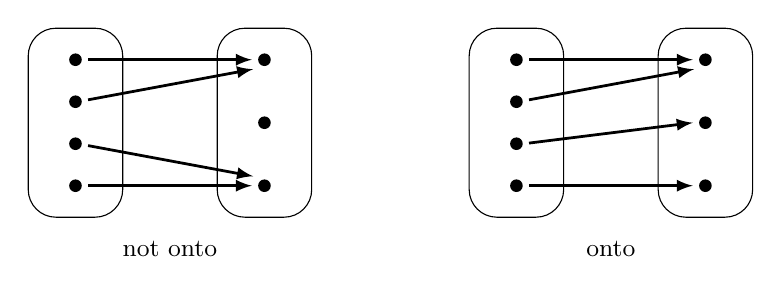
\begin{tikzpicture}[scale=0.8]
\begin{scope}
\draw[rounded corners=10pt] (-0.25,0) rectangle (1.25,3);
\draw[rounded corners=10pt] (2.75,0) rectangle (4.25,3);
\foreach \x in {0, 1, 2}{
\fill (3.5, {0.5 + \x}) circle (0.1);
}
\foreach \x in {0, 1, 2, 3}{
\fill (0.5, {0.5 + (2/3)*\x}) circle (0.1);
}
\draw[line width = 1, ->, >=latex] (0.7, 2.5) -- (3.3, 2.5); 
\draw[line width = 1, ->, >=latex] (0.7, 4/3 + 0.53) -- (3.32, 2.35); 
\draw[line width = 1, ->, >=latex] (0.7, 2/3 + 0.47) -- (3.32, 0.65); 
\draw[line width = 1, ->, >=latex] (0.7, 0.5) -- (3.3, 0.5); 
\node at (2, -0.5) {\small not onto};
\end{scope}


\begin{scope}[xshift = 70mm]
\draw[rounded corners=10pt] (-0.25,0) rectangle (1.25,3);
\draw[rounded corners=10pt] (2.75,0) rectangle (4.25,3);
\foreach \x in {0, 1, 2}{
\fill (3.5, {0.5 + \x}) circle (0.1);
}
\foreach \x in {0, 1, 2, 3}{
\fill (0.5, {0.5 + (2/3)*\x}) circle (0.1);
}
\draw[line width = 1, ->, >=latex] (0.7, 2.5) -- (3.3, 2.5); 
\draw[line width = 1, ->, >=latex] (0.7, 4/3 + 0.53) -- (3.32, 2.35); 
\draw[line width = 1, ->, >=latex] (0.7, 2/3 + 0.51) -- (3.3, 1.5); 
\draw[line width = 1, ->, >=latex] (0.7, 0.5) -- (3.3, 0.5); 
\node at (2, -0.5) {\small onto};
\end{scope}


\end{tikzpicture}
\end{equation*}



\textbullet\ \emph{one-to-one} if for any $\vv_{1}, \vv_{2}$ such that $\vv_{1}\neq \vv_{2}$ 
we have $F(\vv_{2}) \neq F(\vv_{2})$.

\begin{equation*}
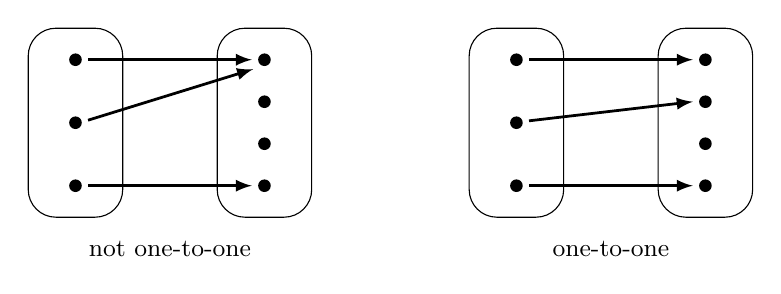
\begin{tikzpicture}[scale =0.8]
\begin{scope}
\draw[, rounded corners=10pt] (-0.25,0) rectangle (1.25,3);
\draw[, rounded corners=10pt] (2.75,0) rectangle (4.25,3);
\foreach \x in {0, 1, 2}{
\fill (0.5, {0.5 + \x}) circle (0.1);
}
\foreach \x in {0, 1, 2, 3}{
\fill (3.5, {0.5 + (2/3)*\x}) circle (0.1);
}
\draw[line width = 1, ->, >=latex] (0.7, 2.5) -- (3.3, 2.5); 
\draw[line width = 1, ->, >=latex] (0.7, 1.54) -- (3.32, 2.35); 
\draw[line width = 1, ->, >=latex] (0.7, 0.5) -- (3.3, 0.5); 
\node at (2, -0.5) {\small not  one-to-one};
\end{scope}

\begin{scope}[xshift = 70mm]
\draw[, rounded corners=10pt] (-0.25,0) rectangle (1.25,3);
\draw[, rounded corners=10pt] (2.75,0) rectangle (4.25,3);
\foreach \x in {0, 1, 2}{
\fill (0.5, {0.5 + \x}) circle (0.1);
}
\foreach \x in {0, 1, 2, 3}{
\fill (3.5, {0.5 + (2/3)*\x}) circle (0.1);
}
\draw[line width = 1, ->, >=latex] (0.7, 2.5) -- (3.3, 2.5); 
\draw[line width = 1, ->, >=latex] (0.7, 1.53) -- (3.3, 0.5 + 4/3); 
\draw[line width = 1, ->, >=latex] (0.7, 0.5) -- (3.3, 0.5); 

\node at (2, -0.5) {\small one-to-one};
\end{scope}
\end{tikzpicture}
\end{equation*}



\vskip 15mm


\begin{cbox}[Proposition]
Let $A$ be an $m\times n$ matrix. The following conditions are equivalent:

\benu
\item[\bf{1)}]  The matrix transformation $T_{A}\colon \R^{n} \to \R^{m}$ is onto. \\[-4mm]
\item[\bf{2)}]  $\Col(A) = \R^{m}$. \\[-4mm]
\item[\bf{3)}]  The matrix $A$ has a pivot position in every row. 
\eenu
\end{cbox}

\vfill

\begin{cbox}[Proposition]
Let $A$ be an $m\times n$ matrix. The following conditions are equivalent:

\benu
\item[1)]  The matrix transformation $T_{A}\colon \R^{n} \to \R^{m}$ is one-to-one. \\[-4mm]
\item[2)]  $\Nul(A) = \{0\}$.\\[-4mm]
\item[3)]  The matrix $A$ has a pivot position in every column. 
\eenu
\end{cbox}

\newpage


{\bf Example.} For the following $2\times 2$ matrix  $A$ check if the matrix transformation 
$T_{A}\colon \R^{2} \to \R^{2}$ is onto and if it is one-to-one. 
$$
A = 
\bbm
1 &  -1 \\
1 &   0 \\
 \ebm
$$

\vskip 70mm

{\bf Example.} For the following $3\times 4$ matrix  $A$ check if the matrix transformation 
$T_{A}\colon \R^{4} \to \R^{3}$ is onto and if it is one-to-one. 
$$
A = 
\bbm
 1 &  1 &  0 &  2  \\
-2 & -2 &  1 & -5  \\
 1 &  1 & -1 &  4  \\
 \ebm
$$






\newpage


\begin{cbox}[Proposition]
Let $A$ be an $m\times n$ matrix. If the matrix transformation $T_{A}\colon \R^{n} \to \R^{m}$
is both onto and one-to-one then we must have $m=n$ (i.e. $A$ must be a square matrix). 
\end{cbox}



\newpage



%---------------------------
%  Part 
%---------------------------
\lecture{Linear transformations and standard matrices}



{\bf Problem:} How to recognize if a function $f\colon \R^{n} \to \R^{m}$ is a matrix transformation? 


\vskip 10mm

{\bf Example.} Rotation by an angle $\theta$:


\btikz
\draw[->, line width = 2pt, black!40] (-3.5,0) -- (3.5,0);
\draw[->, line width = 2pt,  black!40] (0,-0.7) -- (0,4);
\draw[line width = 1.5pt] (0,0) -- ({cos(30)},{sin(30)}) arc [start angle = 30, end angle = 110, radius = 1] -- cycle;
\draw[->, line width = 2pt, blue] (0, 0) -- ({3*cos(30)},{3*sin(30)}) node[anchor = north west, pos=0.5] {\small $\vv$};
\draw[->, line width = 2pt, red] (0, 0) -- ({3*cos(110)},{3*sin(110)}) node[anchor = north east, pos=0.5] {\small $R_{\theta}(\vv)$};
\fill[black!40] (0,0) circle (0.1);
\node at ({1.35*cos(70)},{1.35*sin(70)}) {\small $\theta$};
\node at (0, -1.5) {$R_{\theta}\colon \R^{2} \to \R^{2}$};
\etikz

\newpage

\begin{cbox}[Definition]
A function $T\colon \R^{n} \to \R^{m}$ is a \emph{linear transformation} if it satisfies the following conditions:
\benu
\item[{\bf 1)}] $T(\uu + \vv) = T(\uu) + T(\vv)$ for all $\uu, \vv \in \R^{n}$ \\[-4mm]
\item[{\bf 2)}] $T(c\vv) = cT(\vv)$ for any $\vv \in \R^{n}$ and any scalar $c$. 
\eenu
\end{cbox}

\vskip 40mm

\begin{cbox}[Proposition]
Every matrix transformation is a linear transformation.
\end{cbox}


\newpage


\begin{cbox}[Theorem]
Every linear transformation $T\colon \R^{n} \to \R^{m}$ is a matrix transformation:
$$T = T_{A}$$
for some matrix $A$.
\end{cbox}


\newpage


\begin{cbox}[Corollary]
If $T\colon \R^{n} \to \R^{m}$ is a linear transformation then 
$T = T_{A}$ where $A$ is the matrix given by 
$$A = \bbm T(\ee_{1}) & T(\ee_{2}) & {\dots} & T(\ee_{n})   \\ \ebm$$
This matrix is called the \emph{standard matrix} of $T$. 
\end{cbox}

\vskip 10mm

{\bf Example.} Let $T \colon \R^{2} \to \R^{3}$ be the function given by 
$$
T\left(
\bbm
x_{1} \\
x_{2} \\
\ebm
\right) 
= 
\bbm[c]
x_{1} + x_{2} \\
0 \\
2x_{1} \\
\ebm
$$
Check if $T$ is a linear transformation. If it is, find its standard matrix. 


\newpage

{\bf Example.} Let $S \colon \R^{2} \to \R^{3}$ be the function given by 
$$
S\left(
\bbm
x_{1} \\
x_{2} \\
\ebm
\right) 
= 
\bbm[c]
1 + x_{2} \\
x_{2} \\
3x_{1} \\
\ebm
$$
Check if $S$ is a linear transformation. If it is, find its standard matrix. 



\newpage

\underline{\bf Back to rotations:}

\btikz
\draw[->, line width = 2pt, black!40] (-3.5,0) -- (3.5,0);
\draw[->, line width = 2pt,  black!40] (0,-0.7) -- (0,4);
\draw[line width = 1.5pt] (0,0) -- ({cos(30)},{sin(30)}) arc [start angle = 30, end angle = 110, radius = 1] -- cycle;
\draw[->, line width = 2pt, blue] (0, 0) -- ({3*cos(30)},{3*sin(30)}) node[anchor = north west, pos=0.5] {\small $\vv$};
\draw[->, line width = 2pt, red] (0, 0) -- ({3*cos(110)},{3*sin(110)}) node[anchor = north east, pos=0.5] {\small $R_{\theta}(\vv)$};
\fill[black!40] (0,0) circle (0.1);
\node at ({1.35*cos(70)},{1.35*sin(70)}) {\small $\theta$};
\node at (0, -1.5) {$R_{\theta}\colon \R^{2} \to \R^{2}$};
\etikz


\vfill

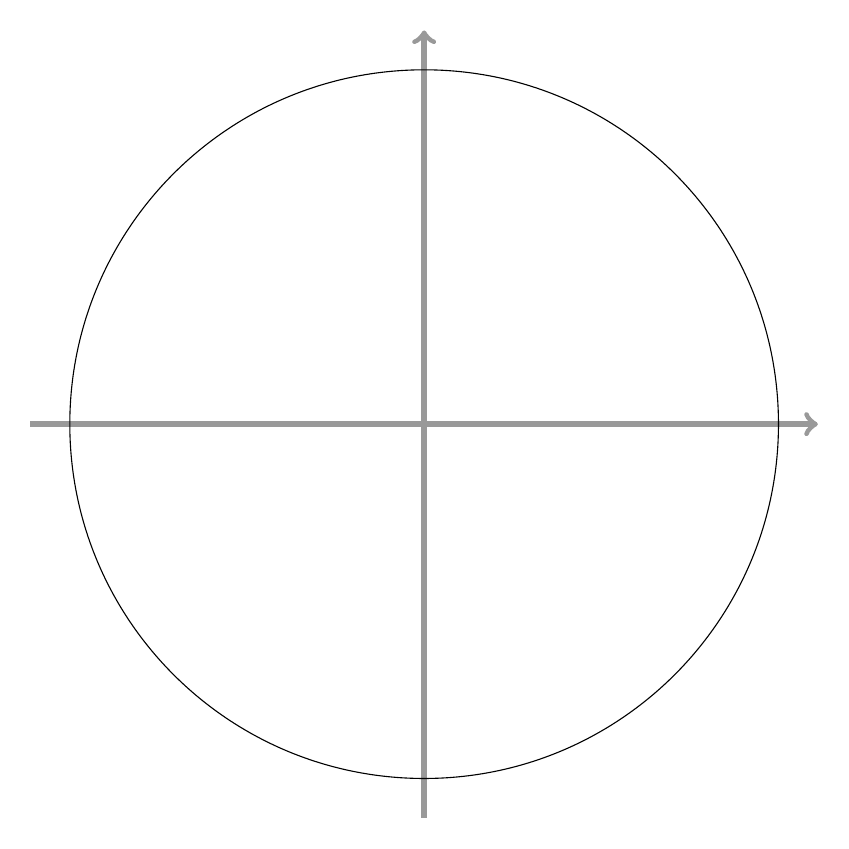
\begin{tikzpicture}
\draw[->, line width = 2pt, black!40] (-5,0) -- (5,0);
\draw[->, line width = 2pt,  black!40] (0,-5) -- (0,5);
\draw (0,0) circle (4.5);
\end{tikzpicture}


\newpage


\begin{cbox}[Proposition]
Let  $\ee_{1}, \ee_{2}, \dots, \ee_{n}$ be the standard basis of of $\R^{n}$. For any vectors 
$\vv_{1}, \vv_{n}, \dots, \vv_{n}\in \R^{m}$ there exists one and only one linear transformation 
$$T\colon \R^{n} \to \R^{m}$$
such that 
$$T(\ee_{1}) = \vv_{1}\ \ T(\ee_{2}) = \vv_{2},\ \  \dots, \ \   T(\ee_{n}) = \vv_{n}$$
The standard matrix of this linear transformation is given by 
$$A = \bbm \vv_{1} & \vv_{2} & {\dots} & \vv_{n} \\ \ebm$$
\end{cbox}

\newpage


%---------------------------
%  Part 
%---------------------------
\lecture{Matrix multiplication}


\textbf{\underline{Recall:}}

\vskip 5mm

\begin{enumerate}[leftmargin=*]
\item[\bf 1)] If $A$ is an $m\times n$ matrix then the function 
$$T_{A}\colon \R^{n} \to \R^{m}$$
defined by $T_{A}(\vv) = A\vv$ is called the matrix transformation associated to A. 

\vskip 20mm


\item[\bf 2)] A function $T\colon \R^{n} \to \R^{m}$ is a linear transformation if
\begin{enumerate}
\item[\bf (ii)] $T(\uu + \vv) = T(\uu) + T(\vv)$
\item[\bf (ii)] $T(c\vv) = cT(\vv)$
\end{enumerate}

\vskip 20mm

\item[\bf 3)] Every matrix transformation is a linear transformation. 

\vskip 20mm

\item[\bf 4)] Every linear transformation $T\colon \R^{n} \to \R^{m}$ is a matrix transformation:
$$T(\vv) = A\vv$$
where
$$A = \bbm T(\ee_{1}) &  T(\ee_{2}) &  {\dots} &  T(\ee_{n}) \\ \ebm$$
The matrix $A$ is called the standard matrix of $T$. 


\end{enumerate}



\newpage

\begin{center}
\underline{\bf Composition of linear transformations}
\end{center}


\vskip 30mm

\btikz
\begin{scope}[scale = 0.75]
\draw[->, line width = 2pt, black!40] (-3,0) -- (3,0);
\draw[->, line width = 2pt, black!40] (0,-3) -- (0,3);
\end{scope}
\begin{scope}[xshift = 65mm, scale = 0.75]
\draw[->, line width = 2pt, black!40] (-3,0) -- (3,0);
\draw[->, line width = 2pt, black!40] (0,-3) -- (0,3);
\end{scope}
\begin{scope}[xshift = 130mm, scale = 0.75]
\draw[->, line width = 2pt, black!40] (-3,0) -- (3,0);
\draw[->, line width = 2pt, black!40] (0,-3) -- (0,3);
\end{scope}
\etikz


\newpage


\begin{cbox}[Theorem]
If $S\colon \R^{n} \to \R^{m}$ and $T\colon \R^{m} \to \R^{k}$ are linear transformation then the composition 
$$T\circ S \colon \R^{n}\to \R^{k}$$
is also a linear transformation. 
\end{cbox}



\vfill

\begin{cbox}
{\bf Upshot.} The function $T\circ S$ is represented by some matrix $C$:
$$T\circ S(\vv) = C\vv$$
\end{cbox}

\newpage

{\bf Question.} Let  $S\colon \R^{n} \to \R^{m}$ and $T\colon \R^{m} \to \R^{k}$ be linear transformations, and let 
\bitem
\item $B$ is the standard matrix of $S$ \\[-4mm]
\item $A$ is the standard matrix of $T$
\eitem
What if the standard matrix of $T\circ S\colon \R^{n} \to \R^{k}$? 


\newpage

\begin{cbox}[Definition]
Let 
\begin{itemize}
\item $A$ be an $k\times m$ matrix
\item $B = \begin{bmatrix} \vv_{1} & \vv_{2} & {\dots}  & \vv_{n} \end{bmatrix}$ be an $m\times n$ matrix 
\end{itemize}
Then $A\cdot B$ is an $k\times n$ matrix given by  
$$A\cdot B = \begin{bmatrix} A\vv_{1} & A\vv_{2} & {\dots}  & A\vv_{n} \end{bmatrix}$$
\end{cbox}


\vfill

\textbf{Note.} The product $A\cdot B$ is defined only if 
$$(\text{number of columns of $A$})\  = \ (\text{number of rows of $B$})$$ 

\begin{equation*}
\begin{tikzpicture}
\draw[red!30, line width = 14] (-2.3, -0.58) -- (2.3, -0.58);
\draw[red!30, line width = 14, ->, >={Triangle[length = 10pt, width = 20pt]}] (-3.0, -0.9)   
..controls +(0.0, -1.5) and +(-1.5, 0.0)..  (-0.7, -3.05);
\draw[red!30, line width = 12, ->, >={Triangle[length = 10pt, width = 20pt]}] (3.0, -0.9)   
..controls +(0.0, -1.5) and +(1.5, 0.0)..  (0.7, -3.05);
\node at (-2.5,0) {$A$};
\node[anchor = base] at (-2.5,-0.7) {$k \times m$};
\node at (2.5,0) {$B$};
\node[anchor = base] at (2.5,-0.7) {$m \times n$};
\node at (0,-3.6) {$A\cdot B$};
\node at (0,-3.0) {$k \times n$};
\end{tikzpicture}
\end{equation*}


\newpage

{\bf Example.} 
\vskip 5mm 
$$
A = 
\bbm
0 & 1 & 2 \\
3 & 4 & 5 \\
\ebm
\ \ \ \ \ \ \ \ 
B  = 
\bbm
0 & -1 & 2 & 1 \\
4 &  5 & 1 & 0 \\
1 &  2 & 3 & 1 \\
\ebm
$$




\newpage


%---------------------------
%  Part 
%---------------------------
\lecture{Another view of matrix multiplication}


\vskip 10mm

$$
A = 
\bbm
a_{11} & {\dots} & a_{1m} \\
\vdots  &            &  \vdots \\
a_{k1} & {\dots} & a_{km} \\
\ebm
\ \ \ \ \ \ \ \ 
B = 
\bbm
b_{11} & {\dots} & b_{1n} \\
\vdots  &            &  \vdots \\
b_{m1} & {\dots} & b_{mn} \\
\ebm
$$
\vskip 10mm

$$
AB = 
\bbm
c_{11} & {\dots} & c_{1m} \\
\vdots  &            &  \vdots \\
c_{k1} & {\dots} & c_{km} \\
\ebm
$$


\vskip 20mm

$$
c_{ij} = 
\bbm
a_{i1} & a_{i2} & \dots & a_{im} \\
\ebm
\cdot 
\bbm
b_{1j} \\
b_{1j} \\
\vdots \\
b_{1j} \\
\ebm
= a_{i1}b_{1j} + a_{i2}b_{2j} + {\dots} + a_{im}b_{mj}
$$


\newpage

{\bf Example.} 
\vskip 5mm 
$$
A = 
\bbm
0 & 1 & 2 \\
3 & 4 & 5 \\
\ebm
\ \ \ \ \ \ \ \ 
B  = 
\bbm
0 & -1 & 2 & 1 \\
4 &  5 & 1 & 0 \\
1 &  2 & 3 & 1 \\
\ebm
$$



\newpage


\textbf{Example.} 
\begin{itemize}[leftmargin=*]
\item Acme Inc. makes two types of widgets: {\bf WG1} and {\bf WG2}. \\[-3mm]
\item Each widget must go though two processes: {\bf assembly} and {\bf testing}. \\[-3mm]
\item The number of hours required to complete each process is as follows:

\vskip 10mm

\begin{center}
\begin{tabular}{r | c  c}
          &\ \  {\bf \color{red} assembly } & {\bf \color{red} testing} \\[1mm]
 \hline
 & & \\[-3mm]
{\bf \color{red} WG1} &         3       &     1     \\[1mm]
{\bf \color{red} WG2} &         7       &     3      \\
\end{tabular}
\end{center}

\vskip 3mm

\item Acme Inc. has three plans in New York, Texas, and Minnesota. \\[-3mm]

\item Hourly cost (in dollars) of each process  in each plant  is as follows:

\vskip 10mm

\begin{center}
\hskip -18mm
\begin{tabular}{r | c  c  c}
          &\ \  {\bf \color{red} NY } & {\bf \color{red} TX}  & {\bf \color{red} MN} \\[1mm]
 \hline
 & & \\[-3mm]
{\bf \color{red} assembly} &     10      &     15    &   12     \\[1mm]
{\bf \color{red} testing}     &      15      &     20    &   15     \\
\end{tabular}
\end{center}

\end{itemize}

\vskip 5mm

{\bf\underline{Problem.}} What is the cost of producing each type of widgets in each plant?


\newpage


%---------------------------
%  Part 
%---------------------------
\lecture{Matrix algebra}


\begin{center}
\underline{\bf Other operations on matrices}
\end{center}

\vskip 10mm

{\bf 1) Addition.} 

\vskip 5mm

If 
$
A = 
\bbm[c]
a_{11} & {\dots} & a_{1n} \\
\vdots  &            &  \vdots \\
a_{m1} & {\dots} & a_{mn} \\
\ebm
$, 
$
B = 
\bbm[c]
b_{11} & {\dots} & b_{1n} \\
\vdots  &            &  \vdots \\
b_{m1} & {\dots} & b_{mn} \\
\ebm
$ 
 are $m\times n$ matrices then 


\vskip 10mm

$$
A + B = 
\bbm[c]
a_{11} + b_{11} & {\dots} & a_{1n} + b_{1n} \\
\vdots  &            &  \vdots \\
a_{m1} + b_{m1} & {\dots} & a_{mn} + b_{mn} \\
\ebm
 $$



\vfill 

{\bf Note.} The sum $A+B$ is defined only if $A$ and $B$ have the same dimensions. 

\newpage

{\bf 2) Scalar multiplication.} 

\vskip 5mm

If 
$
A = 
\bbm[c]
a_{11} & {\dots} & a_{1n} \\
\vdots  &            &  \vdots \\
a_{m1} & {\dots} & a_{mn} \\
\ebm
$, 
and $c$ is a scalar then 


\vskip 10mm

$$
cA = 
\bbm[c]
ca_{11}  & {\dots} & ca_{1n} \\
\vdots  &            &  \vdots \\
ca_{m1}  & {\dots} & ca_{mn} \\
\ebm
 $$

\newpage


\begin{center}
\underline{\bf Properties of matrix algebra}
\end{center}

\benu
\item[{\bf 1)}] $(AB)C = A(BC)$ \\
\item[{\bf 2)}] $(A+B)C = AC + BC$ \\
 $A(B+C) = AB + AC$\\
 
 \item[{\bf 3)}]  $I_{n} = $ the $n \times n$ identity matrix:
 $$
 I_{n} = 
 \bbm
 1 & 0 & {\dots} & 0 \\
  0 & 1 & {\dots} & 0 \\
  \vdots & \vdots & \ddots & \vdots \\
  0 & 0 & {\dots} & 1 \\
 \ebm
 $$
 
 If $A$ is an $m\times n$ matrix then 
 $$A\cdot I_{n} = A$$
  $$I_{m} \cdot A = A$$
\eenu


\newpage


\begin{center}
\underline{\bf Non-commutativity of matrix multiplication}
\end{center}

\vskip 5mm

{\bf 1)} If $AB$ is defined then $BA$ need not be defined.


\vskip 40mm


{\bf 2)} Even if both $AB$ and  $BA$ are both defined then usually 
$$AB\neq BA$$


\newpage


\begin{center}
\underline{\bf One more operation on matrices: matrix transpose}
\end{center}

\vskip 10mm

\begin{cbox}[Definition]
The transpose of a matrix $A$ is the matrix $A^{T}$ such that 
$$(\text{rows of $A^{T}$}) = (\text{columns of $A$})$$
\end{cbox}

\vfill

\underline{\bf Properties of transpose}
\vskip 5mm
\benu
\item[{\bf 1)}] $(A^{T})^{T} = A$ \\[-4mm]
\item[{\bf 2)}] $(A+B)^{T} = (A^{T} + B^{T}) $ \\[-4mm]
\item[{\bf 3)}] $(AB)^{T} = B^{T}A^{T}$
\eenu

\newpage


%---------------------------
%  Part
%---------------------------
\lecture{Inverse of a matrix}

\underline{\bf Operations on matrices so far:}

\vskip 5mm

\begin{tabular}{ll}
\textbullet\  addition/subtraction & {\color{red} $A\pm B$} \\[2mm] 
\textbullet\ scalar multiplication & {\color{red} $c\cdot A$} \\[2mm] 
\textbullet\ matrix multiplication  & {\color{red} $A\cdot B$} \\[2mm] 
\textbullet\ matrix transpose & {\color{red} $A^{T}$} \\
\end{tabular}

\vskip 10mm

\underline{\bf Next:} How to divide matrices? 

\vfill

\begin{cbox}[Definition]
A matrix $A$ is \emph{invertible} if there exists a matrix $B$ such that 
$$A\cdot B = B \cdot A = I$$
(where $I= $ the identity matrix). In such case we say that $B$ is the \emph{inverse} of $A$
and we write $B = A^{-1}$. 
\end{cbox}


\newpage

{\bf Example.}

\vskip 5mm

$$
A = 
\bbm
1 & -1 \\
1 & 1  \\
\ebm 
\  \text {is invertible, }
\ \ \  
A^{-1} = 
\bbm
\frac{1}{2} & \phantom{-}\frac{1}{2}  \\[2mm]
-\frac{1}{2}  & \frac{1}{2}   \\
\ebm
$$




\newpage

\begin{center}
\underline{\bf Matrix inverses and  matrix equations}
\end{center}


\begin{cbox}[Proposition]
If $A$ is an  invertible matrix then for any vector $\bb$ the equation $A\xx = \bb$ has exactly 
one solution.
\end{cbox}


\vskip 70mm

{\bf Example.} Solve the following matrix equation:

\vskip 3mm

$$
\bbm
1 & -1 \\
1 & 1 \\
\ebm
\cdot
\bbm
x_{1} \\
x_{2} \\
\ebm
= 
\bbm
1 \\
2 \\
\ebm
$$





\newpage


\newpage

\begin{center}
\underline{\bf Matrix inverses and matrix transformations}
\end{center}


\vskip 50mm

\btikz
\begin{scope}
\draw[->, line width = 2pt] (-1,0) -- (5,0);
\draw[->, line width = 2pt] (0,-1) -- (0,5);
\end{scope}
\begin{scope}[xshift = 90mm]
\draw[->, line width = 2pt] (-1,0) -- (5,0);
\draw[->, line width = 2pt] (0,-1) -- (0,5);
\end{scope}
\etikz

\newpage

{\bf Example.}

\vskip 5mm

$
A = 
\bbm
1 & 1 \\
1 & 1  \\
\ebm
$


\vskip 5mm

\btikz
\begin{scope}
\draw[->, line width = 2pt] (-1,0) -- (5,0);
\draw[->, line width = 2pt] (0,-1) -- (0,5);
\end{scope}
\begin{scope}[xshift = 100mm]
\draw[->, line width = 2pt] (-1,0) -- (5,0);
\draw[->, line width = 2pt] (0,-1) -- (0,5);
\end{scope}
\etikz

\vskip 20mm

{\bf Example.}

\vskip 5mm

$
A = 
\bbm
1 & 2 \\
2 & 4  \\
\ebm
$


\vskip 5mm

\btikz
\begin{scope}
\draw[->, line width = 2pt] (-1,0) -- (5,0);
\draw[->, line width = 2pt] (0,-1) -- (0,5);
\end{scope}
\begin{scope}[xshift = 100mm]
\draw[->, line width = 2pt] (-1,0) -- (5,0);
\draw[->, line width = 2pt] (0,-1) -- (0,5);
\end{scope}
\etikz

\newpage

\begin{cbox}
{\bf Upshot.} If an $m\times n$ matrix $A$ is invertible then the matrix transformation 
$T_{A}\colon \R^{n} \to \R^{m}$ must be one-to-one and onto.
\end{cbox}

\vskip 5mm

{\bf Recall:}
If $A$ be is $m\times n$ matrix then the matrix transformation $T_{A}\colon \R^{n} \to \R^{m}$ is:
\benu[leftmargin=*]
\item[\textbullet] \underline{onto} if and only if  $A$ has a pivot position in every row \\[-4mm]
\item[\textbullet] \underline{one-to-one} if and only if $A$ has a pivot position in every column.
\eenu


\vfill

\begin{cbox}[Theorem]
If $A$ is not a square matrix then it is not invertible. 

\vskip 3mm

If $A$ is a square matrix  then the following conditions are equivalent: 

\vskip 2mm

\benu
\item[\bf{1)}] $A$ is an invertible matrix. \\[-4mm]
\item[\bf{2)}] The matrix $A$ has a pivot position in every row and column. \\[-4mm]
\item[\bf{3)}] The reduced row echelon form of $A$ is the identity matrix $I_{n}$.
\eenu
\end{cbox}



\newpage

\begin{cbox}[Proposition]
If $A$ is an  $n\times n$ invertible matrix  then 
$$A^{-1} = \bbm \ww_{1} & \ww_{2} & {\dots} & \ww_{n} \\ \ebm$$
where $\ww_{i}$ is the solution of $A\xx = \ee_{i}$. 
\end{cbox}

\vskip 60mm

{\bf Example.}

\vskip 3mm

$A  = 
\bbm
1 & -1 \\
-1 & 1 \\
\ebm
$


\newpage


\begin{center}
{\bf 
\begin{tabular}{c}
Simplification: \\
How to solve several matrix equations with the same  \\
coefficient matrix at the same time
\end{tabular}
}
\end{center}

\begin{sframe}

\ 

\vskip -2mm





\btikz
\node[anchor = base] at (0,0)
{\begin{minipage}{100mm}
\begin{center}
$A\xx = \bb_{1}, \  A\xx = \bb_{2}, \ {\dots}, \  A\xx = \bb_{n}$
\vskip 2mm
{\color{red} matrix of equations}
\end{center}
\end{minipage}
};

\node[single arrow, draw,  minimum height = 10mm, minimum width = 40mm, anchor = tail,
single arrow head extend= 1mm,  single arrow tip angle = 130, text height=2ex, text depth=1ex, 
 line width = 2pt, red, text = red,  shape border rotate = 270]  
at (0, -1.5) {\small\emph{\begin{tabular}{c} \phantom{matrix} \end{tabular}}}; 

\node[anchor = base] at (0,-5.5)
{\begin{minipage}{100mm}
\begin{center}
$\bbm[c|cccc] A &  \bb_{1} & \bb_{2}  &  {\dots} & \bb_{n} \ebm$
\vskip 2mm
{\color{red} augmented matrix}
\end{center}
\end{minipage}
};

\node[single arrow, draw,  minimum height = 25mm, minimum width = 40mm, anchor = tail,
single arrow head extend= 1mm,  single arrow tip angle = 130, text height=2ex, text depth=1ex, 
 line width = 2pt, red, text = red,  shape border rotate = 270]  
at (0, -7) {\small\emph{\begin{tabular}{c}  row \\ reduction \end{tabular}}}; 

\node[anchor = base] at (0,-11)
{\begin{minipage}{100mm}
\begin{center}
$\bbm[c|cccc] \phantom{A} &  \phantom{\bb_{1}} & \phantom{\bb_{2}}  &  \phantom{{\dots}} & \phantom{\bb_{n}} \ebm$
\vskip 2mm
{\color{red} reduced matrix}
\end{center}
\end{minipage}
};


\node[single arrow, draw,  minimum height = 25mm, minimum width = 40mm, anchor = tail,
single arrow head extend= 1mm,  single arrow tip angle = 130, text height=2ex, text depth=1ex, 
 line width = 2pt, red, text = red,  shape border rotate = 270]  
at (0, -12.5) {\small\emph{\begin{tabular}{c}  read off \\ solutions \end{tabular}}}; 

\node[anchor = base] at (0,-16.5)
{\begin{minipage}{100mm}
\begin{center}
{solutions}
\end{center}
\end{minipage}
};

\etikz

\vskip 2mm

\end{sframe}

\newpage


{\bf Example.} Solve the vector equations $A\xx = \ee_{1}$ and $A\xx  = \ee_{2}$ where

\vskip 3mm

$$A  = 
\bbm
1 & -1 \\
1 & 1 \\
\ebm
\ \ \ \ \ \ 
\ee_{1} = 
\bbm
1 \\
0 \\
\ebm
\ \ \ \ \ \ 
\ee_{2} = 
\bbm
0 \\
1 \\
\ebm
$$


\newpage

\begin{center}
{\bf Summary:} \\
{\bf How to invert a matrix} \\
\end{center}

\vskip 5mm

\begin{sframe}

\vskip 5mm

{\bf Example:} 
$A = 
\bbm
1 & 1 \\
1 & 2 \\
\ebm
$

\vskip 5mm

{\bf 1)} Augment $A$ by the identity matrix.


\vskip 40mm

{\bf 2)}  Reduce the augmented matrix.


\vskip 40mm

{\bf 2)}  If after the row reduction the matrix on the left is the identity matrix, then $A$ is invertible and 
$$A^{-1} = \text{the matrix on the right}$$
Otherwise $A$ is not invertible. 

\vskip 40mm

\ 
\end{sframe}

\newpage

\underline{\bf Properties of matrix inverses}

\vskip 5mm

{\bf 1)} If $A$ is invertible then $A^{-1}$ is invertible and 
$$(A^{-1})^{-1} = A$$

\vskip 40mm

{\bf 2)} If $A, B$ are invertible then $AB$ is invertible and 
$$(AB)^{-1} = B^{-1}A^{-1}$$


\vskip 60mm

{\bf 3)} If $A$ is invertible then $A^{T}$ is invertible and 
$$(A^{T})^{-1} = (A^{-1})^{T}$$




\newpage

%---------------------------
%  Part
%---------------------------
\lecture{Application: Hill ciphers}

\underline{\bf Ciphers.}

\vskip 5mm

Cipher is an  algorithm for encrypting and decrypting data to conceal its meaning. 

\vskip 20mm
\begin{center}
\underline{\bf Basic working scheme of ciphers}
\end{center}

\vskip -5mm

\btikz[scale = 1.1, 
          line1/.style ={line width = 2pt, red, text=black},
          line2/.style  ={red!30, line width = 16},
          line3/.style  = {red!30, line width = 16, ->, >={Triangle[length = 14pt, width = 24pt]}}
          ]



\draw[line1] (0,0) rectangle +(3,1.5) node[pos=0.5] {\small \begin{tabular}{c} 
message \\ \end{tabular}};

\draw[line1] (0,-5.5) rectangle +(3,1.5) node[pos=0.5] {\small \begin{tabular}{c} 
encoded \\ message\end{tabular}};

\draw[line1] (6,-5.5) rectangle +(3,1.5) node[pos=0.5] {\small \begin{tabular}{c} 
encoded \\ message\end{tabular}};

\draw[line1] (6,0) rectangle +(3,1.5) node[pos=0.5] {\small \begin{tabular}{c} 
decoded \\ message\end{tabular}};

\draw[line1] (-2.5,-1.75) rectangle +(3,1.5) node[pos=0.5] {\small \begin{tabular}{c} 
encryption \\ key\end{tabular}};

\draw[line1] (8.5,-3.75) rectangle +(3,1.5) node[pos=0.5] {\small \begin{tabular}{c} 
decryption \\ key\end{tabular}};

\draw[line3, shorten >= 1pt, shorten <= 1pt, black!20, text=black] (3, -4.75) -- (6 , -4.75) 
    node[pos = 0.45] {\small \emph{send}};
\draw[line3, shorten >= 1pt, shorten <= 1pt, text=red] (1.5, 0) -- (1.5 , -4) 
    node[pos=0.5, anchor = west] {\small \emph{encryption}};
\draw[line3, shorten >= 1pt, shorten <= 1pt, text=red]  (7.5 , -4) -- (7.5, 0)
    node[pos=0.5, anchor = east,] {\small \emph{decryption}};

\draw[line2, shorten >= 1pt, shorten <= 1pt] (0.5, -1) arc (90: 0:1);
\draw[line2, shorten >= 1pt, shorten <= 1pt] (8.5, -3) arc (-90: -180:1);



\etikz

\newpage

{\bf Substitution cipher:} Replace each letter of the alphabet by some other letter. 

\ 

{\bf Example.}

\vskip -6mm

\btikz[scale = 0.6]
\newcounter{acount}
\setcounter{acount}{ `A}
\foreach \x in {1,...,26}{
	\draw (\x, 0) rectangle node { \small \char\value{acount}\addtocounter{acount}{1}} ({\x+1}, 1); 
	}
\foreach \x/\letter in {1/T, 2/V, 3/W, 4/X, 5/Y, 6/S, 7/C, 8/N, 9/O, 10/U, 11/Z, 12/A, 13/B, 14/P, 15/I, 16/M, 17/J, 18/Q, 19/R, 20/K, 21/D, 22/E, 23/F, 24/G, 25/H, 26/L}{
	\draw (\x, -1) rectangle node {\small \letter} ({\x+1}, 0); 
	}
\draw[red, ->, line width=2] (0.5, 1) -- node[yshift = -10pt, sloped] {\footnotesize encrypt} (0.5, -1) ;
\draw[red, ->, line width=2] (27.5, -1) -- node[yshift = -12pt, sloped] {\footnotesize decrypt} (27.5, 1) ;
\node[] at (13.5, -2.5) {encryption/decryption key};
\etikz

\ 

message: TOP SECRET

\newpage

{\bf Hill cipher:} Use matrix multiplication

\vskip 5mm

{\bf Example.}

\vskip -5mm

\btikz
\node at (0,0) {
$
A = 
\bbm
0 & 1 & 1 \\
1 & 1 & 0 \\
0 & 2 & 1 \\
\ebm
$
};
\node[red] at (0.47, -1.7) {\small
\begin{tabular}{c}
encryption key \\
invertible matrix \\
\end{tabular}
};
\begin{scope}[xshift = 60mm]
\node at (0,0) {
$
A^{-1} = 
\bbm
1 & 1 & -1 \\
-1 & 0 & 1 \\
2 & 0 & -1 \\
\ebm
$
};
\node[red] at (0.73, -1.7) {\small
\begin{tabular}{c}
decryption key \\
matrix inverse\\
\end{tabular}
};
\end{scope}
\etikz


message: TOP SECRET

\vskip 10mm

{\bf Encryption:}

\vskip 5mm

{\bf 1)} Replace letters by numbers:

\vskip -8mm

\ 
\btikz[scale = 0.65]
\setcounter{acount}{ `A}
\foreach \x in {1,...,26}{
	\draw (\x, 0) rectangle node { \small \char\value{acount}\addtocounter{acount}{1}} +(1, 1); 
	\draw (\x, -1) rectangle node { \small\x} +(1, 1); 
	}
\draw (0, 0) rectangle node { \small \underline{\phantom{A}}} +(1, 1); 
\draw (0, -1) rectangle node {\small 0} +(1, 1); 
\etikz

\vskip 10mm

\begin{minipage}{50mm}
{\bf 2)} Since the key is a $3\times 3$ matrix split the number sequence numbers in vectors with 3 entries each.
\end{minipage}


\vskip 10mm

\begin{minipage}{50mm}
{\bf 3)} Multiply each vector by the encryption matrix $A$.
\end{minipage}


\vfill

\begin{minipage}{50mm}
{\bf 4)} Write the new vectors as a sequence of numbers.
\end{minipage}


\newpage

{\bf We can do better,} but the next part will not work with an arbitrary invertible matrix $A$. It will work though e.g. if 
all entries of $A$ and $A^{-1}$ are integers. 

\ 

{\bf 5)} Reduce all numbers obtained in step 4 modulo 27. That is, add or subtract from each number a multiple 
of 27 to get a number between 0 and 26. 

\vskip 50mm

\begin{minipage}{50mm}
{\bf 6)}  Replace numbers by letters. 
\end{minipage}

\vskip 10mm 

{\bf Decryption.}


\vskip 5mm

\begin{minipage}{50mm}
{\bf 1)}  Replace letters by numbers, split into vectors, and multiply each vector by $A^{-1}$ 
\end{minipage}

\vskip 45mm

\begin{minipage}{50mm}
{\bf 2)}  Write the new vectors as a sequence of numbers, reduce each number modulo 27.   
\end{minipage}


\vfill

\begin{minipage}{50mm}
{\bf 3)}  Replace numbers by letters
\end{minipage}



\newpage



%---------------------------
%  Part
%---------------------------
\lecture{Application: Error correcting codes}

%% QR CODE
\begin{equation*}
\hskip 25mm
\begin{tikzpicture}[line3/.style  = {black!20, line width = 16, ->, >={Triangle[length = 14pt, width = 24pt]}}]
\node[fill=white, anchor= north west] at (0,0)
{\qrcode[height=35mm, level=H]{MTH 309  LINEAR ALGEBRA}};
\node[fill=white, anchor= north west] at (8,0)
{\qrcode[height=35mm, level=H]{MTH 309  LINEAR ALGEBRA}};
\fill[red!60!black] (10.3, -1.7) circle (0.8);


\fill[red!20] (10.3, -4.75) rectangle + (0.42, 0.5);
\draw[red, ->, line width =2] (10.51, -6.5) -- (10.51, -4.75) 
node[anchor = west, pos = 0.22, xshift = -5pt] {\small \emph{\begin{tabular}{l}transmission \\ error \end{tabular}}};
\node at (2, -4.5) {\tt {0\ 1\ 0\ 0\ 1}};
\node at (10, -4.5) {\tt{0\ 1\ 0\ 1\ 1}};
\draw[line3, shorten >= 15pt, shorten <= 15pt, black!20, text=black] (3.3, -4.5) -- (8.7 , -4.5) ;
%node[pos = 0.45] {\small \emph{send}};

\end{tikzpicture}
\end{equation*}
%% END QR CODE


\vskip 35mm


\begin{center}
\underline{\bf Basic  scheme of error correction}
\end{center}

\vskip -5mm

\btikz[scale = 1.1, 
          line1/.style ={line width = 2pt, red, text=black},
          line2/.style  ={red!30, line width = 16},
          line3/.style  = {red!30, line width = 16, ->, >={Triangle[length = 14pt, width = 24pt]}}
          ]



\draw[line1] (0,-2) rectangle +(3,1.5) node[pos=0.5] {\small \begin{tabular}{c} 
message \\ \end{tabular}};

\draw[line1] (0,-5.5) rectangle +(3,1.5) node[pos=0.5] {\small \begin{tabular}{c} 
encoded \\ message\end{tabular}};

\draw[line1] (6,-5.5) rectangle +(3,1.5) node[pos=0.5] {\small \begin{tabular}{c} 
received \\ message\end{tabular}};

\draw[line1] (6,-2) rectangle +(3,1.5) node[pos=0.5] {\small \begin{tabular}{c} 
decoded \\ message\end{tabular}};

\draw[line3, shorten >= 1pt, shorten <= 1pt, black!20, text=black] (3, -4.75) -- (6 , -4.75) 
    node[pos = 0.45, yshift = 1] {\small \emph{transmit}};
\draw[line3, shorten >= 1pt, shorten <= 1pt, text=red] (1.5, -2) -- (1.5 , -4) 
    node[pos=0.5, anchor = west] {\small \emph{encoding}};
\draw[line3, shorten >= 1pt, shorten <= 1pt, text=red]  (7.5 , -4) -- (7.5, -2)
    node[pos=0.5, anchor = east,] {\small \emph{decoding}};
\etikz

\vskip 10mm

{\bf Working assumption for this lecture:} We expect at most one transmission  error in any message up to 
20 bits long. 

\newpage

{\bf A simple error correcting code:} triple repeat.

\ 

message: 1011

\vfill


{\bf Problem:} The encoded message is 3 times longer than the original message.


\newpage

{\bf Better error correction:} Hamming (7,4) code.


\btikz
\node at (0,0) {
$
E = 
\bbm
1 & 0 & 0 & 0 \\
0 & 1 & 0 & 0 \\
0 & 0 & 1 & 0 \\
0 & 0 & 0 & 1 \\
0 & 1 & 1 & 1 \\
1 & 0 & 1 & 1 \\
1 & 1 & 0 & 1 \\
\ebm
$
};
\node[red] at (0.52, -2.8) {\small
\begin{tabular}{c}
encoding matrix \\
\end{tabular}
};
\begin{scope}[xshift = 70mm]
\node at (0,0) {
$
D = 
\bbm
0 & 1 & 1 & 1 & 1 & 0 & 0 \\
1 & 0 & 1 & 1 & 0 & 1 & 0 \\
1 & 1 & 0 & 1 & 0 & 0 & 1 \\
\ebm
$
};
\node[red] at (0.65, -1.4) {\small
\begin{tabular}{c}
decoding matrix \\
\end{tabular}
};
\end{scope}
\etikz

\ 

message: 10111101

\ 

{\bf Encoding.}

\vskip 3mm

{\bf 1)} Split the message into vectors with 4 entries, and multiply each vector by the encoding matrix $E$. 

\vskip 70mm

{\bf 2)} Reduce all numbers obtained in step 1 modulo 2. That is, add or subtract from each number a multiple 
of 2 to get either 0 or 1. 


\newpage
{\bf Encoded message:}

\vskip 10mm 
{\bf Received message:}


\vskip 10mm

{\bf Decoding.} Split the received  message into vectors with 7 entries, multiply each vector by the decoding matrix $D$,
and reduce modulo 2.  

\vfill 
{\bf Decoded message:}

\newpage
{\bf How the Hamming code works:}
\newpage


%---------------------------
%  Part
%---------------------------
\lecture{Determinants}

\underline{\bf Recall:} If an $n\times n$ matrix  $A$ is  invertible  then:  

\vskip 4mm

\benu
\item[\textbullet] the equation $A\xx=\bb$ has a unique solution for each $\bb\in \R^{n}$ \\[-4mm]
\item[\textbullet] the linear transformation $T_{A}\colon \R^{n} \to \R^{n}$, $T_{A}(\vv) = A\vv$ has an 
inverse function. 
\eenu


\vskip 10mm

Determinants recognize which matrices are invertible:


\begin{sframe}
\btikz[scale = 1.1, 
          line1/.style ={line width = 2pt, red, text=black},
          line2/.style  ={red!30, line width = 10},
          line3/.style  = {red!30, line width = 10, ->, >={Triangle[length = 12pt, width = 20pt]}}
          ]

\node[anchor = east] at (0,0) {$A$} ;
\node[anchor = west] at (3,0) {$\det A$};
\node[red] at (-0.33, -0.55) {\small matrix}; 
\node[red] at (3.7, -0.55) {\small number}; 

\draw[line3, shorten >= 5pt, shorten <= 5pt] (0, 0) -- (3 , 0);

\draw[line3, shorten >= 0pt, shorten <= 3pt, text=black] (4.5, 0.18) -- (5.5, 0.18) 
.. controls +(1, 0) and +(-1, 0).. (7.5, 1) -- (8.5 , 1)
node[anchor = west] {$= 0$ if $A$ is not invertible};
\draw[line3, shorten >= 0pt, shorten <= 3pt, text=black] (4.5, -0.18) -- (5.5, -0.18) 
.. controls +(1, 0) and +(-1, 0).. (7.5, -1) -- (8.5 , -1)
node[anchor = west]  {$\neq 0$ if $A$ is invertible};
\etikz
\end{sframe}

\vskip 10mm

{\bf Example:} Determinant for a $1\times 1$ matrix. 
$$A = \bbm a \ebm$$

\newpage 


{\bf Example:} Determinant for a $2\times 2$ matrix. 
$$A = \bbm a & b \\ c & d \\ \ebm$$


\newpage

\begin{cbox}[Definition]
If $A$ is an  $n\times n$  matrix  then for $1\leq i, j \leq n$ the 
\emph{$(i, j)$-minor} of $A$ is the matrix $A_{ij}$ obtained by deleting 
the $i^{\text{th}}$ row and $j^{\text{th}}$ column of $A$. 
\end{cbox}

\vskip 10mm 

{\bf Example.}

\vskip 5mm
$A = 
\bbm
1 & 2 & 3 \\
4 & 5 & 6 \\
7 & 8 & 9 \\
\ebm
$

\newpage


\begin{cbox}[Definition]
Let $A$ be an  $n\times n$  matrix
$$
A = 
\begin{bmatrix}
a_{11} &  {\dots} & a_{1n} \\
\vdots &  & \vdots \\
a_{n1} &  {\dots} & a_{nn} \\
\end{bmatrix}
$$

{\bf 1)} If $n=1$, i.e. $A = \bbm a_{11} \ebm$,  then $\det A = a_{11}$

\vskip 3mm

{\bf 2)} If $n>1$ then 
\begin{alignat*}{3}
\det A = 
&&(-1)^{1+1} a_{11}\cdot \det A_{11} \\
&+&(-1)^{1+2} a_{12}\cdot \det A_{12} \\
&\dots& \dots \ \ \ \dots \ \ \ \dots \\
&+&(-1)^{1+n} a_{1n}\cdot \det A_{1n} \\
\end{alignat*}
\end{cbox}

\vskip 5mm

{\bf Example.} ($n=2$)

\vskip 3mm

$A = 
\bbm
1 & 2 \\
3 & 4 \\
\ebm
$

\vfill

\begin{cbox}[Note]
If $A$ is a $2\times 2$ matrix
$$A = 
\bbm
a_{11} & a_{12} \\
a_{21} & a_{22} \\
\ebm
$$
then $\det A = a_{11}\cdot a_{22} - a_{12}\cdot a_{21}$
\end{cbox}

\newpage

{\bf Example.} (n=3)

\vskip 3mm

$A = 
\bbm
1 & 2 & 3 \\
4 & 5 & 6 \\
7 & 8 & 9 \\
\ebm
$

\newpage

\begin{center}
\underline{\bf{ A direct way of computing the determinant of a $\mathbf{3\times 3}$ matrix}}
\end{center}


\vskip 15mm

$$A = 
\bbm
1 & 2 & 3 \\
4 & 5 & 6 \\
7 & 8 & 9 \\
\ebm
$$


\newpage

{\bf Example} (n=4)

\vskip 3mm

$A = 
\bbm
1 & 0 & 2 & 0 \\
0 & 4 & 0 & 1 \\
2 & 1 & 6 & 1 \\
3 & 5 & 7 & 0 \\
\ebm
$

\newpage

{\bf Note.} In order to compute the determinant of an $n\times n$ matrix in this way we need to compute: 

\begin{flushright}
\begin{tabular}{rl}
$n$ & determinants of $(n-1)\times (n-1)$ matrices \\
$n(n-1)$ & determinants of $(n-2)\times (n-2)$ matrices \\
$n(n-1)(n-2)$ & determinants of $(n-3)\times (n-3)$ matrices \\
$\dots \ \ \ \dots \ \ \ \dots \ \ \ \dots $ &  $ \ \ \ \dots \ \ \ \dots \ \ \ \dots \ \ \ \dots \ \ \ \dots \ \ \ \dots \ \ \ \dots$ \\
$n(n-1)(n-2)\cdot {\dots} \cdot 3$ & determinants of $2 \times 2$ matrices \\
\end{tabular}
\end{flushright}

\vskip 40mm

E.g. for a $25\times 25$ matrix we would need to compute
$$25\cdot 24 \cdot 23 \cdot{\dots}\cdot 3 =  7,755,605,021,665,492,992,000,000$$
determinants of $2\times 2$ matrices. 

\vskip 30mm

\underline{\bf Next:} How to compute determinants faster. 


%---------------------------
%  Part
%---------------------------
\lecture{Determinants and cofactor expansion}

\begin{cbox}[Definition]
If $A$ is an $n\times n$ matrix and $1\leq i, j \leq n$ then the \emph{$ij$-cofactor of $A$} is the number 
$$C_{ij} = (-1)^{i+j}\det A_{ij}$$
\end{cbox}

\vskip 5mm

{\bf Example.}
\vskip 3mm
$A = 
\bbm
1 & 2 & 3 \\
4 & 5 & 6 \\
7 & 8 & 9 \\
\ebm
$

\vfill

{\bf Note.} By the definition of the determinant we have:
$$\det A = a_{11}C_{11} + a_{12}C_{12} + {\dots} + a_{1n}C_{1n}$$

\newpage

\begin{cbox}[Theorem]
Let $A$ be an $n\times n$ matrix. 
\vskip 3mm
{\bf 1)} For any $1\leq i \leq n$ we have 
$$\det A = a_{i1}C_{i1} + a_{i2}C_{i2} + {\dots} + a_{in}C_{in}$$
(cofactor expansion across the $i^{{\text th}}$ row).
\vskip 3mm
{\bf 2)} For any $1\leq j \leq n$ we have 
$$\det A = a_{1j}C_{1j} + a_{2j}C_{2j} + {\dots} + a_{nj}C_{nj}$$
(cofactor expansion down the $j^{{\text th}}$ column).
\end{cbox}

\vskip 5mm

{\bf Example.}

\vskip 3mm

$
A = 
\bbm
1 & 3 & 0 & 4 \\
0 & 4 & 6 & 1 \\
2 & 1 & 0 & 3 \\
0 & 5 & 0 & 0 \\
\ebm
$

\newpage

{\bf Example.} Compute the determinant of the following matrix:


\vskip 10mm


{\small
$\left[{
\begin{tabular}{rrrrrrrrrrrrrrrrrrrrr}
1 & 0 & 0 & 3 & 0 & 0 & 2& 0 & 3 & 0 & 0 & 0 & 0 & $e$ & 0 & 0 & 0 & 3 & 0 & 0 & 0 \cr
0 & 2 & 0 & 0 & $\pi$ & 0 & 0 & 0 & 6 & 0 & 0 & 5 & 6 & 0 & 2 & 0 & 7 & 0 & 0 & 0 & 0 \cr
0 & 0 & 1 & 0 & 0 & 0 & 0 & 0 & 11 & 0 & 0 & 0 & 0 & 0 & 7 & 0 & 0 & 0 & 0 & 0 & 0 \cr
0 & 0 & 0 & $-\frac{1}{2}$ & 0 & 0 & 0& 0 & 4 & 0 & 0 & 2 & 0 & 4 & 0 & 2 & 0 & 0 & 0 & 0 & 0 \cr
0 & 0 & 0 & 0 & 0 & 0 & 0 & 0 & 0 & 0 & 0 & 0 & 0 & 0 & 0 & 0 & 0 & 1 & 0 & 0 & 0 \cr
0 & 0 & 0 & 0 & 0 & $-1$ &  0 & 0 & 0 & 0 & 9 & 0 & 0 & 0 & 2 & 1 & 2 & 3 & 4 & 0 & 0 \cr
0 & 0 & 0 & 0 & 0 & 0 & 3 & 1 & 0 & 0 & $-1$ & 0 & 0 & 0 & 0 & 0 & 5 & 0 & 0 & 0 & 0 \cr
0 & 0 & 0 & 0 & 0 & 0 & 2 & 1 & 0 & 0 & 0 & 0 & 0 & 0 & 12 & 0 & 0 & 0 & 0 & 0 & 0 \cr
0 & 0 & 0 & 0 & 0 & 0 & 0 & 0 & 2 & 0 & 0 & 0 & 0 & 0 & 0 & $-1$ & 0 & 0 & 4 & 0 & 0 \cr
0 & 0 & 0 & 0 & 0 & 0 & 0 & 0 & 0 & 3 & 0 & 0 & 2 & 7 & 0 & $-4$ & 0 & 0 & 3 & 0 & 0 \cr
0 & 0 & 0 & 0 & 0 & 0 & 0 & 0 & 0 & 0 & 1 & 0 & 0 & 0 & 0 & 3 & 0 & 0 & 2 & 0 & 0 \cr
0 & 0 & 0 & 0 & 0 & 0 & 0 & 0 & 0 & 0 & 0 & 2 & 0 & 0 & 0 & 0 & 0 & 0 & 0 & 6 & 0 \cr
0 & 0 & 0 & 0 & 0 & 0 & 0 & 0 & 0  & 0 & 0 & 0 & $\frac{1}{4}$ & 0 & 0 & 0 & 0 & 0 & 0 & 0 & 0 \cr
0 & 0 & 0 & 0 & 0 & 0 & 0 & 0 & 0 & 0 & 0 & 0 & 0 & $\frac{1}{5}$ & 0 & 1 & 0 & 4 & 3 & 2 & 1 \cr
0 & 0 & 0 & 0 & 0 & 0 & 0 & 0 & 0 & 0 & 0 & 0 & 0 & 0 & 1 & 0 & 0 & 0 & 0 & 0 & 0 \cr
0 & 0 & 0 & 0 & 0 & 0 & 0 & 0 & 0 & 0 & 0 & 0 & 0 & 0 & 0 & 1 & 0 & 0 & 8 & 7 & 7 \cr
0 & 0 & 0 & 0 & 0 & 0 & 0 & 0 & 0 & 0 & 0 & 0 & 0 & 0 & 0 & 0 & 2 & 0 & 0 & 0 & 0 \cr
0 & 0 & 0 & 0 & 0 & 0 & 0 & 0 & 0 & 0 & 0 & 0 & 0 & 0 & 0 & 0 & 0 & 1 & 0 & $-1$ & 0 \cr
0 & 0 & 0 & 0 & 0 & 0 & 0 & 0 & 0 & 0 & 0 & 0 & 0 & 0 & 0 & 0 & 0 & 0 & 0 & 0 & 1 \cr
0 & 0 & 0 & 0 & 0 & 0 & 0 & 0 & 0 & 0 & 0 & 0 & 0 & 0 & 0 & 0 & 0 & 1 & 1 & 1 & 0 \cr
0 & 0 & 0 & 0 & 2 & 8 & 9 & 0 & 3 & 3 & 2 & 5 & 6 & 3 & 8 & 9 & 2 & 6 & 2 & 2 & 1 \cr
\end{tabular}
}\right]$
}


\newpage

\begin{cbox}[Definition]
An square matrix is \emph{upper triangular} is all its entries below the main diagonal are 0. 
\end{cbox}

\vskip 10mm

$$
A = 
\begin{bmatrix}
a_{11}  & a_{12}  & a_{13} & \dots  & a_{1n} \\
0          & a_{22}  & a_{23} & \dots   & a_{2n} \\
0          &  0         & a_{33} & \dots   & a_{3n} \\
\vdots   &  \vdots & \vdots  & \ddots & \vdots \\
0           & 0         & 0          & \dots   & a_{nn} \\
\end{bmatrix}
$$

\vskip 10mm

\begin{cbox}[Proposition]
If $A$ is an upper triangular matrix as above then 
$$\det A = a_{11}\cdot a_{22}\cdot {\dots}\cdot a_{nn}$$ 
\end{cbox}


%---------------------------
%  Part
%---------------------------
\lecture{Determinants and row reduction}


\underline{\bf Recall:} If $A$ is an upper triangular matrix:

$$
A = 
\begin{bmatrix}
a_{11}  & a_{12}  & a_{13} & \dots  & a_{1n} \\
0          & a_{22}  & a_{23} & \dots   & a_{2n} \\
0          &  0         & a_{33} & \dots   & a_{3n} \\
\vdots   &  \vdots & \vdots  & \ddots & \vdots \\
0           & 0         & 0          & \dots   & a_{nn} \\
\end{bmatrix}
$$

then $\det A = a_{11}\cdot a_{22}\cdot {\dots}\cdot a_{nn}$.

\vskip 20mm

{\bf Note.} If $A$ is a square matrix then the  row echelon form of $A$ is always upper triangular. 


\newpage

\begin{cbox}[Theorem]
Let $A$ and $B$ be $n\times n$ matrices.

\vskip 3mm

\textbf{1)} If $B$ is obtained from $A$ by interchanging two rows (or two columns) then 
$$\det B = -\det A$$

\textbf{2)} If $B$ is obtained from $A$ by multiplying one row (or one column) of $A$ by 
a scalar $k$ then 
$$\det B = k\cdot \det A$$

\textbf{2)} If $B$ is obtained from $A$ by adding a multiple of one row of $A$ to another row
(or adding a multiple of one column to another column) then 
$$\det B = \det A$$
\end{cbox}

\vskip 5mm

{\bf Example.} 

\vskip 3mm

$A = 
\bbm
1 & 2 & 3 \\
1 & 0 & 7 \\
2 & 5 & 1 \\
\ebm
$

\newpage

\begin{center}
\underline{\bf Computation of determinants via row reduction}
\end{center}


\textbf{Idea.}
To compute $\det A$, row reduce $A$ to the row echelon form. Keep track how the determinant 
changes at each step of the row reduction process. 

\vskip 10mm

{\bf Example.} Compute $\det A$  where
$$A = 
\bbm
0 & 1 & 2 & 3 \\
2 & 4 & 0 & 10 \\
3 & 4 & 1 & 7 \\
-2 & 5 & 3 & 0  \\
\ebm
$$


\newpage


\begin{cbox}[Theorem]
If $A$ is a square matrix then $A$ is invertible if and only if $\det A \neq 0$
\end{cbox}

\vskip 5mm

\underline{\bf Recall:} $A$ is invertible if and only if its reduced row echelon form is the identity matrix. 

\newpage


\underline{\textbf{Further properties of determinants}}

\vskip 5mm

\benu
\item[\textbf{1)}]  $\det(A^{T}) = \det A$ \\[-4mm]
\item[\textbf{2)}]  $\det(AB)= (\det A)\cdot(\det B)$ \\[-4mm]
\item[\textbf{3)}]  $\det (A^{-1})= (\det A)^{-1}$
\eenu


\vskip 10mm


\textbf{Note.}  In general $\det(A+B)\neq \det A + \det B$.



%---------------------------
%  Part
%---------------------------
\lecture{Cramer's rule}

\underline{\bf Recall:} If $A$ is square matrix then the \emph{$ij$-cofactor of $A$} is the number 
$$C_{ij} = (-1)^{i+j}\det A_{ij}$$

\vskip 10mm

\begin{cbox}[Definition]
If $A$ is an $n\times n$ matrix then the \emph{adjoint} (or \emph{adjugate}) of $A$
is the matrix

$$\text{adj} A = 
\begin{bmatrix}
C_{11} & C_{12}  &  \cdots & C_{1n} \\
C_{21} & C_{22}  &  \cdots & C_{2n}\\
\vdots    & \vdots    &              & \vdots\\
C_{n1} & C_{n2}  &  \cdots & C_{nn}\\
\end{bmatrix}^{T}
=
\begin{bmatrix}
C_{11} & C_{21}  &  \cdots & C_{n1}\\
C_{12} & C_{22}  &  \cdots & C_{n2}\\
\vdots    & \vdots    &              & \vdots\\
C_{1n} & C_{2n}  &  \cdots & C_{nn}\\
\end{bmatrix}
$$
\end{cbox}

\begin{cbox}[Theorem]
If $A$ is an invertible matrix then 
$$A^{-1} = \frac{1}{\det A}\cdot \text{adj} A$$
\end{cbox}


\newpage

{\bf Example.} Compute $A^{-1}$ for 
$$A = 
\bbm
1 & 1 & 2 \\
4 & 0 & 0 \\
1 & 1 & 1 \\
\ebm
$$

\newpage

\underline{\bf Recall:} If $A$ is an invertible matrix then the equation $A\xx = \bb$ has only one solution: $\xx = A^{-1}\bb$.

\vskip 5mm

\begin{cbox}[Definition]
If $A$ is an $n\times n$ matrix and  $\bb\in \R^{n}$ then 
$A_{i}(\bb)$ is the matrix obtained by replacing the $i^{\text{th}}$ column of $A$ with $\bb$.
\end{cbox}

\vskip 5mm

{\bf Example.} 
$$A = 
\bbm
1 & 2 & 3 \\
4 & 5 & 6 \\
7 & 8 & 9 \\
\ebm 
\ \ \ \ \ \ 
\bb = 
\bbm
10 \\
20 \\
30 \\
\ebm
$$

\vskip 50mm

\begin{cbox}[Theorem (Cramer's Rule)]
If $A$ is an $n\times n$ invertible matrix and $\bb\in \R^{n}$ then the unique 
solution of the equation 
$$A\xx=\bb$$
is given by 
$$
\xx = \frac{1}{\det A}
\begin{bmatrix}
\det A_{1}(\bb)\\
\vdots\\
\det A_{n}(\bb)\\
\end{bmatrix}
$$
\end{cbox}


\newpage

{\bf Example.} Solve the equation
$$
\bbm
1 & 1 & 2 \\
4 & 0 & 0 \\
1 & 1 & 1 \\
\ebm
\cdot 
\bbm
x_{1} \\
x_{2} \\
x_{3} \\
\ebm
= 
\bbm
1 \\
2 \\
3 \\
\ebm
$$

%---------------------------
%  Part
%---------------------------
\lecture{Geometric interpretation of determinants}

\underline{\bf Recall:}

\begin{sframe}
\btikz[scale = 1.1, 
          line1/.style ={line width = 2pt, red, text=black},
          line2/.style  ={red!30, line width = 10},
          line3/.style  = {red!30, line width = 10, ->, >={Triangle[length = 12pt, width = 20pt]}}
          ]

\node[anchor = east] at (0,0) {$A$} ;
\node[anchor = west] at (3,0) {$\det A$};
\node[red] at (-0.33, -0.55) {\small matrix}; 
\node[red] at (3.7, -0.55) {\small number}; 

\draw[line3, shorten >= 5pt, shorten <= 5pt] (0, 0) -- (3 , 0);

\draw[line3, shorten >= 0pt, shorten <= 3pt, text=black] (4.5, 0.18) -- (5.5, 0.18) 
.. controls +(1, 0) and +(-1, 0).. (7.5, 1) -- (8.5 , 1)
node[anchor = west] {$= 0$ if $A$ is not invertible};
\draw[line3, shorten >= 0pt, shorten <= 3pt, text=black] (4.5, -0.18) -- (5.5, -0.18) 
.. controls +(1, 0) and +(-1, 0).. (7.5, -1) -- (8.5 , -1)
node[anchor = west]  {$\neq 0$ if $A$ is invertible};
\etikz
\end{sframe}


\vfill

{\bf Note.} Any two vectors in $\R^{2}$ define a parallelogram:


\vskip 5mm

\btikz[
          scale = 2.5,
          line1/.style ={line width = 3, ->}
          ]

\draw[fill=black!20] (0,0) -- ++(2,0) -- ++(1,1) -- ++(-2, 0) -- cycle;
\draw[red, line1] (0,0) -- (2, 0) node[pos=0.55, yshift = -3pt, anchor = north] {$\vv_{1}$};
\draw[blue, line1] (0,0) -- (1, 1) node[pos=0.5, anchor = south east] {$\vv_{2}$};
\fill[red] (0,0) circle (0.05);
\etikz

\vskip 10mm

\begin{cbox}[Notation]
$$\text{area}(\vv_{1}, \vv_{2}) = 
\begin{pmatrix}
\text{area of the parallelogram} \\
\text{defined by $\vv_{1}$ and $\vv_{2}$}
\end{pmatrix}
$$
\end{cbox}


\newpage

\begin{cbox}[Theorem]
If $\vv_{1}, \vv_{2}\in \R^{2}$ then 
$$\text{area}(\vv_{1}, \vv_{2}) = \left | \det \bbm \vv_{1} & \vv_{2} \\ \ebm \right | $$
\end{cbox}

\vskip 5mm

\emph{Idea of the proof.}

\vskip 3mm

$\vv_{1} = \bbm a \\ b \ebm$, \ \  $\vv_{2} = \bbm c \\ d \ebm$



\definecolor{MyGreen}{RGB}{230, 255, 153}
\definecolor{MyYellow}{RGB}{255, 230, 153}
\definecolor{MyPink}{RGB}{255, 204, 204}
\definecolor{MyBlue}{RGB}{179, 230, 255}



\btikz[
          scale = 2.5,
          line1/.style ={line width = 4, ->},
          line2/.style ={line width = 1.5, join=bevel}
          ]


\begin{scope}
\coordinate (A) at (0,0);
\coordinate (B) at (3,1);
\coordinate (C) at (1,2);
\coordinate (D) at (4,3);

\coordinate (E) at (4,0);
\coordinate (F) at (0,3);

\coordinate (BX) at (3,0);
\coordinate (BX') at (3,3);
\coordinate (BY) at (0,1);
\coordinate (BY') at (4,1);
\coordinate (CX) at (1,0);
\coordinate (CX') at (1,3);
\coordinate (CY) at (0,2);
\coordinate (CY') at (4,2);
\coordinate (DY) at (0,3);
\coordinate (DX) at (4,0);

\coordinate (OFFY) at (0.1,0);
\coordinate (OFFX) at (0, 0.1);


\draw[line width = 1, ->] ($(A) - (0, 0.4)$) -- ($(F) + (0, 0.6)$);
\draw[line width = 1, ->] ($(A) - (0.4, 0)$) -- ($(E) + (0.6, 0)$);

\draw[line width = 1] ($(CX)-(OFFX)$) -- ($(CX')+(OFFX)$) node[pos = -0.015, anchor=north] {\small c}  node[pos=1.015, anchor=south] {c};
\draw[line width = 1] ($(BX)-(OFFX)$) -- ($(BX')+(OFFX)$) node[pos = -0.015, anchor=north] {\small a}  node[pos=1.015, anchor=south] {a};
\draw[line width = 1] ($(DX)-(OFFX)$) -- ($(D)+(OFFX)$) node[pos = -0.015, anchor=north] {\small a+c}  node[pos=1.015, anchor=south] {a+c};


\draw[line width = 1] ($(CY)-(OFFY)$) -- ($(CY')+(OFFY)$) node[pos = -0.015, anchor=east] {\small d}  node[pos=1.015, anchor=west] {d};
\draw[line width = 1] ($(BY)-(OFFY)$) -- ($(BY')+(OFFY)$) node[pos = -0.015, anchor=east] {\small b}  node[pos=1.015, anchor=west] {b};
\draw[line width = 1] ($(DY)-(OFFY)$) -- ($(D)+(OFFY)$) node[pos = -0.015, anchor=east] {\small b+d}  node[pos=1.015, anchor=west] {b+d};

\draw[line2, fill = MyYellow] (A) -- (B) -- (BX) -- cycle; 
\draw[line2, fill = MyYellow] (C) -- (CX') -- (D) -- cycle;

\draw[line2, fill = MyGreen] (BX) -- (B) -- (BY') -- (E) -- cycle;
\draw[line2, fill = MyGreen] (CY) -- (C) -- (CX') -- (F) -- cycle;

\draw[line2, fill = MyBlue] (B) -- (BY') -- (D) -- cycle;
\draw[line2, fill = MyBlue] (A) -- (CY) -- (C) -- cycle;


\draw[line2, fill=MyPink, text=black] (A) -- (B) -- (D) -- (C) -- cycle;
\node at (2, 1.5) {$P$};
\draw[line width = 2pt] (A) -- (E) -- (D) -- (F) -- cycle;

\draw[red, line1] (A) -- (B) node[pos=0.55, yshift = -3pt, anchor = north] {$\vv_{1}$};
\draw[blue, line1] (A) -- (C) node[pos=0.5, anchor = south east] {$\vv_{2}$};
\fill[] (0,0) circle (0.05);
\end{scope}
\begin{scope}[xshift = 55mm]
\fill[MyPink, text=black] (0, 2.7) rectangle node[anchor=west, xshift = -27pt] {\small $\text{area}(P)$} (0.75, 3.0);

\fill[MyYellow, text=black] (0, 0.1+ 5*0.433) rectangle node[anchor=west, xshift = -27pt] {\small $\frac{1}{2}ab$} (0.75, 0.4+5*0.433);
\node at (-0.1, 0.25+5*0.433) {\small $+$};

\fill[MyYellow, text=black] (0, 0.1+ 4*0.433) rectangle node[anchor=west, xshift = -27pt] {\small $\frac{1}{2}ab$} (0.75, 0.4 +4*0.433);
\node at (-0.1, 0.25+4*0.433) {\small $+$};

\fill[MyBlue, text=black] (0, 0.1+ 3*0.433) rectangle node[anchor=west, xshift = -27pt] {\small $\frac{1}{2}cd$} (0.75, 0.4 +3*0.433);
\node at (-0.1, 0.25+3*0.433) {\small $+$};

\fill[MyBlue, text=black] (0, 0.1+ 2*0.433) rectangle node[anchor=west, xshift = -27pt] {\small $\frac{1}{2}cd$} (0.75, 0.4 +2*0.433);
\node at (-0.1, 0.25+2*0.433) {\small $+$};

\fill[MyGreen, text=black] (0, 0.1+ 0.433) rectangle node[anchor=west, xshift = -27pt] {\small $cb$} (0.75, 0.4 + 0.433);
\node at (-0.1, 0.25 + 0.433) {\small $+$};

\fill[MyGreen, text=black] (0, 0.1) rectangle node[anchor=west, xshift = -27pt] {\small $cb$} (0.75, 0.4);
\node at (-0.1, 0.25) {\small $+$};

\draw[line width = 1pt] (-0.5, 0.) -- (0.75, 0.);
\node[anchor = east, xshift=5pt] at (0.75, -0.2) {\small $(a+c)(b+d)$};
\end{scope}
\etikz


\newpage

{\bf Example.}
\vskip 5mm

\begin{tikzpicture}
\node at (0,0) {$\vv_{1} = \bbm 2 \\ 3 \ebm$,  \ \ $\vv_{2} = \bbm 2 \\ -2 \ebm$};
\begin{scope}[xshift = 80mm, yshift = -30mm]
\foreach \x in {-1,...,6}{
\draw[help lines] (\x, -3) -- (\x, 4);
}
\foreach \y in {-3,...,4}{
\draw[help lines] (-1, \y) -- (6, \y);
}
\draw[->, line width = 2pt] (-1,0) -- (6,0);
\draw[->, line width = 2pt] (0,-3) -- (0,4);
\end{scope}
\end{tikzpicture}


\newpage

{\bf Example.} Calculate the area of the  parallelogram with vertices at the points
$(2, 1)$, $(5, 3)$, $(7, 1)$, $(4, -1)$. 
\vskip 5mm

\begin{equation*}
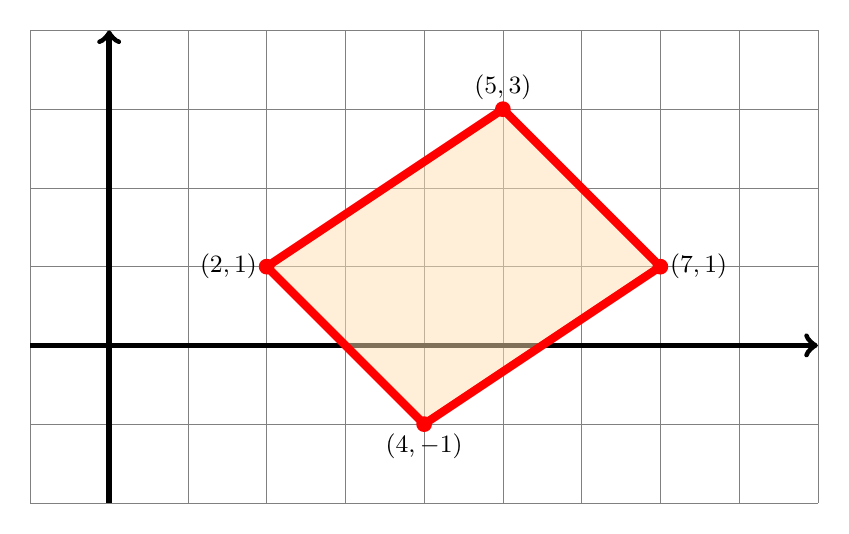
\begin{tikzpicture}
\definecolor{MyYellow}{RGB}{255, 224, 179}
\foreach \x in {-1,...,9}{
\draw[help lines] (\x, -2) -- (\x, 4);
}
\foreach \y in {-2,...,4}{
\draw[help lines] (-1, \y) -- (9, \y);
}
\draw[->, line width = 2pt] (-1,0) -- (9,0);
\draw[->, line width = 2pt] (0,-2) -- (0,4);
\node[anchor =  east] at (2,1) {\small $(2,1)$};
\node[anchor =  south] at (5,3) {\small $(5,3)$};
\node[anchor =  west] at (7,1) {\small $(7,1)$};
\node[anchor =  north] at (4,-1) {\small $(4,-1)$};
\fill[MyYellow, opacity = 0.5] (2, 1) -- (5, 3) -- (7, 1) -- (4, -1) -- cycle;
\foreach \x/\y in {2/1, 5/3, 7/1, 4/-1}{
\fill[red] (\x, \y) circle (0.1);
}
\draw[red,  line width=3, line join=bevel] (2, 1) -- (5, 3) -- (7, 1) -- (4, -1) -- cycle;
\end{tikzpicture} 
\end{equation*}

\newpage


{\bf Example.} Calculate the area of the  triangle with vertices at the points
$(2, 1)$, $(5, 3)$,  $(4, -1)$. 
\vskip 5mm

\begin{equation*}
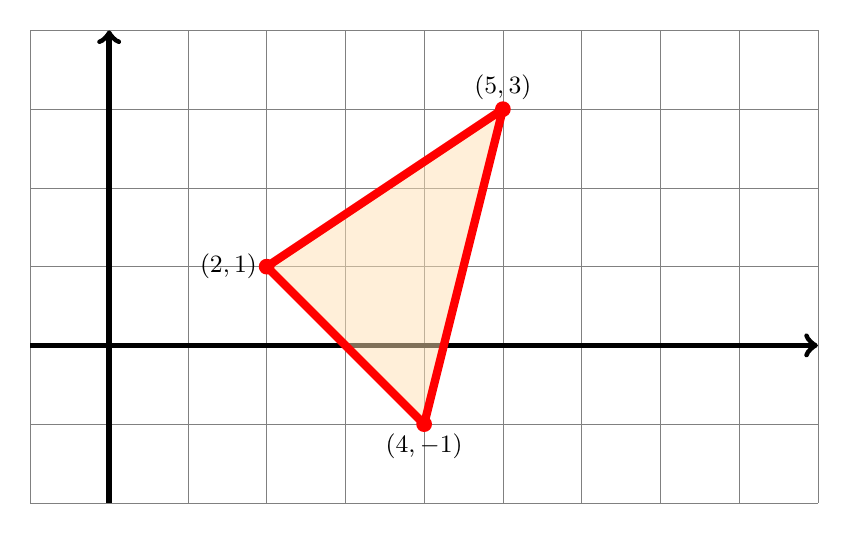
\begin{tikzpicture}
\definecolor{MyYellow}{RGB}{255, 224, 179}
\foreach \x in {-1,...,9}{
\draw[help lines] (\x, -2) -- (\x, 4);
}
\foreach \y in {-2,...,4}{
\draw[help lines] (-1, \y) -- (9, \y);
}
\draw[->, line width = 2pt] (-1,0) -- (9,0);
\draw[->, line width = 2pt] (0,-2) -- (0,4);
\node[anchor =  east] at (2,1) {\small $(2,1)$};
\node[anchor =  south] at (5,3) {\small $(5,3)$};
\node[anchor =  north] at (4,-1) {\small $(4,-1)$};
\fill[MyYellow, opacity = 0.5] (2, 1) -- (5, 3)  -- (4, -1) -- cycle;
\foreach \x/\y in {2/1, 5/3, 4/-1}{
\fill[red] (\x, \y) circle (0.1);
}
\draw[red,  line width=3, line join=bevel] (2, 1) -- (5, 3)  -- (4, -1) -- cycle;
\end{tikzpicture} 
\end{equation*}

\newpage



{\bf Note.}  In order to compute areas of other polygons, subdivide them 
into triangles.
\vskip 5mm

\begin{equation*}
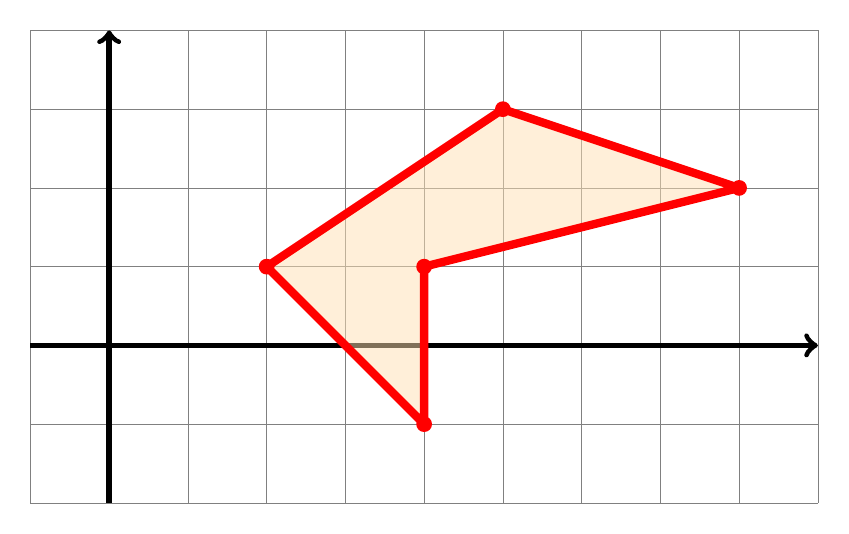
\begin{tikzpicture}
\definecolor{MyYellow}{RGB}{255, 224, 179}
\foreach \x in {-1,...,9}{
\draw[help lines] (\x, -2) -- (\x, 4);
}
\foreach \y in {-2,...,4}{
\draw[help lines] (-1, \y) -- (9, \y);
}
\draw[->, line width = 2pt] (-1,0) -- (9,0);
\draw[->, line width = 2pt] (0,-2) -- (0,4);
\fill[MyYellow, opacity = 0.5] (2, 1) -- (5, 3) -- (8, 2)-- (4, 1) -- (4, -1) -- cycle;
\foreach \x/\y in {2/1, 5/3, 8/2, 4/1, 4/-1}{
\fill[red] (\x, \y) circle (0.1);
}
\draw[red,  line width=3, line join=bevel] (2, 1) -- (5, 3)  -- (8, 2)-- (4, 1) -- (4, -1) -- cycle;
\end{tikzpicture} 
\end{equation*}

\newpage



%---------------------------
%  Part
%---------------------------
\lecture{Determinants and linear transformations}



\underline{\bf Recall:} If $A$ is a $2\times 2$ matrix then it defines a linear transformation
$$T_{A}\colon \R^{2} \to \R^{2} \ \ \ \ \ T_{A}(\vv) = A\vv$$


{\bf Note.} $T_{A}$ maps parallelograms to parallelograms: 


\vskip 10mm

\btikz[
          line1/.style ={line width = 3, ->}
          ]
          
\begin{scope}[scale = 0.8]
\draw[->, line width = 2pt] (-1,0) -- (5,0);
\draw[->, line width = 2pt] (0,-1) -- (0,5);

\draw[fill=black!20] (0,0) -- ++(3,0.5) -- ++(1,3) -- ++(-3, -0.5) -- cycle;
\draw[red, line1] (0,0) -- (3, 0.5) node[pos=1.05, yshift = -3pt, anchor = west] {$\vv_{1}$};
\draw[blue, line1] (0,0) -- (1, 3) node[pos=1.05, anchor = south] {$\vv_{2}$};
\fill[] (0,0) circle (0.09);
\end{scope}

\begin{scope}[scale = 0.8, xshift = 120mm]
\draw[fill=black!20] (0,0) -- ++(2,1) -- ++(-1,3) -- ++(-2, -1) -- cycle;
\draw[red, line1] (0,0) -- (2, 1) node[pos=1.05, yshift = -3pt, anchor = west] {$T_{A}(\vv_{1})$};
\draw[blue, line1] (0,0) -- (-1, 3) node[pos=1.05, anchor = south] {$T_{A}(\vv_{2})$};

\draw[->, line width = 2pt] (-1.5,0) -- (5,0);
\draw[->, line width = 2pt] (0,-1) -- (0,5);
\fill[] (0,0) circle (0.09);
\end{scope}
\etikz


\vskip 10mm

\begin{cbox}[Theorem]
If $A$ is a $2\times 2$ matrix and $\vv_{1}, \vv_{1}\in \R^{2}$ then 
$$\text{area}(T_{A}(\vv_{1}), T_{A}(\vv_{2})) = \left | \det A \right | \cdot \text{area}(\vv_{1}, \vv_{2})$$
\end{cbox}


\newpage

\underline{\bf Generalization:}

\vskip 3mm

\begin{cbox}[Theorem]
If $A$ is a $2\times 2$ matrix then for any region $S$ of $\R^{2}$ we have: 
$$\text{area}(T_{A}(S)) = \left | \det A \right | \cdot \text{area}(S)$$
\end{cbox}

\vskip 10mm

\btikz[
          line1/.style ={line width = 2, ->}
          ]
          
\begin{scope}[scale = 0.8]
\draw[->, line width = 2pt] (-1,0) -- (5,0);
\draw[->, line width = 2pt] (0,-1) -- (0,5);
\draw[line1, fill=black!20] (2.3,2.3) circle (1.7);
\node[anchor = west] at (3.5, 0.75) {S};
\end{scope}

\begin{scope}[scale = 0.8, xshift = 120mm]
\draw[line1, fill=black!20, rotate around = {45:(0,0)}] (3,0) ellipse [x radius= 2.5, y radius= 0.6];
\node[anchor =  west] at (2, 0.75) {$T_{A}(S)$};
\draw[->, line width = 2pt] (-1.5,0) -- (5,0);
\draw[->, line width = 2pt] (0,-1) -- (0,5);

\end{scope}
\etikz


\vskip 10mm

\emph{Idea of the proof.}

\vskip 3mm

The area of $S$ can be approximated by the sum of small squares covering $S$.

\vskip 10mm 

\begin{flushright}
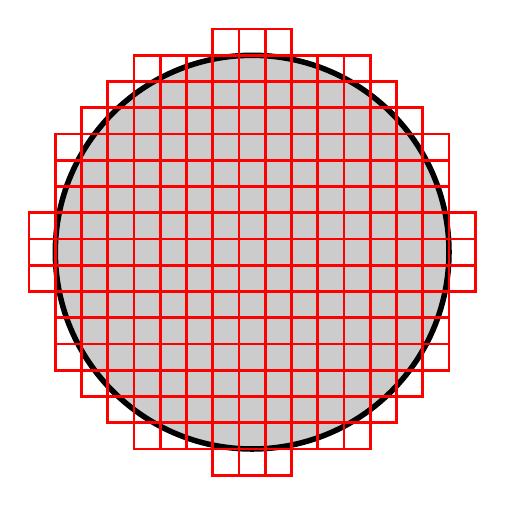
\begin{tikzpicture}[ scale=5,
          line1/.style ={line width = 2, ->},
          line2/.style ={line width = 1}          
          ]

\draw[line1, fill=black!20] (0.5, 0.5) circle (0.5);
\foreach \j in {6, 7,8}{
\draw[line2, red] (-1/15, \j/15) rectangle (-1/15 + 1/15, \j/15 + 1/15);
}
\foreach \j in {3, 4,..., 11}{
\draw[line2, red] (0/15, \j/15) rectangle (0/15 + 1/15, \j/15 + 1/15);
}
\foreach \j in {2, 3,..., 12}{
\draw[line2, red] (1/15, \j/15) rectangle (1/15 + 1/15, \j/15 + 1/15);
}
\foreach \j in {1,2,..., 13}{
\draw[line2, red] (2/15, \j/15) rectangle (2/15 + 1/15, \j/15 + 1/15);
}
\foreach \j in {0,1,..., 14}{
\draw[line2, red] (3/15, \j/15) rectangle (3/15 + 1/15, \j/15 + 1/15);
}
\foreach \j in {0,1,..., 14}{
\draw[line2, red] (4/15, \j/15) rectangle (4/15 + 1/15, \j/15 + 1/15);
}
\foreach \j in {0,1,..., 14}{
\draw[line2, red] (5/15, \j/15) rectangle (5/15 + 1/15, \j/15 + 1/15);
}
\foreach \j in {-1,0,..., 15}{
\draw[line2, red] (6/15, \j/15) rectangle (6/15 + 1/15, \j/15 + 1/15);
}
\foreach \j in {-1,0,..., 15}{
\draw[line2, red] (7/15, \j/15) rectangle (7/15 + 1/15, \j/15 + 1/15);
}
\foreach \j in {-1,0,..., 15}{
\draw[line2, red] (8/15, \j/15) rectangle (8/15 + 1/15, \j/15 + 1/15);
}
\foreach \j in {0,1,..., 14}{
\draw[line2, red] (9/15, \j/15) rectangle (9/15 + 1/15, \j/15 + 1/15);
}
\foreach \j in {0,1,..., 14}{
\draw[line2, red] (10/15, \j/15) rectangle (10/15 + 1/15, \j/15 + 1/15);
}
\foreach \j in {0,1,..., 14}{
\draw[line2, red] (11/15, \j/15) rectangle (11/15 + 1/15, \j/15 + 1/15);
}
\foreach \j in {1,2,..., 13}{
\draw[line2, red] (12/15, \j/15) rectangle (12/15 + 1/15, \j/15 + 1/15);
}
\foreach \j in {2,3,..., 12}{
\draw[line2, red] (13/15, \j/15) rectangle (13/15 + 1/15, \j/15 + 1/15);
}
\foreach \j in {3,4,..., 11}{
\draw[line2, red] (14/15, \j/15) rectangle (14/15 + 1/15, \j/15 + 1/15);
}
\foreach \j in {6,7,8}{
\draw[line2, red] (15/15, \j/15) rectangle (15/15 + 1/15, \j/15 + 1/15);
}
\end{tikzpicture}
\end{flushright}

\newpage

%---------------------------
%  Part
%---------------------------
\lecture{Sign of the determinant}


{\bf Example.}

\vskip 5mm

$
A = 
\bbm
2 & 1 \\
1 & 3  \\
\ebm
$


\vskip 5mm

\btikz[scale = 0.7]
\begin{scope}
\draw[->, line width = 2pt] (-1,0) -- (5,0);
\draw[->, line width = 2pt] (0,-1) -- (0,5);
\end{scope}
\begin{scope}[xshift = 130mm]
\draw[->, line width = 2pt] (-1,0) -- (5,0);
\draw[->, line width = 2pt] (0,-1) -- (0,5);
\end{scope}
\etikz

\vskip 10mm

{\bf Example.}

\vskip 5mm

$
A = 
\bbm
2 & 3 \\
2 & 1  \\
\ebm
$


\vskip 5mm

\btikz[scale = 0.7]
\begin{scope}
\draw[->, line width = 2pt] (-1,0) -- (5,0);
\draw[->, line width = 2pt] (0,-1) -- (0,5);
\end{scope}
\begin{scope}[xshift = 130mm]
\draw[->, line width = 2pt] (-1,0) -- (5,0);
\draw[->, line width = 2pt] (0,-1) -- (0,5);
\end{scope}
\etikz

\vfill

\begin{cbox}[Theorem]
If $A$ is a $2\times 2$ matrix then the linear transformation $T_{A}\colon \R^{2}\to \R^{2}$ preserves
orientation if $\det A > 0$ and reverses orientation if $\det A < 0$. 
\end{cbox}


\newpage

%---------------------------
%  Part
%---------------------------
\lecture{General vector spaces}


\begin{center}
\begin{tabular}{p{0.47\textwidth} !{\vrule width 2pt}  p{0.47\textwidth}}

\begin{minipage}{0.46\textwidth}
\begin{center} 
{\bf Linear Algebra} 
\end{center}
\end{minipage}
 &
\begin{minipage}{0.46\textwidth}
\begin{center} 
{\bf Calculus} 
\end{center}
\end{minipage} 
\\[3mm]
\noalign{\hrule height 2pt}

\begin{minipage}{0.46\textwidth}
$$\R^{n} = 
\begin{pmatrix} 
\text{set of all column vectors} \\
\text{with $n$ entries} \\
\end{pmatrix}
$$
\end{minipage}
&
\hspace{1mm}
\begin{minipage}{0.46\textwidth}
$$C^{\infty}(\R) = 
\begin{pmatrix} 
\text{set of all smooth} \\
\text{functions } f\colon \R \ra \R \\
\end{pmatrix}
$$
\end{minipage} 
\\[15mm]


\begin{minipage}{0.46\textwidth}
{\bf Column vectors} can be added and multiplied 
by real numbers.
\end{minipage}
& 
\hspace{2mm}
\begin{minipage}{0.46\textwidth}
{\bf Functions}  can be added and multiplied 
by real numbers.
\end{minipage}
\\[15mm]


\begin{minipage}{0.46\textwidth}
{\bf Linear transformation} is a function
\vskip -10mm
$$\phantom{C^{\infty}} T\colon \R^{n} \to \R^{m}, \ \ \ T(\vv) = A\vv $$
\vskip -3mm
It satisfies:
\benu
\item[\textbullet] $T(\uu + \vv) = T(\uu) + T(\vv)$
\item[\textbullet] $T(c\vv) = cT(\vv)$
\eenu
\end{minipage}
& 
\hspace{1mm}
\begin{minipage}{0.46\textwidth}
{\bf Differentiation} is a function
\vskip -10mm
$$D\colon C^{\infty}(\R) \to C^{\infty}(\R), \ \ \  D(f) = f' $$
\vskip -3mm
It satisfies:
\benu
\item[\textbullet] $D(f+g) = D(f) + D(g)$
\item[\textbullet] $D(cf) = cD(f)$
\eenu
\end{minipage}
\\[25mm]


\begin{minipage}{0.46\textwidth}
{\bf Typical problem:} given a vector $\bb$
find all vectors $\xx$ such that 
\vskip -4mm
$$T(\xx) = \bb$$
\vskip -3mm
(i.e solve the  equation $A\xx  = \bb$).
\end{minipage}
& 
\hspace{1mm}
\begin{minipage}{0.46\textwidth}
{\bf Typical problem:} given a function  $g$
find all functions $f$ such that 
\vskip -4mm
$$D(f) = g$$
\vskip -3mm
(i.e find antiderivatives of  $g$).
\end{minipage}
\\[25mm]

\begin{minipage}{0.46\textwidth}
{\bf Fact:}  Such vectors $x$ are of the form 
\vskip -4mm
$$\xx = \vv_{0} + \nn$$
\vskip -3mm
where:
\benu
\item[\textbullet] $\vv_{0}$ is some distinguished solution of $A\xx = \bb$;
\item[\textbullet] $\nn\in \Nul(A)$ (i.e. $\nn$ is a solution of $A\xx = \zzero$).
\eenu
\end{minipage}
& 
\hspace{1mm}
\begin{minipage}{0.47\textwidth}
{\bf Fact:} Such functions $f$ are of the form 
\vskip -4mm
$$f = F + C$$
\vskip -3mm
where:
\benu
\item[\textbullet] $F$ is some distinguished antiderivative of $g$;
\item[\textbullet] $C$ is a constant function (i.e. $C$ is a solution of $D(f) = 0$).
\eenu
\end{minipage}

\end{tabular}
\end{center}

\newpage


\begin{cbox}[Definition]
A \emph{(real) vector space} is a set $V$ together with two operations: 

\vskip 3mm

\quad $\bullet$\ addition
$$V\times V \lra V$$
\vskip -10mm
$$\ \ \ \ (\uu, \ \ \vv) \ \longmapsto\  \uu+\vv$$

\quad $\bullet$\ multiplication by scalars
$$\R\times V \lra V$$
\vskip -11mm
$$\ \ \ (c, \ \ \vv) \ \longmapsto\  c\cdot \vv$$

Moreover the following conditions must be satisfied:

\vskip 5mm
 
\begin{itemize}
\item[{\textbf 1)\ }] $\uu+\vv = \vv+\uu$

\vskip 3mm

\item[{\textbf 2)\ }] $(\uu +\vv) +\ww = \uu + (\vv +\ww )$ 

\vskip 3mm

\item[{\textbf 3)\ }] there is an element $\zzero\in V$ such that $\zzero +\uu = \uu$
for any $\uu\in V$

\vskip 3mm

\item[{\textbf 4)\ }] for any $\uu\in V$ there is an element $-\uu \in V$ such that 
$\uu + (-\uu)=\zzero$

\vskip 3mm

\item[{\textbf 5)\ }] $c (\uu+\vv) = c\uu + c\vv$

\vskip 3mm

\item[{\textbf 6)\ }] $(c+d)\uu = c\uu + d\uu$

\vskip 3mm

\item[{\textbf 7)\ }] $(cd)\uu = c(d\uu)$

\vskip 3mm

\item[{\textbf 8)\ }] $1\uu = \uu$

\end{itemize}

\vskip 5mm

Elements of $V$ are called \emph{vectors}.

\end{cbox}

\newpage

\begin{cbox}[Theorem]
If $V$ is a vectors space then:
\begin{itemize}
\item[\textbf{1)\ }] $c\cdot \zzero = \zzero$\ \  where $c\in \R$ and $\zzero \in V$ is the zero vector;

\vskip 3mm

\item[\textbf{2)\ }] $0\cdot \uu = \zzero$\ \  where $0\in \R$, $\uu\in V$ and $\zzero$ is the zero vector;  

\vskip 3mm

\item[\textbf{3)\ }] $(-1)\cdot \uu = -\uu$
\end{itemize}
\end{cbox}

\newpage

{\bf Examples of vector spaces.}


\newpage


%---------------------------
%  Part
%---------------------------
\lecture{Vector subspaces}

\begin{cbox}[Defitnition]
Let $V$ be a vector space. A \emph{subspace} of $V$ is a subset $W\subseteq V$ such that 
\begin{itemize}
\item[\textbf{1)\ }] $\zzero \in W$

\vskip 3mm

\item[\textbf{2)\ }] if $\uu, \vv \in W$ then $\uu + \vv \in W$

\vskip 3mm

\item[\textbf{3)\ }] if $\uu\in W$ and $c\in \R$ then $c\uu\in W$. 
\end{itemize}
\end{cbox}

\vskip 5mm

{\bf Example.} 

\vskip 3mm

Recall: $\Poly = $ the vector space of all polynomials.  

\vfill

\begin{cbox}[Proposition]
Let $V$ be a vector space and $W\subseteq V$ is a subspace then $W$ is itself 
a vector space. 
\end{cbox}


\newpage

{\bf Example.} 

\vskip 3mm

Recall: $\FF(\R) = $ the vector space of all functions $f\colon \R \to \R$

\vskip 10mm

\underline{Some interesting subspaces of $\FF(\R)$:}

\vskip 7mm

{\bf 1)} $C(\R) = $ the subspace of all continuous functions $f\colon \R\to \R$

\vskip 7mm

{\bf 2)} $C^{n}(\R) = $ the subspace of all  functions $f\colon \R\to \R$ that are differentiable $n$ or more times. 

\vskip 7mm

{\bf 3)} $C^{\infty}(\R) = $ the subspace of all  smooth functions $f\colon \R\to \R$ (i.e. functions that have derivatives 
of all orders: $f'$, $f''$, $f'''$, $\dots$).

\newpage

{\bf Note.} If $V$ is a vector space then:

\vskip 3mm

\benu
\item[\bf 1)] the biggest subspace of $V$ is $V$ itself; \\[-4mm]
\item[\bf 2)] the smallest subspace of $V$ is the subspace $\{\zzero\}$ consisting of the zero vector only;\\[-4mm]
\item[\bf 3)] if a subspace of $V$ contains a non-zero vector, then it contains infinitely many vectors. 
\eenu



%---------------------------
%  Part
%---------------------------
\lecture{Linear transformations of vector spaces}



\begin{cbox}[Definition]
Let $V, W$ be vector spaces
A \emph{linear transformation} is  a function 
$$T\colon V \to W$$
which satisfies the following conditions:
\benu
\item[{\bf 1)}] $T(\uu + \vv) = T(\uu) + T(\vv)$ for all $\uu, \vv \in V$ \\[-4mm]
\item[{\bf 2)}] $T(c\vv) = cT(\vv)$ for any $\vv \in V$ and any scalar $c$. 
\eenu
\end{cbox}


\vskip 90mm

%\begin{cbox}[Proposition]
%If $T\colon V \to W$ is a linear transformation then  $T(\zzero) = \zzero$. 
%\end{cbox}


\newpage

{\bf Note.} If  $T\colon V\to W$ is a linear transformation then for any vector $\bb\in W$ we can consider the
equation
$$T(\xx) = \bb$$


\newpage


\begin{cbox}[Definition]
If  $T\colon V \to W$ is a linear transformation then:

\benu
\item[{\bf 1)}] The \emph{kernel} of $T$ is the set 
$$\Ker(T) = \{\vv \in V \ | \ T(\vv) = \zzero\}$$
\item[{\bf 2)}] The \emph{image} of $T$ is the set 
$$\Img(T) = \{\ww \in W \ | \ \ww =  T(\vv) \text{ for some } \vv\in V\}$$
\eenu
\end{cbox}


\newpage

\begin{cbox}[Proposition]
If  $T\colon V \to W$ is a linear transformation then:

\benu
\item[{\bf 1)}]  $\Ker(T)$ is a subspace of $V$ \\[-4mm]
\item[{\bf 2)}]  $\Img(T)$ is a subspace of $W$
\eenu
\end{cbox}

\vskip 50mm


\begin{cbox}[Theorem]
If  $T\colon V \to W$ is a linear transformation and $v_{0}$ is a solution of the equation 
$$T(\xx) = \bb$$
then all other solutions of this equation are vectors of the form 
$$\vv = \vv_{0} + \nn$$
where $\nn \in \Ker(T)$. 
\end{cbox}


\newpage

{\bf Example.}

$$D \colon C^{\infty}(\R) \lra C^{\infty}(\R)$$
$$\ \ \ \ f \ \ \longmapsto \ \ f'$$





%---------------------------
%  Part
%---------------------------
\lecture{Basis of a vector space}

\underline{\bf Recall:}

\vskip 5mm

{\textbullet} A vector space is a set $V$ equipped with operations of addition and multiplication by scalars. 
These operations must satisfy some properties. 

\vskip 5mm

{\textbullet} Some examples of vector spaces:

\vskip 5mm

\benu
\item[\bf 1)] $\R^{n} = $  the vector space of column vectors.\\[-2mm]
\item[\bf 2)] $\FF(\R) = $ the vector space of all functions $f\colon \R\to \R$. \\[-2mm]
\item[\bf 3)] $C(\R) = $ the vector space of all continuous functions $f\colon \R\to \R$. \\[-2mm]
\item[\bf 4)] $C^{\infty}(\R) = $ the vector space of all smooth functions $f\colon \R\to \R$. \\[-2mm]
\item[\bf 5)] $M_{m, n}(\R) = $ the vector space of all $m\times n$ matrices. \\[-2mm]
\item[\bf 6)] $\Poly = $ the vector space of all polynomials.   \\[-2mm]
\item[\bf 7)] $\Poly_{n} = $ the vector space of polynomials of degree $\leq n$.  
\eenu


\vskip 5mm

{\textbullet}  If $V$, $W$ are vector spaces then a linear transformation is a function $T\colon V \to W$ such that 

\vskip 5mm

\benu
\item[\bf 1)] $T(\uu + \vv) = T(\uu) + T(\vv)$ \\[-2mm]
\item[\bf 2)] $T(c\vv) = cT(\vv)$ \\[-2mm]
\eenu


\vskip 5mm



{\textbullet}  Many problems involving $\R^{n}$ can be easily solved using row reduction, 
matrix multiplication etc. 

\vskip 5mm

{\textbullet} The same types of problems involving other vector spaces can be difficult to solve. 


\newpage

\underline{\bf Next goal:} 

\vskip 5mm

If $V$ is a \emph{finite dimensional} vector space then we can construct 
a \emph{coordinate mapping} 
$$V \to \R^{n}$$
which lets us turn computations in $V$ into computations in $\R^{n}$.

\vskip 20mm


\btikz[scale = 1.1, 
          line1/.style ={line width = 2pt, red, text=black},
          line2/.style  ={red!30, line width = 16},
          line3/.style  = {red!30, line width = 16, ->, >={Triangle[length = 14pt, width = 24pt ]}}, 
          line4/.style  = {white, line width = 20, ->, >={Triangle[length = 14pt, width = 24pt ]}}
          ]

\draw[line2, text=red] ([shift=(120:2.5)] 1.5, -1.25) arc(120:240:3.2 and 2.5);
\draw[line2,  text=red] ([shift=(-60:2.5)] 1.5, -1.25) arc(-60:70: 3.2 and 2.5);

\draw[line4, text=red] ([shift=(120:2.5)] 1.5, -1.25) arc(120:184:3.2 and 2.5);
\draw[line4,  text=red] ([shift=(-60:2.5)] 1.5, -1.25) arc(-60:9: 3.2 and 2.5);

\draw[line3, text=red] ([shift=(120:2.5)] 1.5, -1.25) arc(120:180:3.2 and 2.5); 
\draw[line3,  text=red] ([shift=(-60:2.5)] 1.5, -1.25) arc(-60:5: 3.2 and 2.5);

\draw[line1, fill=white] (0,0) rectangle +(3,1.5) node[pos=0.5] {\small \begin{tabular}{c} $V$ \\ vector space \end{tabular}};

\draw[line1, fill = white] (0,-4) rectangle +(3,1.5) node[pos=0.5] {\small \begin{tabular}{c} $\R^{n}$ \\ \end{tabular}};

\node[red] at (-3, -1.25)
{\begin{minipage}{25mm}
\begin{flushright}
\emph{
coordinate \\
mapping
}
\end{flushright}
\end{minipage}
};
\node[red] at (6, -1.25)
{\begin{minipage}{25mm}
\emph{
inverse \\
coordinate \\
mapping
}
\end{minipage}
};
\etikz



\newpage

\begin{center}
\bf{Motivation: How to assign coordinates to vectors}
\end{center}

\vskip -10mm

\btikz [line1/.style = {red, line width = 3, ->}]

\draw[line width = 1.2pt] (0, 0) rectangle (\textwidth, 8);
\draw[line1] (0.5*\textwidth,3) -- +(2, 1) node[pos=0.5, anchor = south east] {$\vv$};
\fill[red] (0.5*\textwidth,3) circle (0.1);
\
\etikz

\vskip -12mm

\btikz [line1/.style = {red, line width = 3, ->}]

\draw[line width = 1.2pt] (0, 0) rectangle (\textwidth, 8);
\draw[line1] (0.5*\textwidth,3) -- +(2, 1) node[pos=0.5, anchor = south east] {$\vv$};
\fill[red] (0.5*\textwidth,3) circle (0.1);
\
\etikz

\newpage

\begin{cbox}[Definition]
If $V$ is a vector space then  vector $\ww\in V$ is a \emph{linear combination} of vectors $\vv_{1}, \dots \vv_{p}\in V$
if there exist scalars $c_{1}, \dots, c_{p}$ such that
$$\ww = c_{1}\vv_{1} + {\dots} + c_{p}\vv_{p}$$ 

\end{cbox}


\vskip 5mm

\begin{cbox}[Definition]
If $V$ is a vector space and $\vv_{1}, {\dots}, \vv_{p}$ are vectors in $V$ then 
$$\Span(\vv_{1}, {\dots}, \vv_{p})
= 
\left\{
\begin{matrix}
\text{the set of all} \\
\text{linear combinations} \\
c_{1}\vv_{1} + {\dots} + c_{p}\vv_{p} \\
\end{matrix}
\right\}
$$
\end{cbox}


\vskip 5mm

\begin{cbox}[Definition]
If $V$ is a vector space and $\vv_{1}, {\dots}, \vv_{p}$ are vectors in $V$ such that 
$$ V = \Span(\vv_{1}, {\dots}, \vv_{p})$$
the the set $\{\vv_{1}, \dots , \vv_{p} \}$ is called the \emph{spanning set} of $V$. 
\end{cbox}

\newpage

{\bf Example.}

\newpage

\begin{cbox}[Definition]
If $V$ is a vector space and $\vv_{1}, {\dots}, \vv_{p} \in V$
then the set $\{\vv_{1}, \dots , \vv_{p} \}$ is \emph{linearly independent}
if the homogenous equation 
$$x_{1}\vv_{1} + {\dots} + x_{p}\vv_{p} = \zzero$$
has only one, trivial solution $x_{1} = 0, \dots, x_{p} = 0$. Otherwise the set is \emph{linearly dependent}.
\end{cbox}

\vskip 5mm

\begin{cbox}[Theorem]
Let $V$ be a vector space, and let $\vv_{1}, \dots, \vv_{p}\in V$. If the set  $\{\vv_{1}, \dots, \vv_{p} \}$ 
is  linearly independent then the equation
$$x_{1}\vv_{1} + {\dots} + x_{p}\vv_{p} = \ww$$
has exactly one solution for any vector $\ww \in \Span(\vv_{1}, \dots, \vv_{p})$. 
\end{cbox}


\newpage

{\bf Example.}

\vskip 5mm

Recall: $\FF(\R) = $ the vector space of all functions $f\colon \R\to \R$. Let $f, g, h\in \FF(\R)$ be the following 
functions:
$$f(t) = \sin(t), \ \ \ g(t) = \cos(t), \ \ \ h(t) = \cos^{2}(t)$$
Check if the set $\{f, g, h\}$ is linearly independent. 

\newpage


{\bf Example.}

\vskip 5mm

Let $f, g, h\in \FF(\R)$ be the following functions:
$$f(t) = \sin^{2}(t), \ \ \ g(t) = \cos^{2}(t), \ \ \ h(t) = \cos 2t$$
Check if the set $\{f, g, h\}$ is linearly independent. 

\newpage


\begin{cbox}[Definition]
A \emph{basis} of a vector space $V$ is an ordered set of vectors
$$\BB = \{\bb_{1}, {\dots}, \bb_{n}\}$$
such that 
\benu
\item[\bf 1)]  $\Span(\bb_{1}, {\dots}, \bb_{n}) = V$ \\[-4mm]
\item[\bf 2)]  The set $\{\bb_{1}, {\dots}, \bb_{n}\}$ is linearly independent. 
\eenu
\end{cbox}

\newpage

\begin{cbox}[Theorem]
A set $\BB = \{\bb_{1}, {\dots}, \bb_{n}\}$ is a basis of a vector space $V$ if any only if
for each $\vv\in V$ the vector equation 
$$x_{1}\bb_{1} + {\dots} + x_{n}\bb_{n} = \vv$$
has a unique solution. 
\end{cbox}


\vfill

\begin{cbox}[Definition]
Let $\BB = \{\bb_{1}, {\dots}, \bb_{n}\}$ be a basis of a vector space $V$. 
For  $\vv\in V$ let $c_{1}, \dots, c_{n}$ be the unique numbers such that 
$$c_{1}\bb_{1} + {\dots} + c_{n}\bb_{n} = \vv$$
Then the vector
$$
\begin{bmatrix}
c_{1} \\
\vdots \\
c_{n}  \\
\end{bmatrix}
\in \R^{n}
$$
is called the \emph{coordinate vector of $\vv$ relative to the basis $\BB$} and it is denoted by 
$\begin{bmatrix}\vv\end{bmatrix}_{\BB}$. 
\end{cbox}

\newpage

{\bf Example.} Let $\EE = \{1, t, t^{2}\}$ be the standard basis of $\Poly_{2}$, and let 
$$p(t) = 3+2t -4t^{2}$$
Find the coordinate vector $\begin{bmatrix}p\end{bmatrix}_{\EE}$. 

\vskip 70mm

{\bf Example.} Let $\BB = \{1, 1+t, 1+t+t^{2}\}$. One can check that $\BB$ is a basis of $\Poly_{2}$. Let 
$$p(t) = 3+2t -4t^{2}$$
Find the coordinate vector $\begin{bmatrix}p\end{bmatrix}_{\BB}$. 


%---------------------------
%  Part
%---------------------------
\lecture{Dimension of a vector space}

\underline{\bf Recall:}

\vskip 5mm

{\textbullet\ } A basis of a vector space $V$ is a set of vectors $\BB = \{\bb_{1}, {\dots}, \bb_{n}\}$ such that
\benu
\item[\bf 1)]  $\Span(\bb_{1}, {\dots}, \bb_{n}) = V$ \\[-4mm]
\item[\bf 2)]  The set $\{\bb_{1}, {\dots}, \bb_{n}\}$ is linearly independent. 
\eenu


\vskip 70mm

{\textbullet\ } 
For  $\vv\in V$ let $c_{1}, \dots, c_{n}$ be the unique numbers such that 
$$c_{1}\bb_{1} + {\dots} + c_{n}\bb_{n} = \vv$$
The vector
$$
\begin{bmatrix}\vv\end{bmatrix}_{\BB} = 
\begin{bmatrix}
c_{1} \\
\vdots \\
c_{n}  \\
\end{bmatrix}
\in \R^{n}
$$
is called the \emph{coordinate vector of $\vv$ relative to the basis $\BB$}.

\newpage


\ 

\vskip 10mm

\btikz[scale = 1.1, 
          line1/.style ={line width = 2pt, red, text=black},
          line2/.style  ={red!30, line width = 16},
          line3/.style  = {red!30, line width = 16, ->, >={Triangle[length = 14pt, width = 24pt ]}}, 
          line4/.style  = {white, line width = 20, ->, >={Triangle[length = 14pt, width = 24pt ]}}
          ]

\draw[line2, text=red] ([shift=(120:2.5)] 1.5, -1.25) arc(120:240:3.2 and 2.5);
\draw[line2,  text=red] ([shift=(-60:2.5)] 1.5, -1.25) arc(-60:70: 3.2 and 2.5);

\draw[line4, text=red] ([shift=(120:2.5)] 1.5, -1.25) arc(120:184:3.2 and 2.5);
\draw[line4,  text=red] ([shift=(-60:2.5)] 1.5, -1.25) arc(-60:9: 3.2 and 2.5);

\draw[line3, text=red] ([shift=(120:2.5)] 1.5, -1.25) arc(120:180:3.2 and 2.5); 
\draw[line3,  text=red] ([shift=(-60:2.5)] 1.5, -1.25) arc(-60:5: 3.2 and 2.5);

\draw[line1, fill=white] (0,0) rectangle +(3,1.5) node[pos=0.5] {\small \begin{tabular}{c} $V$ \\ vector space \end{tabular}};

\draw[line1, fill = white] (0,-4) rectangle +(3,1.5) node[pos=0.5] {\small \begin{tabular}{c} $\R^{n}$ \\ \end{tabular}};

\node[red] at (-3, -1.25)
{\begin{minipage}{25mm}
\begin{flushright}
\emph{
coordinate \\
mapping
}
\end{flushright}
\end{minipage}
};
\node[red] at (6, -1.25)
{\begin{minipage}{25mm}
\emph{
inverse \\
coordinate \\
mapping
}
\end{minipage}
};
\etikz


\vfill

\begin{cbox}[Theorem]
Let $\BB$ be a basis of a vector space $V$. If $\vv_{1}, \dots \vv_{p}, \ww \in V$ then:

\vskip 5mm

\benu
\item[\bf 1)] Solutions of the equation  $x_{1}\vv_{1} + {\dots} + x_{p}\vv_{p} = \ww$
are the same as solutions of the equation 
$x_{1}\begin{bmatrix}\vv_{1}\end{bmatrix}_{\BB} + {\dots} + x_{p}\begin{bmatrix}\vv_{p}\end{bmatrix}_{\BB} = 
\begin{bmatrix}\ww\end{bmatrix}_{\BB}$.\\[3mm]

\item[\bf 2)]  The set of vectors $\{\vv_{1}, \dots \vv_{p}\}$ is linearly independent if and only if the set 
$\left\{ \begin{bmatrix}\vv_{1}\end{bmatrix}_{\BB} , \dots , \begin{bmatrix}\vv_{p}\end{bmatrix}_{\BB}  \right\}$
is linearly independent. \\[3mm]

\item[\bf 3)] $\Span(\vv_{1}, \dots, \vv_{p}) = V$ if any only if 
$\Span\left(\begin{bmatrix}\vv_{1}\end{bmatrix}_{\BB}, \dots, \begin{bmatrix}\vv_{p}\end{bmatrix}_{\BB}\right) = \R^{n}$. 
\\[3mm]

\item[\bf 4)] $\{\vv_{1}, \dots, \vv_{p}\}$ is a basis of $V$ if and only if
$\left\{ \begin{bmatrix}\vv_{1}\end{bmatrix}_{\BB} , \dots , \begin{bmatrix}\vv_{p}\end{bmatrix}_{\BB}  \right\}$
is a basis of $\R^{n}$.
\eenu
\end{cbox}



\newpage


{\bf Example.} Recall that $\Poly_{2}$ is the vector space of polynomials of degree $\leq 2$. 
Consider the following polynomials in $\Poly_{2}$:
\begin{xalignat*}{1}
p_{1}(t) = 1 + 2t + t^{2}   \\
p_{2}(t) = 3 + t + 2t^{2}  \\
p_{3}(t) = 1 -  8t   - t^{2}\\
\end{xalignat*}

\vskip -10mm

Check if the set $\{p_{1}, p_{2}, p_{3}\}$ is linearly independent. 


\newpage

\begin{cbox}[Theorem]
Let $\{\vv_{1}, \dots, \vv_{p}\}$ be vectors in $\R^{n}$. The set $\{\vv_{1}, \dots, \vv_{p}\}$ is a basis of $\R^{n}$
if and only if the matrix 
$$A = \bbm \vv_{1} & \dots & \vv_{p} \\ \ebm$$ 
has a pivot position in every row and in every column (i.e. if $A$ is an invertible matrix).  
\end{cbox}


\vfill

\begin{cbox}[Corollary]
Every basis of $\R^{n}$ consists of $n$ vectors. 
\end{cbox}


\newpage

\begin{cbox}[Theorem]
Let $V$ be a vector space. If $V$ has a basis consisting of $n$ vectors then every basis of $V$ consists of 
$n$ vectors. 
\end{cbox}


\vfill

\begin{cbox}[Definition]
A vector space has \emph{dimension $n$} if $V$ has a basis consisting of  $n$ vectors.  Then we write $\dim V = n$. 
\end{cbox}


\newpage

{\bf Example.}

\newpage


\begin{cbox}[Theorem]
Let $V$ be a vector space such that $\dim V = n$, and let $\vv_{1}, \dots \vv_{p}\in V$. 

\vskip 3mm

{\bf 1)} If $\{\vv_{1}, \dots, \vv_{p}\}$ is a spanning set of $V$ then $p\geq n$. 

\vskip 4mm

{\bf 2)}  If $\{\vv_{1}, \dots, \vv_{p}\}$ is a linearly independent set then $p\leq n$. 
 
\end{cbox}


\vskip 80mm

\begin{cbox}[Corollary]
Let $V$ be a vector space such that $\dim V = n$. If  $W$ be a subspace of $V$ then $\dim W \leq n$. 
Moreover, if $\dim W = n$ then $W = V$. 
\end{cbox}


\newpage

{\bf Note.}

\vskip 2mm 

{\bf 1) } One can show that every vector space has a basis. 

\vskip 3mm

{\bf 2) } Some vector spaces have bases consisting of infinitely many vectors. If $V$ is such vector space 
then we write $\dim V = \infty$. 

\vskip 10mm

{\bf Example.}



%---------------------------
%  Part
%---------------------------
\lecture{The rank theorem}


\underline{\bf Recall:}

\vskip 4mm

If $A   = \bbm \vv_{1} & {\dots}  & \vv_{n} \\ \ebm$ is an $m\times n$ matrix then:

\vskip 4mm  

\benu 
\item[\bf 1)]  $\Col(A) = \Span(\vv_{1}, \dots, \vv_{n})$ \\[-4mm]
\item[\bf 2)]  $\Nul(A) = \{\vv\in \R^{m} \ | \ A\vv = \zzero \}$ \\[-4mm]
\eenu


\newpage

\underline{\bf Construction of a basis of $\Col(A)$}


\vskip 50mm


\begin{cbox}[Lemma]
Let $V$ be a vector space, and let $\vv_{1}, \dots, \vv_{p}\in V$. If a vector 
$\vv_{i}$ is a linear combination of the other vectors then 
$$\Span(\vv_{1}, \dots, \vv_{p}) = \Span(\vv_{1}, \dots, \vv_{i-1}, \vv_{i+1}, \dots, \vv_{p})$$
\end{cbox}

\vskip 10mm

{\bf Upshot.} One can construct a basis of a vector space $V$ as follows:

\vskip 4mm

\benu 
\item[\textbullet] Start with a set of vectors $\{\vv_{1}, \dots, \vv_{p}\}$ such that 
$\Span(\vv_{1}, \dots, \vv_{p}) = V$. \\[-2mm]
\item[\textbullet] Keep removing vectors without changing the span, until you get 
a linearly independent set.  
\eenu


\newpage

{\bf Example.} Find a basis of $\Col(A)$ where $A$ is the following matrix:

\vskip 5mm

$$
A = 
\bbm
1 & 0 & 2 & 0 &  1 & 0 \\
0 & 1 & 3 & 0 & -1 & 0 \\
0 & 0 & 0 & 1 &  3 & 0 \\
0 & 0 & 0 & 0 &  0 & 1 \\
0 & 0 & 0 & 0 &  0 & 0 \\
\ebm
$$


\newpage


{\bf Example.} Find a basis of $\Col(A)$ where $A$ is the following matrix:

\vskip 5mm

$$
A = 
\bbm
-3 &  6 & -1 &  1 &  -7  \\
 1 & -2 &  2 &  3 &  -1  \\
 2 & -4 &  5 &  8 &  -4  \\
\ebm
$$



\newpage


\underline{\bf Construction of a basis of $\Nul(A)$}


\vskip 10mm

{\bf Example.} Find a basis of $\Nul(A)$ where $A$ is the following matrix:

\vskip 5mm

$$
A = 
\bbm
-3 &  6 & -1 &  1 &  -7  \\
 1 & -2 &  2 &  3 &  -1  \\
 2 & -4 &  5 &  8 &  -4  \\
\ebm
$$

\newpage


{\bf Upshot.} If $A$ is matrix then: 

\vskip 3mm

\benu
\item[] $\dim \Col(A) = $ the number of pivot columns of $A$ \\[-4mm]
\item[] $\dim \Nul(A) = $ the number of non-pivot columns of $A$
\eenu

\vskip 5mm

\begin{cbox}[Definition]
If $A$ is a matrix then:

\vskip 3mm

\benu
\item[\textbullet] the dimension of $\Col(A)$ is called the \emph{rank} of $A$ and it is denoted $\rank(A)$ \\[-4mm]

\item[\textbullet] the dimension of $\Nul(A)$ is called the \emph{nullity} of $A$. 
\eenu
\end{cbox}

\vskip 40mm

\begin{cbox}[The Rank Theorem]
If $A$ is an $m\times n$ matrix then 
$$\rank(A) + \dim \Nul(A) = n$$
\end{cbox}


\newpage

{\bf Example.} Let $A$ be a $100\times 101$ matrix such that $\dim \Nul(A) = 1$. Show that 
the equation $A\xx = \bb$ has a solution for each $\bb\in \R^{100}$.


\newpage

{\bf Example.} Let $A$ be a $5\times 9$. Can the null space of $A$ have dimension 3?


%---------------------------
%  Part
%---------------------------
\lecture{Change of basis}

\underline{\bf Recall:} Any basis $\BB = \{\bb_{1}, \dots, \bb_{n} \}$ of a vector space $V$ defines 
a coordinate system:

\vskip -5mm


\btikz
\node[anchor = base] at (0,0)
{\begin{minipage}{100mm}
\begin{center}
$$\vv = c_{1}\bb_{1} + {\dots} + c_{n}\bb_{n} = \vv$$
\end{center}
\end{minipage}
};

\node[single arrow, draw,  minimum height = 10mm, minimum width = 20mm, anchor = tail,
single arrow head extend= 0.5mm,  single arrow tip angle = 130, text height=2ex, text depth=1ex, 
 line width = 2pt, red, text = red,  shape border rotate = 270]  
at (0, -1) {}; 

\node[anchor = base] at (0,-4)
{\begin{minipage}{100mm}
$$\begin{bmatrix}\vv\end{bmatrix}_{\BB} = 
\begin{bmatrix}
c_{1} \\
\vdots \\
c_{n}  \\
\end{bmatrix}
$$
\end{minipage}
};
\etikz


\vskip 10mm

\btikz [line1/.style = {red, line width = 3, ->}]
\coordinate (O) at (0.4*\textwidth,3);
\draw[line width = 1.2pt] (0, 0) rectangle (\textwidth, 10);
\draw[line1] (O) -- +(4, 4) node[pos=0.5, anchor = south east] {$\vv$};
\draw[line1, blue] (O) -- +(-1, 2) node[pos=0.8,  anchor =  east] {$\bb_{1}$};
\draw[line1, blue] (O) -- +(2, 0) node[pos=1, anchor = north] {$\bb_{2}$};
\fill[black] (O) circle (0.1);
\
\etikz


\newpage

{\bf Note.} Choosing a convenient basis can simplify computations. 

\vskip 5mm

{\bf Example.} Graphene lattice.

\begin{equation*}
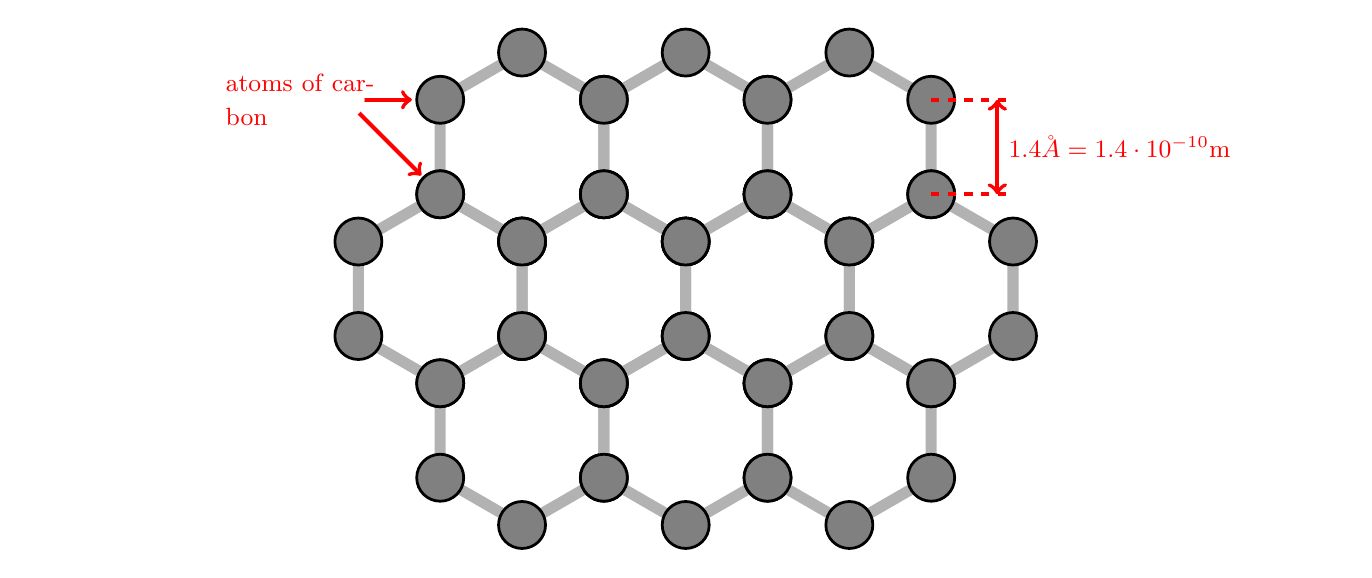
\begin{tikzpicture}[
			     scale = 1.2, 
			     myline/.style={line width = 4pt, color = black!30}, 
			     c/.style={insert path={node[circle, inner sep= 6pt, fill = black!50, draw = black, line width = 1pt] {}}}
			     ]

\draw[line width = 0, opacity = 0] ({-3.5- sin(60)} , 0) -- ({3.5+ 7*sin(60)},0); % just for positioning of the plot

\foreach \i in {0,1,2}{
	\draw[myline] ({\i*2*sin(60)},0) [c] -- ++(90:1) [c] -- ++(30:1) [c] -- ++(-30:1) [c] -- ++(-90:1) [c] -- ++(210:1) [c] -- cycle; 
        \draw[myline] ({\i*2*sin(60)},-3) [c] -- ++(90:1) [c] -- ++(30:1) [c] -- ++(-30:1) [c] -- ++(-90:1) [c] -- ++(210:1) [c] -- cycle; 
	}
\foreach \i in {0,1,2,3}{
	\draw[myline] ({(\i*2-1)*sin(60) } ,-1.5) [c] -- ++(90:1) [c] -- ++(30:1) [c] -- ++(-30:1) [c] -- ++(-90:1) [c] -- ++(210:1) [c] -- cycle; 
	}

\draw[red, dashed, line width = 1.5pt] ({6*sin(60)},0) -- ({6*sin(60) + 0.8},0) ({6*sin(60)},1) -- ({6*sin(60) + 0.8},1);
\draw[red, <->, line width = 1.5pt]  ({6*sin(60) + 0.7},0) -- node[anchor= west] {\small $1.4 {\text \AA} = 1.4\cdot 10^{-10}$m}({6*sin(60) + 0.7},1);

\draw[red,  ->, line width = 1.5pt] (-1,1) -- (-0.3, 1);
\draw[red,  ->, line width = 1.5pt] (-1, 1) -- +(0.8, -0.8); 
\fill[white] (-1, 1) circle (0.2);
\node[red, anchor = east, text width = 20mm] at (-0.5, 1) {\small atoms of carbon}; 
\end{tikzpicture}
\end{equation*}


\begin{figure}[h] %  figure placement: here, top, bottom, or page
   \centering
   \includegraphics[width=3in]{graphene.pdf} 
\end{figure}
\ 
\vskip -20mm \ 
\begin{center}
\emph{Image of graphene taken with an atomic force microscope. 
\\ \textcopyright \ University of Augsburg, Experimental Physics IV.}
\end{center}




\newpage


\begin{center}
\underline{\bf Coordinates of atoms in the graphene lattice}
\end{center}

\vskip 0 mm

\begin{equation*}
\begin{tikzpicture}[
			     scale = 2.0, 
			     myline/.style={line width = 4pt, color = black!30}, 
			     c/.style={insert path={node[circle, inner sep= 6pt, fill = black!50, draw = black, line width = 1pt] {}}}
			     ]
\begin{scope}
\clip (-0.5, -1) rectangle (3.8,3.3);
\foreach \i in {0,..., 5}{
	\draw[help lines] ({\i/1.4}, -1) -- ({\i/1.4}, 3.5);
}
\foreach \i in {-1,..., 4}{
	\draw[help lines] (-0.5, {\i/1.4}) -- ({4*sin(60) + 0.5}, {\i/1.4});
}
\end{scope}
\node[preaction={fill, white}, anchor = east, xshift = -10pt] at (0,0) {\footnotesize $[0,0]$};
\node[preaction={fill, white}, anchor = east, xshift = -10pt] at (0,1) {\footnotesize $[0, 1.4]$};
\node[preaction={fill, white}, anchor = north east, xshift = -10pt] at ({cos(-30)}, {sin(-30)}) {\footnotesize $[1.21, -0.7]$};
\node[preaction={fill, white}, anchor = north west, xshift = 10pt] at ({3*cos(-30)}, {sin(-30)}) {\footnotesize $[3.63, -0.7]$};
\node[preaction={fill, white}, anchor =  east, xshift = -10pt] at ({cos(30)}, {1+ sin(30)}) {\footnotesize $[1.21, 2.1]$};
\node[preaction={fill, white}, anchor =  east, xshift = -10pt] at ({cos(30)}, {2+ sin(30)}) {\footnotesize $[1.21, 3.5]$};
\node[preaction={fill, white}, anchor =  west, xshift = 10pt] at ({2*cos(30)}, 0) {\footnotesize $[2.42, 0]$};
\node[preaction={fill, white}, anchor =  west, xshift = 10pt] at ({2*cos(30)}, 1) {\footnotesize $[2.42, 1.4]$};
\node[preaction={fill, white}, anchor =  west, xshift = 10pt] at ({2*cos(30)}, {2+ 2*sin(30)}) {\footnotesize $[2.42, 4.2]$};
\node[preaction={fill, white}, anchor =  west, xshift = 10pt] at ({3*cos(30)}, {1+ sin(30)}) {\footnotesize $[3.63, 2.1]$};
\node[preaction={fill, white}, anchor =  west, xshift = 10pt] at ({3*cos(30)}, {2+ sin(30)}) {\footnotesize $[3.63, 3.5]$};
\draw[myline] ({sin(60)},1.5) [c] -- ++(90:1) [c] -- ++(30:1) [c] -- ++(-30:1) [c] -- ++(-90:1) [c] -- ++(210:1) [c] -- cycle; 
\foreach \i in {0,1}{
	\draw[myline] ({(\i*2)*sin(60) } ,0) [c] -- ++(90:1) [c] -- ++(30:1) [c] -- ++(-30:1) [c] -- ++(-90:1) [c] -- ++(210:1) [c] -- cycle; 
	}

\draw[->, red, line width = 5pt, >={Triangle[length = 10pt, width = 12pt]}] (0,0) -- ({1/1.4}, 0);
\draw[->, blue, line width = 5pt, >={Triangle[length = 10pt, width = 12pt]}] (0,0) -- (0, {1/1.4});
\fill[black] (0,0) circle (0.07);

\node[text width=5cm, anchor = north west] at (-4,3.2) {\normalsize
In the standard  basis $\EE = \{ \ee_{1}, \ee_{2} \}$:

\ 

$\ee_{1} = 
\bbm
1 \\
0
\ebm
$

\ 

$\ee_{2}= 
\bbm
0 \\
1
\ebm
$

};
\end{tikzpicture}
\end{equation*}






\begin{equation*}
\begin{tikzpicture}[
			     scale = 2.0, 
			     myline/.style={line width = 4pt, color = black!30}, 
			     c/.style={insert path={node[circle, inner sep= 6pt, fill = black!50, draw = black, line width = 1pt] {}}}
			     ]
			     
\begin{scope}
\clip (-0.5, -1.1) rectangle (3.8,3.3);
\foreach \i in {0,..., 4}{
	\draw[help lines] (0, \i) -- +(-30:5);
	\draw[help lines] (0, \i) -- +(150:1);
}
\foreach \i in {-2,..., 2}{
	\draw[help lines] (0, \i) -- +(30:5);
        \draw[help lines] (0, \i) -- +(210:1);
}
\end{scope}
\node[anchor = east, xshift = -10pt] at (0,0) {\footnotesize $[0,0]$};
\node[anchor = east, xshift = -10pt] at (0,1) {\footnotesize $[-1, 1]$};
\node[preaction={fill, white}, anchor = north east, xshift = -10pt] at ({cos(-30)}, {sin(-30)}) {\footnotesize $[1, 0]$};
\node[preaction={fill, white},  anchor = north west, xshift = 10pt] at ({3*cos(-30)}, {sin(-30)}) {\footnotesize $[2, 1]$};
\node[anchor =  east, xshift = -10pt] at ({cos(30)}, {1+ sin(30)}) {\footnotesize $[-1, 2]$};
\node[anchor =  east, xshift = -10pt] at ({cos(30)}, {2+ sin(30)}) {\footnotesize $[-2, 3]$};
\node[anchor =  west, xshift = 10pt] at ({2*cos(30)}, 0) {\footnotesize $[1, 1]$};
\node[anchor =  west, xshift = 10pt] at ({2*cos(30)}, 1) {\footnotesize $[0, 2]$};
\node[anchor =  west, xshift = 10pt] at ({2*cos(30)}, {2+ 2*sin(30)}) {\footnotesize $[-2, 4]$};
\node[anchor =  west, xshift = 10pt] at ({3*cos(30)}, {1+ sin(30)}) {\footnotesize $[0,3]$};
\node[anchor =  west, xshift = 10pt] at ({3*cos(30)}, {2+ sin(30)}) {\footnotesize $[-1, 4]$};

\draw[myline] ({sin(60)},1.5) [c] -- ++(90:1) [c] -- ++(30:1) [c] -- ++(-30:1) [c] -- ++(-90:1) [c] -- ++(210:1) [c] -- cycle; 
\foreach \i in {0,1}{
	\draw[myline] ({(\i*2)*sin(60) } ,0) [c] -- ++(90:1) [c] -- ++(30:1) [c] -- ++(-30:1) [c] -- ++(-90:1) [c] -- ++(210:1) [c] -- cycle; 
	}


\draw[->, red, line width = 5pt, >={Triangle[length = 10pt, width = 12pt]}] (0,0) -- ({cos(-30)}, {sin(-30)});
\draw[->, blue, line width = 5pt, >={Triangle[length = 10pt, width = 12pt]}] (0,0) -- ({cos(30)}, {sin(30)});
\fill[black] (0,0) circle (0.07);

\node[text width=5cm, anchor = north west] at (-4,3.2) {\normalsize
In a more convenient basis $\BB = \{ \bb_{1}, \bb_{2} \}$:

\ 

$\bb_{1} = 
\bbm
1.21 \\
- 0.7
\ebm
$

\ 

$\bb_{2}= 
\bbm
1.21 \\
\phantom{-}0.7
\ebm
$

};

\end{tikzpicture}
\end{equation*}




\newpage


{\bf Problem} Let 
$$\BB= \{\bb_{1}, \dots, \bb_{n}\}, \ \ \ \  \DD = \{\dd_{1}, \dots, \dd_{1}\}$$ 
be two bases  of a vector space $V$, and let $\vv\in V$.  Assume that we know $\begin{bmatrix}\vv\end{bmatrix}_{\BB}$. 
What is $\begin{bmatrix}\vv\end{bmatrix}_{\DD}$?


\vskip 50mm

\btikz[scale = 1.1, 
          line1/.style ={line width = 2pt, red, text=black},
          line2/.style  ={red!30, line width = 10},
          line3/.style  = {red!30, line width = 10, ->, >={Triangle[length = 12pt, width = 20pt]}}
          ]

\draw[line3, shorten >= 1pt, shorten <= 5pt] (0, 0) to   [bend right = 45] (-3 , -3);
\draw[line3, shorten >= 1pt, shorten <= 5pt] (0, 0) to [bend left = 45] (3 , -3);
\draw[line1, fill = white] (-0.5, -0.5) rectangle +(1,1) node[pos=0.5] {\small $V$};
\draw[line1, fill = white] (-3.5, -4) rectangle +(1,1) node[pos=0.5] {\small $\R^{n}$};
\draw[line1, fill = white] (2.5, -4) rectangle +(1,1) node[pos=0.5] {\small $\R^{n}$};
\etikz

\newpage

\begin{cbox}[Definition]
 Let  $\BB= \{\bb_{1}, \dots, \bb_{n}\}$ and $\DD = \{\dd_{1}, \dots, \dd_{1}\}$ 
 be two bases  of a vector space $V$. The matrix 
 $$P_{\DD \la \BB} = 
 \bbm 
 \begin{bmatrix}\bb_{1}\end{bmatrix}_{\DD} & 
 \begin{bmatrix}\bb_{2}\end{bmatrix}_{\DD} & 
 \dots & 
 \begin{bmatrix}\bb_{n}\end{bmatrix}_{\DD} \\ 
 \ebm$$
is called the \emph{change of coordinates matrix} from the basis $\BB$ to the basis $\DD$. 
\end{cbox}

\vskip 10mm

\begin{cbox}[Propostion]
 Let  $\BB= \{\bb_{1}, \dots, \bb_{n}\}$ and $\DD = \{\dd_{1}, \dots, \dd_{1}\}$ 
 be two bases  of a vector space $V$. For any vector $\vv\in V$ we have 
 $$
  \begin{bmatrix}\vv\end{bmatrix}_{\DD} = 
 P_{\DD \la \BB} \cdot  \begin{bmatrix}\vv\end{bmatrix}_{\BB}$$
\end{cbox}

\newpage

{\bf Example.}  Let $\Poly_{2}$ be the vector space of polynomials of degree $\leq 2$. Consider two bases 
of $\Poly_{2}$:


\vskip -5mm

\begin{align*}
\BB  & = \{1, 1+t, 1+t+t^{2}\} \\
\DD & = \{1+t, 1-5t, 2+t^{2}\} \\
\end{align*}

\vskip -5mm

{\bf 1)} Compute the change of coordinates matrix $P_{\DD \la \BB}$.

\vskip 5mm

{\bf 2)} Let $p\in \Poly_{2}$ be a polynomial such that 
$$\begin{bmatrix}p\end{bmatrix}_{\BB} = \bbm 3 \\ 4 \\ 5 \ebm$$

\vskip -5mm

Compute $\begin{bmatrix}p\end{bmatrix}_{\DD}$. 

\newpage

\begin{cbox}[Proposition]
If $\BB, \DD, \EE$ are three bases of a vector space $V$ then:

\vskip 3mm

\benu 
\item[\bf 1)] $P_{\BB \la \DD} = (P_{\DD\la \BB})^{-1}$ \\[-4mm]
\item[\bf 2)]  $P_{\EE \la \BB} = P_{\EE\la \DD} \cdot P_{\DD\la \BB}$
\eenu 
\end{cbox}


%---------------------------
%  Part
%---------------------------
\lecture{Application: Perspective rectification}

{\bf What we want:}

\vskip 5mm

\hskip -1.6mm
\begin{tikzpicture}
\node at (0,0) {\includegraphics[height=44mm]{mural.jpg}};
\node at (10.1,0) {\includegraphics[height=44mm]{mural_straight.jpg}};

\node[anchor =  tip, single arrow, draw,  minimum height = 20mm, minimum width = 20mm, 
single arrow head extend= 1.5mm,  single arrow tip angle = 120, text height=2ex, text depth=1ex, 
 line width = 2pt, red, text = red]  
at (5.4, 0) {}; 

\end{tikzpicture}


\vskip 30mm 


{\bf What we have:}

\vskip 5mm

\begin{tikzpicture}
\node[opacity = 0.25] at (0,0) {\includegraphics[height=44mm]{mural.jpg}};
%\node at (10.1,0) {\includegraphics[height=44mm]{mural_straight.jpg}};


\draw[] (-3.01,-2.2) rectangle (3.015, 2.2);
\draw[line width  = 1.5] (5.7,-2.2) rectangle (14.5, 2.2);

\draw[line width  = 1.5]  (-2.55,-2.02) -- (2.43, -1.155) -- (2.39, 1.26) -- (-2.55, 2.05) -- cycle;

\node[anchor =  tip, single arrow, draw,  minimum height = 20mm, minimum width = 20mm, 
single arrow head extend= 1.5mm,  single arrow tip angle = 120, text height=2ex, text depth=1ex, 
 line width = 2pt, red, text = red]  
at (5.4, 0) {}; 

\end{tikzpicture}




\newpage


\begin{center}
\underline{\bf Image formation in a camera}
\end{center}

\vskip 10mm

\tdplotsetmaincoords{60}{330}

\btikz[scale=3.5, 
                              tdplot_main_coords,
                              line1/.style={orange, opacity = 1, line width = 1, line join =round},
                              line2/.style={help lines, opacity = 1},
                              line3/.style={black, opacity = 1, line width = 1, line join =round},
                              line4/.style={line width = 3, red, <-}
                              ]


\coordinate (O) at (0,0,0);

\def \sf{0.3}
\def \tf{0.6}

%camera plane coords
\coordinate (s1) at (2, \sf, -\sf);
\coordinate (s2) at (2, \sf, \sf);
\coordinate (s3) at (2, -\sf, \sf);
\coordinate (s4) at (2, -\sf, -\sf);

%back plane coords
\coordinate (t1) at (4, \tf, \tf);
\coordinate (t2) at (4, \tf, -\tf);
\coordinate (t3) at (4, -\tf, -\tf);
\coordinate (t4) at (4, -\tf, \tf);


%coord axes
%\draw[->] (0,0,0) -- (1,0,0) node {\small $x$};
%\draw[->] (0,0,0) -- (0,1,0) node {\small $y$};
%\draw[->] (0,0,0) -- (0,0,1) node {\small $z$};



%back plane
\draw[line3]  (t1) -- (t2) -- (t3) -- (t4) -- cycle;
\draw[line3,  fill=gray!40, opacity = 0.8]  (t1) -- (t2) -- (t3) -- (t4) -- cycle;

%help line
\draw[line2] (O) -- (t2);



%big cube

\def \cf{0.4}
\def \sz{0.2}
\def \sx{3.35}
\def \sy{-0.1}


\coordinate (c1) at (\sx, 0+\sy, 0-\sz);
\coordinate (c2) at (\sx, \cf+\sy, 0-\sz);
\coordinate (c3) at (\sx+\cf, 0+\sy, 0-\sz);
\coordinate (c4) at (\sx+\cf, \cf+\sy, 0-\sz);
\coordinate (c5) at (\sx, 0+\sy, \cf-\sz);
\coordinate (c6) at (\sx, \cf+\sy, \cf-\sz);
\coordinate (c7) at (\sx+\cf, 0+\sy, \cf-\sz);
\coordinate (c8) at (\sx+\cf, \cf+\sy, \cf-\sz);

\coordinate (p1) at (${2/\sx}*(c1)$);
\coordinate (p2) at (${2/\sx}*(c2)$);
\coordinate (p3) at (${2/(\sx+\cf)}*(c3)$);
\coordinate (p4) at (${2/(\sx+\cf)}*(c4)$);
\coordinate (p5) at (${2/\sx}*(c5)$);
\coordinate (p6) at (${2/\sx}*(c6)$);
\coordinate (p7) at (${2/(\sx+\cf)}*(c7)$);
\coordinate (p8) at (${2/(\sx+\cf)}*(c8)$);


%z=0
\draw[line1] (c1) -- (c2) -- (c4) -- (c3) -- cycle;
%y=1
\draw[line1] (c2) -- (c4) -- (c8) -- (c6) -- cycle;


%x=1
\draw[line1]  (c3) -- (c4) -- (c8) -- (c7) -- cycle;
%z=1
\draw[line1, fill=pink]  (c5) -- (c6) -- (c8) -- (c7) -- cycle;
%x=0
\draw[line1, fill=blue]  (c1) -- (c2) -- (c6) -- (c5) -- cycle;
%y=0
\draw[line1, , fill=yellow]  (c1) -- (c3) -- (c7) -- (c5) -- cycle;

%arrow
\draw plot [mark=*, mark size=0.8, mark options={color=red}] coordinates{(c6)}; 
\draw[line4,  shorten <= 3pt] (p6) -- (c6);

%camera plane
\draw[line3]  (s1) -- (s2) -- (s3) -- (s4) -- cycle;
\draw[line3, fill=gray!40, opacity = 0.8]  (s1) -- (s2) -- (s3) -- (s4) -- cycle;


%z=0
\draw[line1] (p1) -- (p2) -- (p4) -- (p3) -- cycle;
%y=1
\draw[line1] (p2) -- (p4) -- (p8) -- (p6) -- cycle;
%y=0
\draw[line1]  (p1) -- (p3) -- (p7) -- (p5) -- cycle;
%x=1
\draw[line1]  (p3) -- (p4) -- (p8) -- (p7) -- cycle;
%z=1
\draw[line1]  (p5) -- (p6) -- (p8) -- (p7) -- cycle;
%x=0
\draw[line1, fill=blue]  (p1) -- (p2) -- (p6) -- (p5) -- cycle;

%arrow
\draw plot [mark=*, mark size=0.8, mark options={color=red}] coordinates{(p6)}; 
\draw[line4, shorten <= 3.4pt]  (O) -- (p6);

%help line
\draw[line2] (O) -- (t1);

%label arrows
%\draw[line width = 1pt, shorten >= 6pt, , shorten <= 35pt, ->, >=Triangle] (2,1.5) -- (p6);
%\draw[line width = 1pt, shorten >= 4pt, , shorten <= 35pt, ->, >=Triangle] (3.4, 1.8) -- (c6);

%small cube

\def \cf{0.2}
\def \sz{0.25}
\def \sx{2.6}
\def \sy{-0.15}

\coordinate (c1) at (\sx, 0+\sy, 0-\sz);
\coordinate (c2) at (\sx, \cf+\sy, 0-\sz);
\coordinate (c3) at (\sx+\cf, 0+\sy, 0-\sz);
\coordinate (c4) at (\sx+\cf, \cf+\sy, 0-\sz);
\coordinate (c5) at (\sx, 0+\sy, \cf-\sz);
\coordinate (c6) at (\sx, \cf+\sy, \cf-\sz);
\coordinate (c7) at (\sx+\cf, 0+\sy, \cf-\sz);
\coordinate (c8) at (\sx+\cf, \cf+\sy, \cf-\sz);

\coordinate (p1) at (${2/\sx}*(c1)$);
\coordinate (p2) at (${2/\sx}*(c2)$);
\coordinate (p3) at (${2/(\sx+\cf)}*(c3)$);
\coordinate (p4) at (${2/(\sx+\cf)}*(c4)$);
\coordinate (p5) at (${2/\sx}*(c5)$);
\coordinate (p6) at (${2/\sx}*(c6)$);
\coordinate (p7) at (${2/(\sx+\cf)}*(c7)$);
\coordinate (p8) at (${2/(\sx+\cf)}*(c8)$);

%z=0
\draw[line1] (c1) -- (c2) -- (c4) -- (c3) -- cycle;
%y=1
\draw[line1] (c2) -- (c4) -- (c8) -- (c6) -- cycle;


%x=1
\draw[line1]  (c3) -- (c4) -- (c8) -- (c7) -- cycle;
%z=1
\draw[line1, fill=pink]  (c5) -- (c6) -- (c8) -- (c7) -- cycle;
%x=0
\draw[line1, fill=yellow]  (c1) -- (c2) -- (c6) -- (c5) -- cycle;
%y=0
\draw[line1, , fill=blue]  (c1) -- (c3) -- (c7) -- (c5) -- cycle;

%z=0
\draw[line1] (p1) -- (p2) -- (p4) -- (p3) -- cycle;
%y=1
\draw[line1] (p2) -- (p4) -- (p8) -- (p6) -- cycle;
%y=0
\draw[line1]  (p1) -- (p3) -- (p7) -- (p5) -- cycle;
%x=1
\draw[line1]  (p3) -- (p4) -- (p8) -- (p7) -- cycle;
%z=1
\draw[line1]  (p5) -- (p6) -- (p8) -- (p7) -- cycle;
%x=0
\draw[line1, fill=yellow]  (p1) -- (p2) -- (p6) -- (p5) -- cycle;



%help lines
\draw[line2] (O) -- (t3);
\draw[line2] (O) -- (t4);

%camera
\draw plot [mark=*, mark size=1] coordinates{(O)}; 

\node[anchor = north, yshift =  -4pt] at (O) {\small \begin{tabular}{l} center of \\ the camera \end{tabular}};
\node[anchor = north, yshift =  -4pt] at (s4) {\small \begin{tabular}{l} the sensor \\ plane \end{tabular}};
%\node at (3.5, 1.6) {\small \begin{tabular}{l} object coordinates \\ $[x_{1}, x_{2}, x_{3}]$ \end{tabular}};
%\node at (1.87,1.42) {\small \begin{tabular}{l} image  coordinates \\ $[1, x_{2}/x_{1}, x_{3}/x_{1}]$ \end{tabular}};

\etikz


\vskip 10mm

\begin{center}
\underline{\bf The camera coordinate system $\CC$}
\end{center}

\vskip 10mm



%%
%% camera coordinate system
%%
\tdplotsetmaincoords{60}{330}

\btikz[scale=3.5, 
                              tdplot_main_coords,
                              line1/.style={orange, opacity = 1, line width = 1, line join =round},
                              line2/.style={help lines, opacity = 1},
                              line3/.style={black, opacity = 1, line width = 1, line join =round},
                              line4/.style={line width = 3, red, ->},
                              line5/.style={line width = 3, red}
                              ]


\coordinate (O) at (0,0,0);

\def \sf{0.3}
\def \tf{0.6}

%camera plane coords
\coordinate (s1) at (2, \sf, -\sf);
\coordinate (s2) at (2, \sf, \sf);
\coordinate (s3) at (2, -\sf, \sf);
\coordinate (s4) at (2, -\sf, -\sf);

%back plane coords
\coordinate (t1) at (4, \tf, \tf);
\coordinate (t2) at (4, \tf, -\tf);
\coordinate (t3) at (4, -\tf, -\tf);
\coordinate (t4) at (4, -\tf, \tf);

%back plane
\draw[line3]  (t1) -- (t2) -- (t3) -- (t4) -- cycle;
\draw[line3,  fill=gray!40, opacity = 0.8]  (t1) -- (t2) -- (t3) -- (t4) -- cycle;

%help line
\draw[line2] (O) -- (t2);

\def \cf{0.45}
\def \ccf{0.45}
\def \sz{-0.25}
\def \sx{3.2}
\def \sy{-0.36}
\def \ssy{0.7}

\coordinate (c1) at (\sx,        \sy+\ssy,    \sz);
\coordinate (c3) at (\sx+\cf,   \sy,            \sz);
\coordinate (c5) at (\sx,         \sy+\ssy,    \ccf+\sz);
\coordinate (c7) at (\sx+\cf,    \sy,            \ccf+\sz);

\coordinate (p1) at (${2/\sx}*(c1)$);
\coordinate (p3) at (${2/(\sx+\cf)}*(c3)$);
\coordinate (p5) at (${2/\sx}*(c5)$);
\coordinate (p7) at (${2/(\sx+\cf)}*(c7)$);

\draw[line1, , fill=yellow]  (c1) -- (c3) -- (c7) -- (c5) -- cycle;

%camera plane
\draw[line3]  (s1) -- (s2) -- (s3) -- (s4) -- cycle;
\draw[line3, fill=gray!40, opacity = 0.8]  (s1) -- (s2) -- (s3) -- (s4) -- cycle;

\draw[line1,  fill=yellow]  (p1) -- (p3) -- (p7) -- (p5) -- cycle;

%help line
\draw[line2] (O) -- (t1);


%arrows
\draw plot [mark=*, mark size=0.8, mark options={color=red}] coordinates{(s2)}; 
\draw[line4, shorten >= 3.4pt] (O) -- (s2);
\draw[line5, <->, join = round] (s1) -- (s2) -- (s3);


%help lines
\draw[line2] (O) -- (t3);
\draw[line2] (O) -- (t4);

%camera
\draw plot [mark=*, mark size=1] coordinates{(O)}; 

\etikz



\newpage


% image with corner coordinates
\btikz
\begin{scope}[xshift = 23mm, scale=1.1]
\node at (0,0) {\includegraphics[width=120mm]{mural.jpg}};
\draw[red, line width = 1] (-4.6,3.72) -- (4.3, 2.25) -- (4.35, -2.1)  -- (-4.55,-3.6)  -- cycle;

%upper left corner of the photo
\coordinate (UL) at (-4.6,3.72);

\draw plot [mark=*, mark size=3, mark options={color=red}]  (UL)
node[anchor = north east, fill=white, yshift = 1pt, xshift = -4pt, text=red] {\footnotesize $\bbm 1 \\258 \\ 72\ebm $}; 

\draw plot [mark=*, mark size=3, mark options={color=red}] coordinates{(4.3, 2.25)}
node[anchor = south west, fill=white, yshift = 3pt, xshift = 3pt, text=red] {\footnotesize $\bbm 1 \\ 2958 \\ 514  \ebm $}; 
\draw plot [mark=*, mark size=3, mark options={color=red}] coordinates{(-4.55,-3.6)} 
node[anchor = north east, fill=white, yshift = -3pt, xshift = -3pt, text=red] {\footnotesize $\bbm 1 \\ 274 \\ 2291 \ebm $}; 
\draw plot [mark=*, mark size=3, mark options={color=red}] coordinates{(4.35, -2.1)}
node[anchor = north west, fill=white, yshift = -3pt, xshift = 3pt, text=red] {\footnotesize $\bbm 1 \\ 2975 \\ 1839 \ebm $}; 

\end{scope}


%\draw[line width  = 1.5] (-2.54,-2.06) -- (2.32, -1.27) -- (2.29, 1.14) -- (-2.58, 1.93) -- cycle;

%%
%% object coordinates in the camera coordinate system
%%
\begin{scope}[yshift = -130mm, xshift = -45mm, scale=3.5, 
                              tdplot_main_coords,
                              line1/.style={orange, opacity = 1, line width = 1, line join =round},
                              line2/.style={help lines, opacity = 1},
                              line3/.style={black, opacity = 1, line width = 1, line join =round},
                              line4/.style={line width = 3, red, ->}
                              ]
\tdplotsetmaincoords{60}{330}



\coordinate (O) at (0,0,0);

\def \sf{0.3}
\def \tf{0.6}

%camera plane coords
\coordinate (s1) at (2, \sf, -\sf);
\coordinate (s2) at (2, \sf, \sf);
\coordinate (s3) at (2, -\sf, \sf);
\coordinate (s4) at (2, -\sf, -\sf);

%back plane coords
\coordinate (t1) at (4, \tf, \tf);
\coordinate (t2) at (4, \tf, -\tf);
\coordinate (t3) at (4, -\tf, -\tf);
\coordinate (t4) at (4, -\tf, \tf);


%coord axes
%\draw[->] (0,0,0) -- (1,0,0) node {\small $x$};
%\draw[->] (0,0,0) -- (0,1,0) node {\small $y$};
%\draw[->] (0,0,0) -- (0,0,1) node {\small $z$};



%back plane
\draw[line3]  (t1) -- (t2) -- (t3) -- (t4) -- cycle;
\draw[line3,  fill=gray!40, opacity = 0.8]  (t1) -- (t2) -- (t3) -- (t4) -- cycle;

%help line
\draw[line2] (O) -- (t2);



\def \cf{0.45}
\def \ccf{0.45}
\def \sz{-0.25}
\def \sx{3.2}
\def \sy{-0.36}
\def \ssy{0.7}

% vertices of photographed object
\coordinate (c1) at (\sx,        \sy+\ssy,    \sz);
\coordinate (c3) at (\sx+\cf,   \sy,            \sz);
\coordinate (c5) at (\sx,         \sy+\ssy,    \ccf+\sz);
\coordinate (c7) at (\sx+\cf,    \sy,            \ccf+\sz);

% vertices of the object in the photo
\coordinate (p1) at (${2/\sx}*(c1)$);
\coordinate (p3) at (${2/(\sx+\cf)}*(c3)$);
\coordinate (p5) at (${2/\sx}*(c5)$);
\coordinate (p7) at (${2/(\sx+\cf)}*(c7)$);



\draw[line1, , fill=yellow]  (c1) -- (c3) -- (c7) -- (c5) -- cycle;

%arrow
\draw plot [mark=*, mark size=0.8, mark options={color=red}] coordinates{(c5)}; 
\draw[line4, shorten >= 3.4pt] (p5) -- (c5);

%camera plane
\draw[line3]  (s1) -- (s2) -- (s3) -- (s4) -- cycle;
\draw[line3, fill=gray!40, opacity = 0.8]  (s1) -- (s2) -- (s3) -- (s4) -- cycle;


\draw[line1,  fill=yellow]  (p1) -- (p3) -- (p7) -- (p5) -- cycle;


%arrow
\draw plot [mark=*, mark size=0.8, mark options={color=red}] (p5); 
\draw[line4, shorten >= 3.4pt]  (O) -- (p5);


%help line
\draw[line2] (O) -- (t1);

%label arrows
%\draw[line width = 1pt, shorten >= 6pt, , shorten <= 35pt, ->, >=Triangle] (2,1.5) -- (p6);
%\draw[line width = 1pt, shorten >= 4pt, , shorten <= 35pt, ->, >=Triangle] (3.4, 1.8) -- (c6);





%help lines
\draw[line2] (O) -- (t3);
\draw[line2] (O) -- (t4);

%camera
\draw plot [mark=*, mark size=1] coordinates{(O)}; 

%\node[anchor = north, yshift =  -4pt] at (O) {\small \begin{tabular}{l} center of \\ the camera\\ $[0,0,0]$ \end{tabular}};
%\node[anchor = north, yshift =  -4pt] at (s4) {\small \begin{tabular}{l} the image \\ plane \\ $x_{1}=1$ \end{tabular}};
%\node at (3.5, 1.6) {\small \begin{tabular}{l} object coordinates \\ $[x_{1}, x_{2}, x_{3}]$ \end{tabular}};
%\node at (1.87,1.42) {\small \begin{tabular}{l} image  coordinates \\ $[1, x_{2}/x_{1}, x_{3}/x_{1}]$ \end{tabular}};
\end{scope}

(-2.79,4.2)


\draw[blue!60, line width = 3, ->, shorten >= 3.5pt]  (UL) to [bend left = 18]  (p5);
% redraw upper left corner marker
\draw plot [mark=*, mark size=3.25, mark options={color=red}]  (UL);

\etikz







%%
\newpage
%%


\begin{center}
\underline{\bf The mural coordinate system $\MM$}
\end{center}

\vskip 20mm


%%
%% mural coordinate system
%%
\tdplotsetmaincoords{60}{330}

\btikz[scale=3.5, 
                              tdplot_main_coords,
                              line1/.style={orange, opacity = 1, line width = 1, line join =round},
                              line2/.style={help lines, opacity = 1},
                              line3/.style={black, opacity = 1, line width = 1, line join =round},
                              line4/.style={line width = 3, red, ->},
                              line5/.style={line width = 3, red}
                              ]


\coordinate (O) at (0,0,0);

\def \sf{0.3}
\def \tf{0.6}

%camera plane coords
\coordinate (s1) at (2, \sf, -\sf);
\coordinate (s2) at (2, \sf, \sf);
\coordinate (s3) at (2, -\sf, \sf);
\coordinate (s4) at (2, -\sf, -\sf);

%back plane coords
\coordinate (t1) at (4, \tf, \tf);
\coordinate (t2) at (4, \tf, -\tf);
\coordinate (t3) at (4, -\tf, -\tf);
\coordinate (t4) at (4, -\tf, \tf);


%coord axes
%\draw[->] (0,0,0) -- (1,0,0) node {\small $x$};
%\draw[->] (0,0,0) -- (0,1,0) node {\small $y$};
%\draw[->] (0,0,0) -- (0,0,1) node {\small $z$};



%back plane
\draw[line3]  (t1) -- (t2) -- (t3) -- (t4) -- cycle;
\draw[line3,  fill=gray!40, opacity = 0.8]  (t1) -- (t2) -- (t3) -- (t4) -- cycle;

%help line
\draw[line2] (O) -- (t2);



\def \cf{0.45}
\def \ccf{0.45}
\def \sz{-0.25}
\def \sx{3.2}
\def \sy{-0.36}
\def \ssy{0.7}

\coordinate (c1) at (\sx,        \sy+\ssy,    \sz);
\coordinate (c3) at (\sx+\cf,   \sy,            \sz);
\coordinate (c5) at (\sx,         \sy+\ssy,    \ccf+\sz);
\coordinate (c7) at (\sx+\cf,    \sy,            \ccf+\sz);

\coordinate (p1) at (${2/\sx}*(c1)$);
\coordinate (p3) at (${2/(\sx+\cf)}*(c3)$);
\coordinate (p5) at (${2/\sx}*(c5)$);
\coordinate (p7) at (${2/(\sx+\cf)}*(c7)$);



\draw[line1, , fill=yellow]  (c1) -- (c3) -- (c7) -- (c5) -- cycle;

%arrow
\draw plot [mark=*, mark size=0.8, mark options={color=red}] coordinates{(c5)}; 
\draw[line4, shorten >= 3.4pt] (p5) -- (c5);
\draw[line5, <->, join = round] (c7) -- (c5) -- (c1);
%\draw[line4] (c5) -- (c7);

%camera plane
\draw[line3]  (s1) -- (s2) -- (s3) -- (s4) -- cycle;
\draw[line3, fill=gray!40, opacity = 0.8]  (s1) -- (s2) -- (s3) -- (s4) -- cycle;


\draw[line1,  fill=yellow]  (p1) -- (p3) -- (p7) -- (p5) -- cycle;


%arrow
%\draw plot [mark=*, mark size=0.8, mark options={color=red}] coordinates{(p5)}; 
\draw[line5]  (O) -- (p5);


%help line
\draw[line2] (O) -- (t1);

%label arrows
%\draw[line width = 1pt, shorten >= 6pt, , shorten <= 35pt, ->, >=Triangle] (2,1.5) -- (p6);
%\draw[line width = 1pt, shorten >= 4pt, , shorten <= 35pt, ->, >=Triangle] (3.4, 1.8) -- (c6);





%help lines
\draw[line2] (O) -- (t3);
\draw[line2] (O) -- (t4);

%camera
\draw plot [mark=*, mark size=1] coordinates{(O)}; 

%\node[anchor = north, yshift =  -4pt] at (O) {\small \begin{tabular}{l} center of \\ the camera\\ $[0,0,0]$ \end{tabular}};
%\node[anchor = north, yshift =  -4pt] at (s4) {\small \begin{tabular}{l} the image \\ plane \\ $x_{1}=1$ \end{tabular}};
%\node at (3.5, 1.6) {\small \begin{tabular}{l} object coordinates \\ $[x_{1}, x_{2}, x_{3}]$ \end{tabular}};
%\node at (1.87,1.42) {\small \begin{tabular}{l} image  coordinates \\ $[1, x_{2}/x_{1}, x_{3}/x_{1}]$ \end{tabular}};
\etikz





% mural coordinates

\vfill

\btikz[scale=3.5, 
                              tdplot_main_coords,
                              line1/.style={orange, opacity = 1, line width = 1, line join =round},
                              line2/.style={help lines, opacity = 1},
                              line3/.style={black, opacity = 1, line width = 1, line join =round},
                              line4/.style={line width = 3, red, ->}
                              ]
\tdplotsetmaincoords{60}{330}



\coordinate (O) at (0,0,0);

\def \sf{0.3}
\def \tf{0.6}

%camera plane coords
\coordinate (s1) at (2, \sf, -\sf);
\coordinate (s2) at (2, \sf, \sf);
\coordinate (s3) at (2, -\sf, \sf);
\coordinate (s4) at (2, -\sf, -\sf);

%back plane coords
\coordinate (t1) at (4, \tf, \tf);
\coordinate (t2) at (4, \tf, -\tf);
\coordinate (t3) at (4, -\tf, -\tf);
\coordinate (t4) at (4, -\tf, \tf);


%coord axes
%\draw[->] (0,0,0) -- (1,0,0) node {\small $x$};
%\draw[->] (0,0,0) -- (0,1,0) node {\small $y$};
%\draw[->] (0,0,0) -- (0,0,1) node {\small $z$};



%back plane
\draw[line3]  (t1) -- (t2) -- (t3) -- (t4) -- cycle;
\draw[line3,  fill=gray!40, opacity = 0.8]  (t1) -- (t2) -- (t3) -- (t4) -- cycle;

%help line
\draw[line2] (O) -- (t2);



\def \cf{0.45}
\def \ccf{0.45}
\def \sz{-0.25}
\def \sx{3.2}
\def \sy{-0.36}
\def \ssy{0.7}

\coordinate (c1) at (\sx,        \sy+\ssy,    \sz);
\coordinate (c3) at (\sx+\cf,   \sy,            \sz);
\coordinate (c5) at (\sx,         \sy+\ssy,    \ccf+\sz);
\coordinate (c7) at (\sx+\cf,    \sy,            \ccf+\sz);

\coordinate (p1) at (${2/\sx}*(c1)$);
\coordinate (p3) at (${2/(\sx+\cf)}*(c3)$);
\coordinate (p5) at (${2/\sx}*(c5)$);
\coordinate (p7) at (${2/(\sx+\cf)}*(c7)$);


%mural
\draw[line1, , fill=yellow]  (c1) -- (c3) -- (c7) -- (c5) -- cycle;

%arrow
\draw plot [mark=*, mark size=0.8, mark options={color=red}] coordinates{(c5)}; 
\draw[line4, shorten >= 3.4pt] (p5) -- (c5);

%camera plane
\draw[line3]  (s1) -- (s2) -- (s3) -- (s4) -- cycle;
\draw[line3, fill=gray!40, opacity = 0.8]  (s1) -- (s2) -- (s3) -- (s4) -- cycle;


\draw[line1,  fill=yellow]  (p1) -- (p3) -- (p7) -- (p5) -- cycle;


%arrow
\draw plot [mark=*, mark size=0.8, mark options={color=red}] coordinates{(p5)}; 
\draw[line4, shorten >= 3.4pt]  (O) -- (p5);


%help line
\draw[line2] (O) -- (t1);

%label arrows
%\draw[line width = 1pt, shorten >= 6pt, , shorten <= 35pt, ->, >=Triangle] (2,1.5) -- (p6);
%\draw[line width = 1pt, shorten >= 4pt, , shorten <= 35pt, ->, >=Triangle] (3.4, 1.8) -- (c6);





%help lines
\draw[line2] (O) -- (t3);
\draw[line2] (O) -- (t4);

%camera
\draw plot [mark=*, mark size=1] coordinates{(O)}; 

%\node[anchor = north, yshift =  -4pt] at (O) {\small \begin{tabular}{l} center of \\ the camera\\ $[0,0,0]$ \end{tabular}};
%\node[anchor = north, yshift =  -4pt] at (s4) {\small \begin{tabular}{l} the image \\ plane \\ $x_{1}=1$ \end{tabular}};
%\node at (3.5, 1.6) {\small \begin{tabular}{l} object coordinates \\ $[x_{1}, x_{2}, x_{3}]$ \end{tabular}};
%\node at (1.87,1.42) {\small \begin{tabular}{l} image  coordinates \\ $[1, x_{2}/x_{1}, x_{3}/x_{1}]$ \end{tabular}};




\etikz


\newpage

\ 

\vskip 20mm

\begin{tikzpicture}
\node[opacity = 0.25] at (0,0) {\includegraphics[height=44mm]{mural.jpg}};
%\node at (10.1,0) {\includegraphics[height=44mm]{mural_straight.jpg}};


\draw[] (-3.01,-2.2) rectangle (3.015, 2.2);
\draw[line width  = 1.5] (5.7,-2.2) rectangle (14.5, 2.2);

\draw[line width  = 1.5]  (-2.55,-2.02) -- (2.43, -1.155) -- (2.39, 1.26) -- (-2.55, 2.05) -- cycle;

\node[anchor =  tip, single arrow, draw,  minimum height = 20mm, minimum width = 20mm, 
single arrow head extend= 1.5mm,  single arrow tip angle = 120, text height=2ex, text depth=1ex, 
 line width = 2pt, red, text = red]  
at (5.4, 0) {}; 

\end{tikzpicture}








%%
%%
\newpage
%%
%%




\begin{center}
\underline{\bf From mural coordinates to camera coordinates}
\end{center}


 $$P_{\CC \la \MM} = 
 \bbm 
 \begin{bmatrix}\mm_{1}\end{bmatrix}_{\CC} & 
 \begin{bmatrix}\mm_{2}\end{bmatrix}_{\CC} & 
 \begin{bmatrix}\mm_{3}\end{bmatrix}_{\CC} \\ 
 \ebm$$


\vskip 10mm



%%
%% mural coordinate system
%%
\tdplotsetmaincoords{60}{330}

\btikz[scale=3.5, 
                              tdplot_main_coords,
                              line1/.style={orange, opacity = 1, line width = 1, line join =round},
                              line2/.style={help lines, opacity = 1},
                              line3/.style={black, opacity = 1, line width = 1, line join =round},
                              line4/.style={line width = 3, red, ->},
                              line5/.style={line width = 3, red}
                              ]


\coordinate (O) at (0,0,0);

\def \sf{0.3}
\def \tf{0.6}

%camera plane coords
\coordinate (s1) at (2, \sf, -\sf);
\coordinate (s2) at (2, \sf, \sf);
\coordinate (s3) at (2, -\sf, \sf);
\coordinate (s4) at (2, -\sf, -\sf);

%back plane coords
\coordinate (t1) at (4, \tf, \tf);
\coordinate (t2) at (4, \tf, -\tf);
\coordinate (t3) at (4, -\tf, -\tf);
\coordinate (t4) at (4, -\tf, \tf);


%coord axes
%\draw[->] (0,0,0) -- (1,0,0) node {\small $x$};
%\draw[->] (0,0,0) -- (0,1,0) node {\small $y$};
%\draw[->] (0,0,0) -- (0,0,1) node {\small $z$};



%back plane
\draw[line3]  (t1) -- (t2) -- (t3) -- (t4) -- cycle;
\draw[line3,  fill=gray!40, opacity = 0.8]  (t1) -- (t2) -- (t3) -- (t4) -- cycle;

%help line
\draw[line2] (O) -- (t2);



\def \cf{0.45}
\def \ccf{0.45}
\def \sz{-0.25}
\def \sx{3.2}
\def \sy{-0.36}
\def \ssy{0.7}

\coordinate (c1) at (\sx,        \sy+\ssy,    \sz);
\coordinate (c3) at (\sx+\cf,   \sy,            \sz);
\coordinate (c5) at (\sx,         \sy+\ssy,    \ccf+\sz);
\coordinate (c7) at (\sx+\cf,    \sy,            \ccf+\sz);

\coordinate (p1) at (${2/\sx}*(c1)$);
\coordinate (p3) at (${2/(\sx+\cf)}*(c3)$);
\coordinate (p5) at (${2/\sx}*(c5)$);
\coordinate (p7) at (${2/(\sx+\cf)}*(c7)$);



\draw[line1, , fill=yellow]  (c1) -- (c3) -- (c7) -- (c5) -- cycle;

%arrow
\draw plot [mark=*, mark size=0.8, mark options={color=red}] coordinates{(c5)}; 
\draw[line4, shorten >= 3.4pt] (p5) -- (c5);
\draw[line5, <->, join = round] (c7) -- (c5) -- (c1);
%\draw[line4] (c5) -- (c7);

%camera plane
\draw[line3]  (s1) -- (s2) -- (s3) -- (s4) -- cycle;
\draw[line3, fill=gray!40, opacity = 0.8]  (s1) -- (s2) -- (s3) -- (s4) -- cycle;


\draw[line1,  fill=yellow]  (p1) -- (p3) -- (p7) -- (p5) -- cycle;


%arrow
%\draw plot [mark=*, mark size=0.8, mark options={color=red}] coordinates{(p5)}; 
\draw[line5]  (O) -- (p5);


%help line
\draw[line2] (O) -- (t1);

%label arrows
%\draw[line width = 1pt, shorten >= 6pt, , shorten <= 35pt, ->, >=Triangle] (2,1.5) -- (p6);
%\draw[line width = 1pt, shorten >= 4pt, , shorten <= 35pt, ->, >=Triangle] (3.4, 1.8) -- (c6);





%help lines
\draw[line2] (O) -- (t3);
\draw[line2] (O) -- (t4);

%camera
\draw plot [mark=*, mark size=1] coordinates{(O)}; 

%\node[anchor = north, yshift =  -4pt] at (O) {\small \begin{tabular}{l} center of \\ the camera\\ $[0,0,0]$ \end{tabular}};
%\node[anchor = north, yshift =  -4pt] at (s4) {\small \begin{tabular}{l} the image \\ plane \\ $x_{1}=1$ \end{tabular}};
%\node at (3.5, 1.6) {\small \begin{tabular}{l} object coordinates \\ $[x_{1}, x_{2}, x_{3}]$ \end{tabular}};
%\node at (1.87,1.42) {\small \begin{tabular}{l} image  coordinates \\ $[1, x_{2}/x_{1}, x_{3}/x_{1}]$ \end{tabular}};
\etikz


\newpage


{\bf Problem:} What are the numbers $a$, $b$, $c$? 


\newpage


%---------------------------
%  Part
%---------------------------
\lecture{The dot product}

\begin{cbox}[Definition]
If 
$$
\uu = 
\bbm[c]
a_{1} \\
\vdots \\
a_{n} \\
\ebm
\ \ \ \ \ \ 
\vv = 
\bbm[c]
b_{1} \\
\vdots \\
b_{n} \\
\ebm
$$
are vectors in $\R^{n}$ then the \emph{inner product} (or \emph{dot product}) of $\uu$ and $\vv$ is the number
$$\uu\cdot\vv = a_{1}b_{1} + {\dots} + a_{n}b_{n}$$
\end{cbox}



\vfill 

\underline{\bf Properties of the dot product:}

\vskip 3mm 

\benu
\item[{\bf 1)}] $\uu \cdot \vv = \vv \cdot \uu$  \\[-4mm]
\item[{\bf 2)}] $(\uu + \vv)\cdot \ww = \uu \cdot \ww +  \vv \cdot \ww$  \\[-4mm]
\item[{\bf 3)}] $(c\uu)\cdot \vv = c(\uu \cdot \vv)$  \\[-4mm]
\item[{\bf 4)}] $\uu\cdot \uu \geq 0$ and $\uu\cdot \uu = 0$ if and only if $\uu = \zzero$.
\eenu

\newpage

\begin{cbox}[Definition]
If $\uu\in \R^{n}$ then the \emph{length} (or the \emph{norm}) of $\uu$ is the number 
$$\norm{\uu} = \sqrt{\uu\cdot \uu}$$
\end{cbox}

\vskip 5mm

{\bf Note.}  If  $\uu = \bbm[c] a_{1} \\ \vdots \\ a_{n} \\ \ebm$ then $\norm{\uu} = \sqrt{a_{1}^{2} + {\dots} + a_{n}^{2}}$.

\vfill


\underline{\bf Properties of the norm:}

\vskip 3mm 

\benu
\item[{\bf 1)}] $\norm{u} \geq 0$ and $\norm{u} = 0$ if and only if $\uu = \zzero$.   \\[-4mm]
\item[{\bf 2)}] $\norm{cu} = |c|\cdot \norm{u}$   \\[-4mm]
\eenu


\newpage


\begin{cbox}[Definition]
A vector $\uu\in \R^{n}$ is an \emph{unit vector} if $\norm{\uu} = 1$. 
\end{cbox}


\vskip 50mm

\begin{cbox}[Definition]
If $\uu, \vv \in \R^{n}$ then the \emph{distance} between $\uu$ and $\vv$ is the number
$$\dist(\uu, \vv) = \norm{\uu - \vv}$$ 
\end{cbox}

\vskip 5mm

\btikz[scale = 0.8]
\draw[->, line width = 2pt] (-1,0) -- (5,0);
\draw[->, line width = 2pt] (0,-1) -- (0,5);
\etikz



\vfill

{\bf Note.}  
If  $\uu = \bbm[c] a_{1} \\ \vdots \\ a_{n} \\ \ebm$, $\vv = \bbm[c] b_{1} \\ \vdots \\ b_{n} \\ \ebm$ then 
$$\dist(\uu, \vv) = \sqrt{(a_{1}-b_{1})^{2} + {\dots} + (a_{n}-b_{n})^{2}}$$


\newpage


\begin{cbox}[Definition]
Vectors $\uu, \vv \in \R^{n}$ are \emph{orthogonal} if  $\uu\cdot \vv = 0$.
\end{cbox}



\vskip 50mm


\begin{cbox}[Pythagorean Theorem]
Vectors $\uu, \vv$ are orthogonal if  and only if 
$$\norm{\uu}^{2} + \norm{\vv}^{2} = \norm{\uu + \vv}^{2}$$
\end{cbox}



\newpage


%---------------------------
%  Part
%---------------------------
\lecture{Orthogonal bases}


\begin{cbox}[Definition]
A set of vectors $\{\vv_{1}, \dots, \vv_{k}\}$ in $\R^{n}$ is an \emph{orthogonal set} if each pair each pair
of vectors in this set is orthogonal, i.e. 
$$\vv_{i}\cdot \vv_{j} = 0$$
for all $i\neq j$.  
\end{cbox}

\vskip 5mm

{\bf Example.}

\ 

$\left\{
\bbm
1 \\ 0 \\ 0 \\
\ebm, \ 
\bbm
0 \\ 1 \\ 0 \\
\ebm, \ 
\bbm
0 \\ 0 \\ 1 \\
\ebm
\right\}$ is an orthogonal set in $\R^{3}$.


\vskip 40mm


{\bf Example.}

\ 

$\left\{
\bbm
1 \\ 2 \\ 3 \\
\ebm, \ 
\bbm
-3 \\ 0 \\ 1 \\
\ebm, \ 
\bbm
1 \\ -5 \\ 3 \\
\ebm
\right\}$ is another orthogonal set in $\R^{3}$.



\newpage


\begin{cbox}[Proposition]
If $\{\vv_{1}, \dots, \vv_{k}\}$ is an orthogonal set of non-zero vectors in $\R^{n}$ then this set is linearly 
independent. 
\end{cbox}



\vfill

{\bf Recall:} Any linearly independent set of $n$ vectors in $\R^{n}$ is a basis of $\R^{n}$. 

\begin{cbox}[Corollary]
If $\{\vv_{1}, \dots, \vv_{n}\}$ is an orthogonal set of $n$ non-zero vectors in $\R^{n}$ then this set is
a basis of $\R^{n}$.
\end{cbox}


\newpage

\begin{cbox}[Definition]
If $V$ is a subspace of $\R^{n}$ then we say that a set $\{\vv_{1}, \dots \vv_{k}\}$ is an 
\emph{orthogonal basis} of $V$ if
\benu
\item[{\bf 1)}] $\{\vv_{1}, \dots \vv_{k}\}$ is a basis of $V$ and \\[-4mm]
\item[{\bf 2)}] $\{\vv_{1}, \dots \vv_{k}\}$ is an orthogonal set. 
\eenu
\end{cbox}

\vskip 5mm

{\bf Recall.} If $\BB = \{\vv_{1}, \dots \vv_{k}\}$  is a basis of a vector space $V$ and $\ww \in V$ then 
the coordinate vector of $\ww$ relative to $\BB$ is the vector 
$$
\bbm\ww\ebm_{\BB} = 
\bbm[c]
c_{1} \\
\vdots \\
c_{k} \\
\ebm
$$
where $c_{1}, \dots, c_{k}$ are scalars such that $c_{1}\vv_{1} + {\dots} + c_{k}\vv_{k} = \ww$.


\begin{cbox}[Propostion]
If $\BB = \{\vv_{1}, \dots \vv_{k}\}$ is an orthogonal basis of $V$ and $\ww\in V$ then 
$$
\bbm\ww\ebm_{\BB} = 
\bbm[c]
c_{1} \\
\vdots \\
c_{k} \\
\ebm
$$
where $\displaystyle c_{i} = \frac{\ww\cdot\vv_{i}}{\vv_{i}\cdot\vv_{i}} = \frac{\ww\cdot\vv_{i}}{\ \norm{\vv_{i}}^{2}} $
\end{cbox}


\newpage


{\bf Example.} Let 
$$\BB = 
\left\{
\bbm
1 \\ 2 \\ 3 \\
\ebm, \ 
\bbm
-3 \\ 0 \\ 1 \\
\ebm, \ 
\bbm
1 \\ -5 \\ 3 \\
\ebm
\right\}, 
\ \ \ \ \ 
\ww = 
\bbm 
3 \\
2 \\
1 \\
\ebm
$$
The set $\BB$ is an orthogonal basis of $\R^{3}$. Compute $\bbm \ww \ebm_{\BB}$.

\newpage


\begin{cbox}[Theorem (Gram-Schmidt Process)]
Let $\{\vv_{1}, \dots, \vv_{k}\}$  be a basis of $V$. Define vectors $\{\ww_{1}, \dots, \ww_{k}\}$ as follows:

\vskip 3mm

\benu
\item[] $\ww_{1} = \vv_{1}$ \\[2mm]

\item[]  $\displaystyle \ww_{2} =  \vv_{2} - \left(\frac{\ww_{1}\cdot\vv_{2}}{\ww_{1}\cdot\ww_{1}}\right) \ww_{1}$  \\[2mm]
\item[]  $\displaystyle \ww_{3} =  \vv_{3} - \left(\frac{\ww_{1}\cdot\vv_{3}}{\ww_{1}\cdot\ww_{1}}\right) \ww_{1}
 - \left(\frac{\ww_{2}\cdot\vv_{3}}{\ww_{2}\cdot\ww_{2}}\right) \ww_{2}$ \\[0mm]
  \item[]  $\cdots \ \ \ \cdots \ \ \ \cdots \ \ \ \cdots \ \ \  \cdots \ \ \ \cdots \ \ \ \cdots \ \ \ \cdots \ \ \ \cdots \ \ \ $\\[0mm]
 \item[]  $\displaystyle \ww_{k} =  \vv_{k} - \left(\frac{\ww_{1}\cdot\vv_{k}}{\ww_{1}\cdot\ww_{1}}\right) \ww_{1}
 - \left(\frac{\ww_{2}\cdot\vv_{k}}{\ww_{2}\cdot\ww_{2}}\right) \ww_{2}
-  {\dots} - \left(\frac{\ww_{k-1}\cdot\vv_{k}}{\ \ww_{k-1}\cdot\ww_{k-1}}\right) \ww_{k-1}$\\[2mm]
\eenu
Then the set $\{\ww_{1}, \dots, \ww_{k}\}$ is an orthogonal basis of $V$. 
\end{cbox}


\newpage

{\bf Example.} In $\R^{4}$ take
$$
\vv_{1} = 
\bbm
2 \\
1 \\
3 \\
-1 \\ 
\ebm, 
\ \ \ 
\vv_{2} = 
\bbm
7 \\
4 \\
3 \\
-3 \\ 
\ebm,
\ \ \ 
\vv_{3} = 
\bbm
5 \\
7 \\
7 \\
8 \\ 
\ebm
$$
The set $\BB = \{\vv_{1}, \vv_{2}, \vv_{3}\}$ is a basis of some subspace $V\subseteq \R^{4}$. 
Find an orthogonal basis of $V$.


\newpage

\begin{cbox}[Definition]
An orthogonal basis $\BB = \{\ww_{1}, \dots,\ww_{k}\}$ of $V$ is called an \emph{orthonormal basis} if 
$\norm{\ww_{i}} = 1$ for $i=1, \dots, k$.  
\end{cbox}


\begin{cbox}[Propostion]
If $\BB = \{\vv_{1}, \dots \vv_{k}\}$ is an orthonormal basis of $V$ and $\ww\in V$ then 
$$
\bbm\ww\ebm_{\BB} = 
\bbm[c]
c_{1} \\
\vdots \\
c_{k} \\
\ebm
$$
where $c_{i} = \ww\cdot\vv_{i}$.
\end{cbox}

\vskip 5mm

{\bf Note.} If $\BB = \{\vv_{1}, \dots \vv_{k}\}$ is an orthogonal basis of $V$  then 
$$\CC = \left\{ \frac{\vv_{1}}{\norm{\vv_{1}}}, {\dots}, \frac{\vv_{k}}{\norm{\vv_{k}}} \right\} $$
is an orthonormal basis of $V$. 




\newpage

%---------------------------
%  Part
%---------------------------
\lecture{Orthogonal projections}

\underline{\bf Recall:}

\vskip 5mm

{\bf 1)} If 
$$
\uu = 
\bbm[c]
a_{1} \\
\vdots \\
a_{n} \\
\ebm
\ \ \ \ \ \ 
\vv = 
\bbm[c]
b_{1} \\
\vdots \\
b_{n} \\
\ebm
$$
are vectors in $\R^{n}$ then:
\benu
\item[\textbullet] $\uu\cdot\vv = a_{1}b_{1} + {\dots} + a_{n}b_{n}$ \\[-3mm]
\item[\textbullet] $\norm{\uu} = \sqrt{\uu\cdot \uu}$ \\[-3mm]
\item[\textbullet] $\dist(\uu, \vv) = \norm{\uu - \vv}$ \\[-3mm]
\eenu


\vskip 3mm

{\bf 2)}  Vectors $\uu, \vv$ are orthogonal if $\uu\cdot \vv = 0$. 

\vskip 8mm

{\bf 3)} Pythagorean theorem: $\uu, \vv$ are orthogonal if and only if
$$\norm{\uu}^{2} + \norm{\vv}^{2} = \norm{\uu + \vv}^{2}$$

\vskip 8mm

{\bf 4)}  If $V\subseteq \R^{n}$ is a subspace then an orthogonal basis of $V$ is a basis which consists of 
vectors that are orthogonal to one another. 

\vskip 8mm

{\bf 5)}  If $\BB = \{\vv_{1}, \dots \vv_{k}\}$ is an orthogonal basis of $V$ and $\ww\in V$ then 
$$
\bbm\ww\ebm_{\BB} = 
\bbm[c]
c_{1} \\
\vdots \\
c_{k} \\
\ebm
$$
where $\displaystyle c_{i} = \frac{\ww\cdot\vv_{i}}{\vv_{i}\cdot\vv_{i}}$.

\newpage

{\bf 6)}  Gram-Schmidt process: 

\btikz[scale = 1.1, 
          line1/.style ={line width = 2pt, red, text=black},
          line2/.style  ={red!30, line width = 16},
          line3/.style  = {red!30, line width =  30, ->, >={Triangle[length = 14pt, width = 42pt]}}
          ]



\draw[line1] (0,0) rectangle +(4.2,2.2) node[pos=0.5] {\small \begin{tabular}{c} 
a basis \\[1mm] 
$\{\vv_{1}, \dots, \vv_{k}\}$ \\[1mm]
of $V\subseteq \R^{n}$ \\
\end{tabular}};

\draw[line1] (7.5,0) rectangle +(4.2,2.2) node[pos=0.5] {\small \begin{tabular}{c} 
an orthogonal basis \\[1mm] 
$\{\ww_{1}, \dots, \ww_{k}\}$ \\[1mm]
of $V$ \\
\end{tabular}};

\draw[line3, shorten >= 1pt, shorten <= 1pt, text=red] (4.2, 1.1) -- (7.5, 1.1) 
    node[pos = 0.45] {\small \emph{G-S process}};

\etikz


\vskip 15mm

\benu
\item[] $\ww_{1} = \vv_{1}$ \\[2mm]

\item[]  $\displaystyle \ww_{2} =  \vv_{2} - \left(\frac{\ww_{1}\cdot\vv_{2}}{\ww_{1}\cdot\ww_{1}}\right) \ww_{1}$  \\[2mm]
\item[]  $\displaystyle \ww_{3} =  \vv_{3} - \left(\frac{\ww_{1}\cdot\vv_{3}}{\ww_{1}\cdot\ww_{1}}\right) \ww_{1}
 - \left(\frac{\ww_{2}\cdot\vv_{3}}{\ww_{2}\cdot\ww_{2}}\right) \ww_{2}$ \\[0mm]
  \item[]  $\cdots \ \ \ \cdots \ \ \ \cdots \ \ \ \cdots \ \ \  \cdots \ \ \ \cdots \ \ \ \cdots \ \ \ \cdots \ \ \ \cdots \ \ \ $\\[0mm]
 \item[]  $\displaystyle \ww_{k} =  \vv_{k} - \left(\frac{\ww_{1}\cdot\vv_{k}}{\ww_{1}\cdot\ww_{1}}\right) \ww_{1}
 - \left(\frac{\ww_{2}\cdot\vv_{k}}{\ww_{2}\cdot\ww_{2}}\right) \ww_{2}
-  {\dots} - \left(\frac{\ww_{k-1}\cdot\vv_{k}}{\ \ww_{k-1}\cdot\ww_{k-1}}\right) \ww_{k-1}$\\[2mm]
\eenu



\newpage

{\bf Problem.} Find the flow rate of cars on each segment of streets:

\vskip 5mm

% Traffic flow diagram
\btikz[
	road/.style ={line width = 20 pt, black!70}, 
	median/.style ={line width = 3pt, dashed, dash pattern=on 10pt off 8pt , yellow, postaction={decorate}, decoration={
    markings,
    mark=at position #1 with {\arrow{angle 60}}}}
	]
\coordinate (A) at (0,4);
\coordinate (B) at (5,4);
\coordinate (C) at (0,0);
\coordinate (D) at (5,0);
\coordinate (E) at (7,0);
\coordinate (F) at (-2,4);
\coordinate (U) at ($1.25*(B) - 1.25*(C)$); 
\coordinate (L) at ($-0.25*(B) + 0.25*(C)$); 

\draw[rounded corners = 5mm, green, fill= green!10] (-3.5,-2.5) rectangle (8.5,6);
\draw[road]  (C) rectangle (B);
\draw[road]  (F) -- (B);
\draw[road]  (D) -- (E);
\draw[road] (L) -- (U);
\draw[median={0.6}, text = black]  (A) -- node[anchor = east, xshift = -10pt] {\small \bf $x_{2}$} (C);
\draw[median={0.6},  text = black]  (D) -- node[anchor = west, xshift = 10pt] {\small \bf $x_{4}$} (B);
\draw[median={0.57}]  (D) -- node[anchor = base, xshift = 15pt, yshift = -25pt] {\small \color{red} 45 cars/h} (E);
\draw[median={0.55}]  (F) -- node[anchor = south, xshift = -10pt, yshift = 10pt] {\small \color{red} 90 cars/h}  (A);
\draw[median={0.6}, text = black]  (C) -- node[anchor = base, yshift = -25pt] {\small \bf $x_{5}$} (D);
\draw[median={0.6}, text= black]  (A) -- node[anchor = south,  yshift = 10pt] {\small \bf $x_{1}$} (B);
\draw[median={0.68}, text = red]  (L) -- node[anchor = base, xshift = -15pt, yshift = -25pt, sloped] {\small 72 cars/h} (C);
\draw[median={0.58}, text = black]  (C) -- node[anchor = base, yshift = -25pt, sloped] {\small \bf $x_{3}$} (B);
\draw[median={0.68}]  (B) -- node[anchor = base, xshift = 15pt, yshift = -25pt, sloped] {\small \color{red} 120 cars/h} (U);
\draw[red, fill = white, line width = 2] (A) circle (0.45) node {\large\bf A};
\draw[red, fill = white, line width = 2] (B) circle (0.45) node[xshift = 1pt] {\large\bf B};
\draw[red, fill = white, line width = 2] (C) circle (0.45) node {\large\bf C};
\draw[red, fill = white, line width = 2] (D) circle (0.45) node[xshift=1pt] {\large\bf D};
\etikz


\newpage

\underline{\bf Upshot.}

\vskip 6mm

\textbullet\  Recall: a matrix equation $A\xx = \bb$ has a solution if and only if $\bb \in \Col(A)$. 

\vskip 6mm

\textbullet\  In practical applications we may obtain a matrix equation that has no solutions, i.e. where 
$\bb\not\in\Col(A)$. 

\vskip 3mm

\textbullet\  In such cases we may look for approximate solutions as follows:
\benu
\item[--] replace $\bb$ by a vector $\bb'$ such that $\bb'\in \Col(A)$ and $\dist(\bb, \bb')$ is a as small as possible.\\[-4mm]
 \item[--] then solve $A\xx = \bb'$
\eenu

\btikz[scale=0.9]
\node at (0,0) {\includegraphics[width=100mm]{least_squares.pdf}};
\node[blue] at (-3.5,1.6) { $\bb$};
\node[red] at (-2,-1.3) { $\bb'$};
\etikz



\begin{cbox}[Definition]
Given $\bb'\in \Col(A)$ as above we will say that a vector $\vv$ is a \emph{least square solution} of 
the  equation $A\xx = \bb$ if $\vv$ is a solution of the equation $A\xx = \bb'$.
\end{cbox}


\underline{\bf Next:} How to find the vector $\bb'$?


\newpage


\begin{cbox}[Definition]
Let $V$ be a subspace of $\R^{n}$. A vector $\ww\in \R^{n}$ is \emph{orthogonal to $V$} if 
$\ww\cdot \vv = 0$ for all $\vv\in V$.  
\end{cbox}

\vskip 8mm

\begin{center}
\includegraphics[width=90mm]{orthogonal_vector.pdf}
\end{center}

\vskip 5mm

\begin{cbox}[Proposition]
If $V = \Span(\vv_{1}, \dots, \vv_{k})$ then a vector $\ww\in \R^{n}$ is  orthogonal to $V$ if 
and only if $\ww\cdot \vv_{i} = 0$ for  $i=1, \dots, k$.  
\end{cbox}



\newpage


\begin{cbox}[Definition]
Let $V$ be a subspace of $\R^{n}$ and let $\ww\in \R^{n}$ the \emph{orthogonal projection of $\ww$
onto $V$} is a vector $\proj_{V}\ww$ such that 
\benu
\item[{\bf 1)}]  $\proj_{V}\ww \in V$ \\[-4mm]
\item[{\bf 2)}]  the vector $\zz = \ww - \proj_{V}\ww$ is orthogonal to $V$.
\eenu
\end{cbox}

\vskip 20mm

\begin{center}
\includegraphics[width=110mm]{orthogonal_proj.pdf}
\end{center}





\newpage


\begin{cbox}[The Best Approximation Theorem]
If $V$ is a subspace of $\R^{n}$ and $\ww\in \R^{n}$ then $\proj_{V}\ww$ is a vector in $V$ which is 
closest to $\ww$: 
$$\dist(\ww, \proj_{V}\ww) \leq \dist(\ww, \vv)$$
for all $\vv \in V$.  
\end{cbox}




\newpage

\begin{cbox}[Corollary]
The least square solutions of a matrix equation $A\xx = \bb$ are solutions of the equation 
$$A\xx = \proj_{\Col(A)}\bb$$
\end{cbox}

\vskip 15mm

\btikz[scale=0.9]
\node at (0,0) {\includegraphics[width=100mm]{least_squares.pdf}};
\node[blue] at (-3.5,1.6) { $\bb$};
\node[red] at (-1.4,-1.5) { $ \proj_{\Col(A)}\bb$};
\etikz


\vfill

\underline{\bf Next:} If $V$ is a subspace of $\R^{n}$ and $\ww\in \R^{n}$ how to compute $\proj_{V}\ww$?



\newpage


\begin{cbox}[Theorem]
If $V$ is a subspace of $\R^{n}$ with an orthogonal basis $\{\vv_{1}, \dots, \vv_{k}\}$ and $\ww\in \R^{n}$
then 
$$
\proj_{V}\ww = 
\left(\frac{\ww\cdot\vv_{1}}{\vv_{1}\cdot \vv_{1}}\right)\vv_{1} + {\dots} + 
\left(\frac{\ww\cdot\vv_{k}}{\vv_{k}\cdot \vv_{k}}\right)\vv_{k}
$$
\end{cbox}



\vfill

\begin{cbox}[Corollary]
If $V$ is a subspace of $\R^{n}$ with an orthonormal basis $\{\vv_{1}, \dots, \vv_{k}\}$ and $\ww\in \R^{n}$
then 
$$
\proj_{V}\ww = 
\left(\ww\cdot\vv_{1}\right)\vv_{1} + {\dots} + 
\left(\ww\cdot\vv_{k}\right)\vv_{k}
$$
\end{cbox}


\newpage


{\bf Example.} Let 
$$\BB = 
\left\{
\bbm
1 \\ 2 \\ 0  \\ 3 \\
\ebm, \ 
\bbm
2 \\ -4 \\ 5 \\ 2 \\
\ebm, \ 
\bbm
4 \\ 1 \\ 0 \\ -2 \\
\ebm
\right\}, 
\ \ \ \ \ 
\ww = 
\bbm 
1 \\
2 \\
2 \\
1 \\
\ebm
$$
The set $\BB$ is an orthogonal basis of some subspace $V$ of $\R^{4}$. Compute $\proj_{V}\ww$.


\newpage


{\bf Note.} In general if $V$ is a subspace of $\R^{n}$ and $\ww\in \R^{n}$ then in order to find 
$\proj_{V}\ww$ we need to do the following:

\vskip 3mm

\benu
\item[{\bf 1)}] find a basis of $V$. \\[-4mm]
\item[{\bf 2)}] use the Gram-Schmidt process to get an orthogonal basis of $V$  \\[-4mm]
\item[{\bf 3)}] use the orthogonal basis to compute $\proj_{V}\ww$.
\eenu


\vskip 15mm

{\bf Example.} Consider the following matrix $A$ and vector $\uu$:

$$
A = 
\bbm
0 & 0 & 1 & 1 \\
1 & 3 & 4 & 2 \\
2 & 6 & 3 & -1 \\
\ebm, 
\ \ \ 
\uu = 
\bbm
0 \\
3 \\
0 \\
\ebm
$$
Compute $\proj_{\Col(A)}\uu$.

\newpage


{\bf Example.} Find least square solutions of the matrix equation $A\xx = \bb$ where 

\ 

$$
A = 
\bbm
1 &  1 & 0 & 0 &  0  \\
1 &  0 & 1 & 1 &  0  \\
0 & -1 & 1 & 0 &  1  \\
0 &  0 & 0 & -1 &  1  \\
\ebm, 
\ \ \ 
\bb = 
\bbm
90 \\
120 \\
72 \\
45 \\
\ebm
$$



\newpage

%---------------------------
%  Part
%---------------------------

\lecture{Computation of least square solutions}

\underline{\bf Recall:}

\vskip 5mm

{\bf 1)} The least square solutions of a matrix equation $A\xx = \bb$ are the solutions of the equation
$$A\xx = \proj_{\Col(A)}\bb$$

\vskip 15mm

{\bf 2)} If $A\xx = \bb$ is a consistent equation, then $\bb \in \Col(A)$, and $ \proj_{\Col(A)}\bb = \bb$. 
In such case the least square solutions of $A\xx = \bb$ are just the ordinary solutions. 

\vskip 15mm

{\bf 3)} If  $A\xx = \bb$ is inconsistent, then the least square solutions are the best substitute for the 
(nonexistent) ordinary solutions. 

\vskip 15mm

{\bf 4)} If $\{\vv_{1}, \dots, \vv_{k}\}$ is an orthogonal basis of a subspace $V$ of $\R^{n}$ then 
$$
\proj_{V}\ww = 
\left(\frac{\ww\cdot\vv_{1}}{\vv_{1}\cdot \vv_{1}}\right)\vv_{1} + {\dots} + 
\left(\frac{\ww\cdot\vv_{k}}{\vv_{k}\cdot \vv_{k}}\right)\vv_{k}
$$


\vskip 15mm

{\bf 5)} If $\{\vv_{1}, \dots, \vv_{k}\}$ is an arbitrary basis of $V$ then we can use the Gram-Schmidt process
to obtain  an orthogonal basis of $V$. 
 

\newpage

\begin{center}
\underline{\bf How to compute least square solutions of $A\xx = \bb$}\\[2mm]
{\bf (version 1.0)}
\end{center}

\vskip 5mm

\benu
\item[{\bf 1)}] Compute a basis of $\Col(A)$. \\[-4mm]
\item[{\bf 2)}] Use the Gram-Schmidt process to get an orthogonal basis of $\Col(A)$. \\[-4mm]
\item[{\bf 3)}] Use the orthogonal basis to compute $\proj_{\Col(A)}\bb$. \\[-4mm]
\item[{\bf 4)}]  Compute solutions of the equation $A\xx = \proj_{\Col(A)}\bb$.
\eenu


\vskip 15mm

\underline{\bf Next goal:} Simplify this.

\newpage

\begin{cbox}[Definition]
If $V$ is a subspace of $\R^{n}$ then the \emph{orthogonal complement} of $V$
is the set $V^{\perp}$ of all vectors orthogonal to $V$:
$$V^{\perp} = \{\ww\in\R^{n} \ | \ \ww\cdot\vv = 0 \text{ for all } \vv \in V\}$$
\end{cbox}

\vskip 10mm


\btikz[scale=0.9]
\node at (0,0) {\includegraphics[width=100mm]{ortho_comp.pdf}};
\etikz



\vfill


\begin{cbox}[Proposition]
If $V$ is a subspace of $\R^{n}$ then:
\benu
\item[{\bf 1)}] $V^{\perp}$ is also a subspace of $\R^{n}$. \\[-4mm]
\item[{\bf 2)}] For each vector $\ww \in \R^{n}$ there exist unique vectors $\vv\in V$ and
$\zz\in V^{\perp}$ such that $\ww = \vv + \zz$.
\eenu
\end{cbox}


\newpage


\begin{cbox}[Definition]
If $A$ is an $m\times n$ matrix then the \emph{row space} of $A$ is the subspace 
$\Row(A)$ of $\R^{n}$  spanned by rows of $A$.
\end{cbox}

\vskip 5mm


{\bf Example}

\vskip 5mm

$A = 
\bbm
1 & 2 & 3  \\
4 & 5 & 6 \\
\ebm
$

\vskip 10mm

\begin{cbox}[Proposition]
If $A$ is a matrix then 
$$\Row(A)^{\perp} = \Nul(A)$$
\end{cbox}



\vfill

\newpage

\begin{cbox}[Corollary]
If $A$ is a matrix then 
$$\Col(A)^{\perp} = \Nul(A^{T})$$
\end{cbox}


\newpage

\underline{\bf Back to least square solutions}

\begin{cbox}[Theorem]
A vector $\hat\xx$ is a least square solution of a matrix equation 
$$A\xx = \bb$$
if and only if $\hat\xx$ is an ordinary solution of the equation 
$$(A^{T}A)\xx = A^{T}\bb$$
\end{cbox}




\vfill


\begin{cbox}[Definition]
The equation 
$$(A^{T}A)\xx = A^{T}\bb$$
is called the \emph{normal equation} of $A\xx = \bb$.
\end{cbox}


\newpage

\begin{center}
\underline{\bf How to compute least square solutions of $A\xx = \bb$}\\[2mm]
{\bf (version 2.0)}
\end{center}

\vskip 5mm

\benu
\item[{\bf 1)}] Compute $A^{T}A$, $A^{T}\bb$. \\[-4mm]
\item[{\bf 2)}] Solve the normal equation $(A^{T}A)\xx = A^{T}\bb$. 
\eenu


\vskip 15mm

{\bf Example.} Compute least square solutions of the following equation:
$$
\bbm
1 & 1 \\
0 & 2 \\
0 & 0 \\
\ebm
\cdot
\bbm[c]
x_{1} \\
x_{2}
\ebm
= 
\bbm
1 \\
2 \\
3 \\
\ebm
$$

\newpage


%---------------------------
%  Part
%---------------------------

\lecture{Least square lines and curves}


\underline{\bf Application:} {\bf Least square lines}

\vskip 5mm

\btikz[scale = 0.9]
\draw[->, line width = 2pt] (-1,0) -- (13,0);
\draw[->, line width = 2pt] (0,-1.5) -- (0,6);
\draw[red , line width = 2pt]  (-1, 5.5) -- (13, -1.5) node[sloped, pos=0.9, yshift = -15pt] {\small $f(x) = ax + b$};
\foreach \i\x/\y\ys in {1/1/3.3/-14,  2/2/2.5/-14,  3/4/4.7/14,  4/6/1.2/-14,  5/9/2.3/14}{
     \draw[help lines] (\x, -1.5) -- (\x, 6);
     \draw[white, line width = 2pt] (\x, {5 - 0.5*\x}) -- (\x, {5 - 0.5*\x + 1}); 
     \draw[line width = 2pt, fill = black] (\x, 0) circle (0.1) node[preaction={fill, white}, below, yshift = -3pt] {\small {$x_{\i}$}};
     \draw[line width = 2pt, fill = white] (\x, \y) circle (0.1) node[preaction={fill, white}, yshift = \ys pt] {\small {$y_{\i}$}};
     \draw[red, line width = 2pt, fill = white] (\x, {5 - 0.5*\x}) circle (0.1) node[above, yshift = 4pt] {\small {$f(x_{\i})$}};

}
\etikz


\vfill

\begin{cbox}[Definition]
If $(x_{1}, y_{1}), {\dots}, (x_{p}, y_{p})$ are points on the plane then the \emph{least square line} for these points
is the line given by an equation $f(x) = ax + b$ such that the number
$$
\dist\left(
\bbm[c]
y_{1}\\
\vdots \\
y_{p}
\ebm,  \ 
\bbm[c]
f(x_{1})\\
\vdots \\
f(x_{p})
\ebm
\right)
= 
\sqrt{(y_{1} - f(x_{1}))^{2} + {\dots} + (y_{p} - f(x_{p}))^{2}}
$$
is the smallest possible. 
\end{cbox}


\newpage

\ 

\vfill

\begin{cbox}[Proposition]
The line $f(x)  = ax + b$ is the least square line for points $(x_{1}, y_{1}), {\dots}, (x_{p}, y_{p})$ if 
the vector $\bbm a \\ b \\ \ebm$ is the least square solution of the equation
$$
\bbm[c]
x_{1} & 1 \\
\vdots & \vdots \\
x_{p} & 1 \\
\ebm
\cdot 
\bbm[c]
z_{1}\\
z_{2}
\ebm
= 
\bbm[c]
y_{1}\\
\vdots  \\
y_{p}\\
\ebm
$$
\end{cbox}

\newpage


{\bf Example.} Find the equation of the least square line for the points $(0, 0)$, $(1, 1)$, $(3, 1)$, $(5, 3)$. 

\vskip 5mm

\btikz[scale=1.1]
\foreach \x in {-1,...,7}{
\draw[help lines] (\x, -1) -- (\x, 5);
}
\foreach \y in {-1,...,5}{
\draw[help lines] (-1, \y) -- (7, \y);
}
\draw[->, line width = 2pt] (-1,0) -- (7,0);
\draw[->, line width = 2pt] (0,-1) -- (0,5);
\etikz




\newpage




\underline{\bf Application:} {\bf Least square curves}

\vskip 5mm

The above procedure can be used to determine curves other than lines that fit a set of points
in the least square sense. 

\vskip 15mm

{\bf Example:} Least square parabolas

\vskip 10mm

\btikz[scale = 0.9]
\draw[->, line width = 2pt] (-1,0) -- (13,0);
\draw[->, line width = 2pt] (0,-1.5) -- (0,6);
\draw[red , line width = 2pt, name path = parab] (-1,3) parabola bend (3,2) (13,6);
\foreach \i\x/\y\ys in {1/1/1.3/-14,  2/2/3.2/14,  3/4/3.0/14,  4/6/1.2/-14,  5/9/4.9/14}{
     \draw[help lines, name path global/.expanded=line \i ] (\x, -1.5) -- (\x, 6);
     \draw[line width = 2pt, fill = black] (\x, 0) circle (0.1) node[preaction={fill, white}, below, yshift = -3pt] {\small {$x_{\i}$}};
     \draw[line width = 2pt, fill = white] (\x, \y) circle (0.1) node[preaction={fill, white}, yshift = \ys pt] {\small {$y_{\i}$}};
}
\draw[red, fill = white, line width = 2pt, name intersections={of =  line 1 and parab, by=x}] (x) circle (0.1);
\draw[red,  fill = white, line width = 2pt, name intersections={of =  line 2 and parab, by=x}] (x) circle (0.1);
\draw[red, fill = white,  line width = 2pt, name intersections={of =  line 3 and parab, by=x}] (x) circle (0.1);
\draw[red,  fill = white, line width = 2pt, name intersections={of =  line 4 and parab, by=x}] (x) circle (0.1);
\draw[red,  fill = white, line width = 2pt, name intersections={of =  line 5 and parab, by=x}] (x) circle (0.1);
\node[red, rotate = 34] at (12, 4.5)  {\small $f(x) = ax^{2} + bx + c$};
\etikz



\vfill

\begin{cbox}[Definition]
If $(x_{1}, y_{1}), {\dots}, (x_{p}, y_{p})$ are points on the plane then the \emph{least square parabola} for these points
is the parabola given by an equation $f(x) = ax^{2} + bx + c$ such that the number
$$
\dist\left(
\bbm[c]
y_{1}\\
\vdots \\
y_{p}
\ebm,  \ 
\bbm[c]
f(x_{1})\\
\vdots \\
f(x_{p})
\ebm
\right)
= 
\sqrt{(y_{1} - f(x_{1}))^{2} + {\dots} + (y_{p} - f(x_{p}))^{2}}
$$
is the smallest possible. 
\end{cbox}

\newpage

\ 

\vfill

\begin{cbox}[Proposition]
The parabola $f(x)  = ax^{2} + bx + c$ is the least square parabola for points $(x_{1}, y_{1}), {\dots}, (x_{p}, y_{p})$ if 
the vector $\bbm a \\ b \\ c \\ \ebm$ is the least square solution of the equation
$$
\bbm[c]
x_{1}^{2} & x_{1}  & 1 \\
\vdots & \vdots \\
x_{p}^{2} & x_{p}  & 1 \\
\ebm
\cdot 
\bbm[c]
z_{1}\\
z_{2} \\
z_{3} \\
\ebm
= 
\bbm[c]
y_{1}\\
\vdots  \\
y_{p}\\
\ebm
$$
\end{cbox}

\newpage


{\bf Example.} Find the equation of the least square parabola for the points $(-2, 2)$, $(0, 0)$, $(1, 1)$, $(2, 3)$. 

\vskip 5mm

\btikz[scale=1.1]
\foreach \x in {-1,...,7}{
\draw[help lines] (\x, -1) -- (\x, 5);
}
\foreach \y in {-1,...,5}{
\draw[help lines] (-1, \y) -- (7, \y);
}
\draw[->, line width = 2pt] (-1,0) -- (7,0);
\draw[->, line width = 2pt] (3,-1) -- (3,5);
\etikz


\newpage



%---------------------------
%  Part
%---------------------------
\lecture{ Inner product spaces}

\underline{\bf Recall:}

\vskip 5mm

{\bf 1)} The dot product in $\R^{n}$:
$$
\bbm[c]
a_{1} \\
\vdots \\
a_{n} \\
\ebm
\cdot 
\bbm[c]
b_{1} \\
\vdots \\
b_{n} \\
\ebm  
= 
a_{1}b_{1} + a_{2}b_{2} + {\dots} a_{n}b_{n}
$$

\vskip 10mm

{\bf 2)} Properties of the dot product: 
\benu
\item[{\bf a)}] $\uu \cdot \vv = \vv \cdot \uu$  \\[-4mm]
\item[{\bf b)}] $(\uu + \vv)\cdot \ww = \uu \cdot \ww +  \vv \cdot \ww$  \\[-4mm]
\item[{\bf c)}] $(c\uu)\cdot \vv = c(\uu \cdot \vv)$  \\[-4mm]
\item[{\bf d)}] $\uu\cdot \uu \geq 0$ and $\uu\cdot \uu = 0$ if and only if $\uu = \zzero$.
\eenu

\vskip 10mm

{\bf 2)} Using the dot product we can define:
\benu
\item[\textbullet] length of vectors \\[-4mm]
\item[\textbullet] distance between vectors \\[-4mm]
\item[\textbullet] orthogonality of vectors \\[-4mm]
\item[\textbullet] orthogonal and orthonormal bases \\[-4mm]
\item[\textbullet] orthogonal projection of a vector onto a subspace of $\R^{n}$ \\[-4mm]
\item[\textbullet] ...
\eenu



\vfill 

\underline{\bf Next:} Generalization to arbitrary vector spaces. 


\newpage

\begin{cbox}[Definition]
Let $V$ be a vector space. An \emph{inner product} on $V$ is a function 
$$V\times V \ \ \lra \ \ \R$$
\vskip -10mm
$$\ \ \ \uu , \ \  \vv \ \ \longmapsto\  \innprod{\uu, \vv}$$
such that:
\benu
\item[{\bf a)}] $\innprod{\uu,  \vv} = \innprod{\vv,  \uu}$  \\[-4mm]
\item[{\bf b)}] $\innprod{\uu + \vv,  \ww} = \innprod{\uu, \ww} + \innprod{\vv,  \ww}$  \\[-4mm]
\item[{\bf c)}] $\innprod{c\uu, \vv} = c \innprod{\uu ,  \vv}$  \\[-4mm]
\item[{\bf d)}] $\innprod{\uu, \uu} \geq 0$ and $\innprod{\uu, \uu} = 0$ if and only if $\uu = \zzero$.
\eenu
\end{cbox}

\vskip 20mm


\begin{cbox}[Definition]
Let $V$ be a vector space with an inner product $\langle \ , \ \rangle$. 

\vskip 5mm

\benu
\item[\bf 1)] The \emph{length} (or \emph{norm}) of a vector $\vv$ is the number 
$$\norm{\vv} = \sqrt{\innprod{\vv,\vv}}$$

\item[\bf 2)] The \emph{distance} between vectors $\uu, \vv\in V$ is the number 
$$\dist(\uu, \vv) = \norm{\uu-\vv}$$

\item[\bf 3)] Vectors $\uu, \vv\in V$ are \emph{orthogonal} if $\innprod{\uu, \vv} = 0$. 
\eenu
\end{cbox}

\newpage

{\bf Example.} The dot product is an inner product in $\R^{n}$. 

\vskip 20mm

{\bf Example.} Let $p_{1}, \dots, p_{n}$ be any positive numbers. For vectors $\uu, \vv\in \R^{n}$ 
$$
\uu = 
\bbm[c]
a_{1} \\
\vdots \\
a_{n} \\
\ebm
\hskip 10mm
\vv = 
\bbm[c]
b_{1} \\
\vdots \\
b_{n} \\
\ebm  
$$
define:
$$\innprod{\uu, \vv} = p_{1}(a_{1}b_{1}) + p_{2}(a_{2}, b_{2}) + {\dots} + p_{n}(a_{n}b_{n})$$
This gives an inner product in $\R^{n}$. 


\vskip 20mm



\begin{tikzpicture}[scale = 1]
\draw[->, line width = 2pt] (-1,0) -- (6,0);
\draw[->, line width = 2pt] (0,-1) -- (0,4);
\node [scale = 1.5, aircraft side,fill=black,minimum width=1cm,rotate=20] at (5,3) {};
\end{tikzpicture}


\newpage


{\bf Example.} Let $C[0, 1]$ be the vector space of continuous functions $f\colon [0, 1] \to \R$. 
Define:
$$\innprod{f, g} = \int_{0}^{1} f(t)g(t)dt$$
This is an inner product on $C[0, 1]$. 

\vskip  20mm

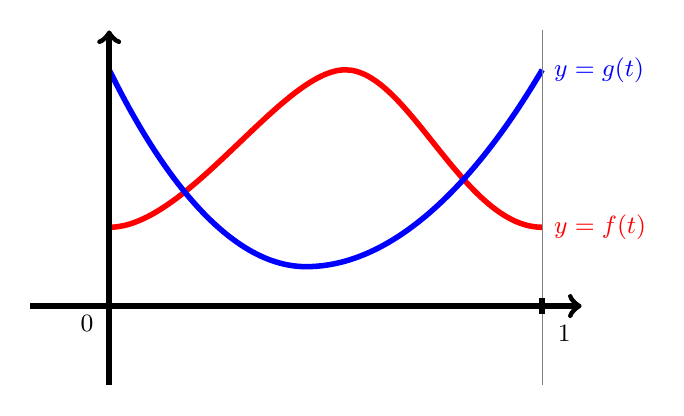
\begin{tikzpicture}
\draw[red, line width = 2pt] 
(0, 1) 
..controls +(1, 0) and +(-0.8, 0) ..
(3, 3)
..controls +(0.8, 0) and +(-1, 0) ..
(5.5, 1) node[right] {\small $y = f(t)$};

\draw[blue, line width = 2pt] (0, 3) parabola bend (2.5,0.5) (5.5,3) node[right] {\small $y = g(t)$};

\draw[help lines] (5.5, -1) -- (5.5, 3.5);
\draw[->, line width = 2pt] (-1,0) -- (6,0);
\draw[->, line width = 2pt] (0,-1) -- (0,3.5);
\draw[line width = 2pt] (5.5, 0.1) -- (5.5, -0.1) node[below, xshift = 8pt] {\small $1$}; 
\node[below, xshift = -8pt] at (0,0) {\small $0$};
\end{tikzpicture}


\vskip  20mm

{\bf Example. } Compute the length of the function 
$$f(t) = 1 + t^{2}$$ 
in $C[0, 1]$.  




\newpage

\begin{cbox}[Definition]
Let $V$ be a vector space with an inner product $\innprod{\ , \ }$, and let $W$ be a subspace of $V$. 
A vector $\vv\in V$ is \emph{orthogonal to $W$} if $\innprod{\vv, \ww} = 0$ for all $\ww\in W$.  
\end{cbox}

\vskip 2mm

\begin{cbox}[Definition]
Let $V$ be a vector space with an inner product $\innprod{\ , \ }$, and let $W$ be a subspace of $V$. 
The \emph{orthogonal projection of  a vector $\vv\in V$ onto $W$}  is a vector $\proj_{W}\vv$ such that 
\benu
\item[{\bf 1)}]  $\proj_{W}\vv \in W$ \\[-4mm]
\item[{\bf 2)}]  the vector $\zz = \vv - \proj_{W}\vv$ is orthogonal to $W$.
\eenu
\end{cbox}

\vskip 2mm

\begin{cbox}[Best Approximation Theorem]
If $V$ is a vector space with an inner product $\innprod{\ , \ }$,  $W$ is a subspace of $V$, and 
$\vv\in V$, then $ \proj_{W}\vv$ is the vector of $V$ which is the closest to $\vv$:
$$\dist(\vv, \proj_{W}\vv) \leq \dist(\vv, \ww)$$
for all $\ww \in W$.  
\end{cbox}

\vskip 2mm

\begin{cbox}[Theorem]
Let $V$ is a vector space with an inner product $\innprod{\ , \ }$, and let $W$ be a subspace of $V$. 
If $\BB = \{\ww_{1}, \dots, \ww_{k} \}$ is an orthogonal basis of $W$ (i.e. a basis such that 
$\innprod{\ww_{i}, \ww_{j}} = 0$  for all $i\neq j$) then for $\vv\in V$ we have:
$$
\proj_{W}\vv = 
\frac{ \innprod{\vv, \ww_{1}} } {\innprod{\ww_{1}, \ww_{1} } } \ww_{1} + 
{\dots} + \frac{ \innprod{\vv, \ww_{k}} } {\innprod{\ww_{k}, \ww_{k} } } \ww_{k} 
$$
\end{cbox}


\newpage

\underline{\bf Application:} Fourier approximations.

\vskip 5mm

{\bf Goal:} Let $f\colon [0, 1] \to \R$ be a continuous function. Find the best possible approximation of $f$ of the form 
 \begin{alignat*}{3}
 P(t) = & \phantom{+} \ a_{0} && \\
  & + a_{1}\sin(2\pi t) &\  + \ \ & b_{1}\cos(2\pi t) \\
  & + a_{2}\sin(2\pi 2t) &\  + \ \ & b_{2}\cos(2\pi 2t) \\
  & \dots \ \ \dots \ \ \dots \ \ & \dots\ \  & \dots \ \ \dots \ \ \dots \\
  & + a_{n}\sin(2\pi nt) &\  + \ \ & b_{n}\cos(2\pi nt) \\
 \end{alignat*}

\vskip -10mm

\btikz[xscale = 3]
\begin{scope}[domain=0:1, samples = 200]
\draw[color=red,  line width = 2pt]   plot (\x,{sin(6.28*\x r)});
\draw[->, line width = 2pt] (-0.2,0) -- (1.2,0);
\draw[->, line width = 2pt] (0, -1.5) -- (0, 1.5);
\draw[help lines]  (1, -1.5) -- (1, 1.5);
\node[anchor = north west] at (1, 0){\small $1$};
\node[anchor = north east] at (0, 0){\small $0$};
\node[anchor = north] at (0.5, -1.2) {\small $\sin(2\pi t)$};
\end{scope}

\begin{scope}[domain=0:1, samples = 200, xshift = 20mm]
\draw[color=red,  line width = 2pt]   plot (\x,{sin(2*6.28*\x r)});
\draw[->, line width = 2pt] (-0.2,0) -- (1.2,0);
\draw[->, line width = 2pt] (0, -1.5) -- (0, 1.5);
\draw[help lines]  (1, -1.5) -- (1, 1.5);
\node[anchor = north west] at (1, 0){\small $1$};
\node[anchor = north east] at (0, 0){\small $0$};
\node[anchor = north] at (0.5, -1.2) {\small $\sin(2\pi 2t)$};
\end{scope}

\begin{scope}[domain=0:1, samples = 400, xshift = 40mm]
\draw[color=red,  line width = 2pt]   plot (\x,{sin(3*6.28*\x r)});
\draw[->, line width = 2pt] (-0.2,0) -- (1.2,0);
\draw[->, line width = 2pt] (0, -1.5) -- (0, 1.5);
\draw[help lines]  (1, -1.5) -- (1, 1.5);
\node[anchor = north west] at (1, 0){\small $1$};
\node[anchor = north east] at (0, 0){\small $0$};
\node[anchor = north] at (0.5, -1.2) {\small $\sin(2\pi 3t)$};
\end{scope}
\etikz
\btikz[xscale = 3]
\begin{scope}[domain=0:1, samples = 200]
\draw[color=blue,  line width = 2pt]   plot (\x,{cos(6.28*\x r)});
\draw[->, line width = 2pt] (-0.2,0) -- (1.2,0);
\draw[->, line width = 2pt] (0, -1.5) -- (0, 1.5);
\draw[help lines]  (1, -1.5) -- (1, 1.5);
\node[anchor = north west] at (1, 0){\small $1$};
\node[anchor = north east] at (0, 0){\small $0$};
\node[anchor = north] at (0.5, -1.2) {\small $\cos(2\pi t)$};
\end{scope}

\begin{scope}[domain=0:1, samples = 200, xshift = 20mm]
\draw[color=blue,  line width = 2pt]   plot (\x,{cos(2*6.28*\x r)});
\draw[->, line width = 2pt] (-0.2,0) -- (1.2,0);
\draw[->, line width = 2pt] (0, -1.5) -- (0, 1.5);
\draw[help lines]  (1, -1.5) -- (1, 1.5);
\node[anchor = north west] at (1, 0){\small $1$};
\node[anchor = north east] at (0, 0){\small $0$};
\node[anchor = north] at (0.5, -1.2) {\small $\cos(2\pi 2t)$};
\end{scope}

\begin{scope}[domain=0:1, samples = 400, xshift = 40mm]
\draw[color=blue,  line width = 2pt]   plot (\x,{cos(3*6.28*\x r)});
\draw[->, line width = 2pt] (-0.2,0) -- (1.2,0);
\draw[->, line width = 2pt] (0, -1.5) -- (0, 1.5);
\draw[help lines]  (1, -1.5) -- (1, 1.5);
\node[anchor = north west] at (1, 0){\small $1$};
\node[anchor = north east] at (0, 0){\small $0$};
\node[anchor = north] at (0.5, -1.2) {\small $\cos(2\pi 3t)$};
\end{scope}
\etikz

\vfill
{\bf Note:} Let $W_{n}$ be a subspace of $C[0,1]$ given by:
$$W_{n} = \Span(1, \sin(2\pi t), \cos(2\pi t), \dots, \sin(2\pi nt), \cos(2\pi nt))$$
By the Best Approximation Theorem, the best approximation of $f$ is obtained 
if we take $P(t) = \proj_{W_{n}}f(t)$.

\newpage


\begin{cbox}[Theorem]
The set 
$$\{1, \sin(2\pi t), \cos(2\pi t), \dots, \sin(2\pi nt), \cos(2\pi nt)\}$$
is an orthogonal basis of $W_{n}$. 
\end{cbox}

\vskip 2mm

\begin{cbox}[Corollary]
If $f\in C[0, 1]$ then 
\begin{alignat*}{3}
\proj_{W_{n}}f(t) = & \phantom{+} \ a_{0} && \\
  & + a_{1}\sin(2\pi t) &\  + \ \ & b_{1}\cos(2\pi t) \\
  & + a_{2}\sin(2\pi 2t) &\  + \ \ & b_{2}\cos(2\pi 2t) \\
  & \dots \ \ \dots \ \ \dots \ \ & \dots\ \  & \dots \ \ \dots \ \ \dots \\
  & + a_{n}\sin(2\pi nt) &\  + \ \ & b_{n}\cos(2\pi nt) \\
\end{alignat*}

\vskip -5mm

where:

\ 

\vskip 2mm

$\displaystyle a_{0} = \frac{\innprod{f, 1}} {\innprod{1, 1}} = \int_{0}^{1} f(t) dt$

\ 

\vskip 2mm


and for $k>0$:

\ 

\vskip 2mm

$\displaystyle a_{k} = \frac{\innprod{f, \sin(2\pi kt)}} {\innprod{\sin(2\pi kt), \sin(2\pi kt)}} 
= 2 \int_{0}^{1} f(t)\cdot \sin(2\pi kt) dt$

\ 

\vskip 2mm

$\displaystyle b_{k} = \frac{\innprod{f, \cos(2\pi kt)}} {\innprod{\cos(2\pi kt), \cos(2\pi kt)}} 
= 2 \int_{0}^{1} f(t)\cdot \cos(2\pi kt) dt$

\end{cbox}


\newpage

{\bf Example.} Compute $\proj_{W_{n}} f(t)$ for the function $f(t) = t$. 


\newpage

\underline{\bf Application:} Polynomial approximations.

\vskip 5mm

{\bf Goal:} Let $f\colon [0, 1] \to \R$ be a continuous function.  Find the best possible approximation of $f$ given 
by a polynomial $P(t)$ of degree $\leq n$: 
$$P(t) = a_{0}+ a_{1}t + {\dots} + a_{n}t^{n}$$

\vskip 40mm

{\bf Note:} Let $\Poly_{n}$ be the subspace of $C[0,1]$ consisting of all polynomials 
of degree $\leq n$:
$$\Poly_{n} = \{ a_{0}+ a_{1}t + {\dots} + a_{n}t^{n} \ | \ a_{k} \in \R \}$$
By the Best Approximation Theorem, the best approximation of $f$ is obtained 
if we take $P(t) = \proj_{\Poly_{n}}f(t)$.

\newpage


\underline{\bf Gram-Schmidt process:}

\vskip 5mm

\btikz[scale = 1.1, 
          line1/.style ={line width = 2pt, red, text=black},
          line2/.style  ={red!30, line width = 16},
          line3/.style  = {red!30, line width =  30, ->, >={Triangle[length = 14pt, width = 42pt]}}
          ]



\draw[line1] (0,0) rectangle +(4.2,2.2) node[pos=0.5] {\small \begin{tabular}{c} 
a basis \\[1mm] 
$\{\vv_{1}, \dots, \vv_{k}\}$ \\[1mm]
of $W\subseteq V$ \\
\end{tabular}};

\draw[line1] (7.5,0) rectangle +(4.2,2.2) node[pos=0.5] {\small \begin{tabular}{c} 
an orthogonal basis \\[1mm] 
$\{\ww_{1}, \dots, \ww_{k}\}$ \\[1mm]
of $W$ \\
\end{tabular}};

\draw[line3, shorten >= 1pt, shorten <= 1pt, text=red] (4.2, 1.1) -- (7.5, 1.1) 
    node[pos = 0.45] {\small \emph{G-S process}};
\etikz


\vskip 15mm

\begin{cbox}[Theorem (Gram-Schmidt Process)]
Let $V$ be a vector space with an inner product $\innprod{\ , \ }$, and let $W$ be a subspace of  $V$. 
Let $\{\vv_{1}, \dots, \vv_{k}\}$  be a basis of $W$. Define vectors $\{\ww_{1}, \dots, \ww_{k}\}$ as follows:

\vskip 10mm

\benu
\item[] $\ww_{1} = \vv_{1}$ \\[2mm]

\item[]  $\displaystyle \ww_{2} =  \vv_{2} - \frac{\innprod{\ww_{1}, \vv_{2}}}{\innprod{\ww_{1}, \ww_{1}}} \ww_{1}$  \\[2mm]
\item[]  $\displaystyle \ww_{3} = \vv_{3} - \frac{\innprod{\ww_{1}, \vv_{3}}}{\innprod{\ww_{1}, \ww_{1}}} \ww_{1}
 - \frac{ \innprod{\ww_{2}, \vv_{3} } } {\innprod{\ww_{2}, \ww_{2} } } \ww_{2}$ \\[0mm]
  \item[]  $\cdots \ \ \ \cdots \ \ \ \cdots \ \ \ \cdots \ \ \  \cdots \ \ \ \cdots \ \ \ \cdots \ \ \ \cdots \ \ \ \cdots \ \ \ $\\[0mm]
  \item[]  $\displaystyle \ww_{k} = \vv_{k} - \frac{\innprod{\ww_{1}, \vv_{k}}}{\innprod{\ww_{1}, \ww_{1}}} \ww_{1}
 - \frac{ \innprod{\ww_{2}, \vv_{k} } } {\innprod{\ww_{2}, \ww_{2} } } \ww_{2}  
 - {\dots}
  - \frac{ \innprod{\ww_{k-1}, \vv_{k} } } {\innprod{\ww_{k-1}, \ww_{k-1} } } \ww_{k-1}$\\[2mm]
\eenu
Then the set $\{\ww_{1}, \dots, \ww_{k}\}$ is an orthogonal basis of $W$. 
\end{cbox}


\newpage

{\bf Example.} Find an orthogonal basis of the subspace $\Poly_{2}$ of the vector space $C[0, 1]$.  


\newpage

{\bf Example.} Compute  $\proj_{\Poly_{2}}f(t)$ for $f(t) = \sqrt{t}$.  

%---------------------------
%  Part
%---------------------------
\lecture{Eigenvalues and eigenvectors}

\underline{\bf Recall:}  An $n\times n$ matrix $A$ defines a linear transformation 
$$T_{A} \colon \R^{n} \to \R^{n}$$
given by $T_{A}(\vv) = A\vv$. 


\vskip 5mm

\underline{\bf Next goal:} Understand this linear transformation better. 


\vskip 15mm


{\bf Example.}

\vskip 5mm

$A =  
\bbm
2 & 0 \\
0 & 3 \\
\ebm
$


\vskip 30mm

\btikz[scale = 0.8]

\begin{scope}
\foreach \x in {-4,...,4}{
\draw[help lines, color = black!30] (\x, -4) -- (\x, 4);
}
\foreach \y in {-4,...,4}{
\draw[help lines, color = black!30] (-4, \y) -- (4, \y);
}
\draw[->, line width = 2pt] (-4,0) -- (4,0);
\draw[->, line width = 2pt] (0,-4) -- (0,4);
\begin{scope}
\clip(-4,-4) rectangle (4,4);
\foreach \x in {0.5, 1.0,...,6.0}{
\draw[line width = 0.1pt] (0,0) circle (\x);
}
\end{scope}
\end{scope}
\begin{scope}[xshift = 130mm]
\foreach \x in {-4,...,4}{
\draw[help lines, color = black!30] (\x, -4) -- (\x, 4);
}
\foreach \y in {-4,...,4}{
\draw[help lines, color = black!30] (-4, \y) -- (4, \y);
}
\draw[->, line width = 2pt] (-4,0) -- (4,0);
\draw[->, line width = 2pt] (0,-4) -- (0,4);
\begin{scope}
\clip(-4,-4) rectangle (4,4);
\pgfpathellipse{\pgfpointxy{0}{0}}{\pgfpointxy{1}{0}}{\pgfpointxy{0}{1.5}}
\pgfpathellipse{\pgfpointxy{0}{0}}{\pgfpointxy{2}{0}}{\pgfpointxy{0}{3}}
\pgfpathellipse{\pgfpointxy{0}{0}}{\pgfpointxy{3}{0}}{\pgfpointxy{0}{4.5}}
\pgfpathellipse{\pgfpointxy{0}{0}}{\pgfpointxy{4}{0}}{\pgfpointxy{0}{6}}
\pgfpathellipse{\pgfpointxy{0}{0}}{\pgfpointxy{5}{0}}{\pgfpointxy{0}{7.5}}
\pgfpathellipse{\pgfpointxy{0}{0}}{\pgfpointxy{6}{0}}{\pgfpointxy{0}{9}}
\pgfsetlinewidth{0.1pt}
\pgfusepath{draw}
\end{scope}
\end{scope}
\etikz



\newpage


{\bf Example.}

\vskip 5mm

$A =  
\bbm
2 & 1 \\
1 & 2 \\
\ebm
$


\vskip 60mm

\btikz[scale = 0.8]

\begin{scope}
\foreach \x in {-4,...,4}{
\draw[help lines, color = black!30] (\x, -4) -- (\x, 4);
}
\foreach \y in {-4,...,4}{
\draw[help lines, color = black!30] (-4, \y) -- (4, \y);
}
\draw[->, line width = 2pt] (-4,0) -- (4,0);
\draw[->, line width = 2pt] (0,-4) -- (0,4);
\begin{scope}
\clip(-4,-4) rectangle (4,4);
\foreach \x in {0.5, 1.0,...,6.0}{
\draw[line width = 0.1pt] (0,0) circle (\x);
}
\end{scope}
\end{scope}
\begin{scope}[xshift = 130mm]
\foreach \x in {-4,...,4}{
\draw[help lines, color = black!30] (\x, -4) -- (\x, 4);
}
\foreach \y in {-4,...,4}{
\draw[help lines, color = black!30] (-4, \y) -- (4, \y);
}
\draw[->, line width = 2pt] (-4,0) -- (4,0);
\draw[->, line width = 2pt] (0,-4) -- (0,4);
\begin{scope}
\clip(-4,-4) rectangle (4,4);
\pgfpathellipse{\pgfpointxy{0}{0}}{\pgfpointxy{3}{3}}{\pgfpointxy{1}{-1}}
\pgfpathellipse{\pgfpointxy{0}{0}}{\pgfpointxy{1.5}{1.5}}{\pgfpointxy{0.5}{-0.5}}
\pgfpathellipse{\pgfpointxy{0}{0}}{\pgfpointxy{4.5}{4.5}}{\pgfpointxy{1.5}{-1.5}}
\pgfpathellipse{\pgfpointxy{0}{0}}{\pgfpointxy{6}{6}}{\pgfpointxy{2}{-2}}
\pgfpathellipse{\pgfpointxy{0}{0}}{\pgfpointxy{7.5}{7.5}}{\pgfpointxy{2.5}{-2.5}}
\pgfpathellipse{\pgfpointxy{0}{0}}{\pgfpointxy{9}{9}}{\pgfpointxy{3}{-3}}
\pgfpathellipse{\pgfpointxy{0}{0}}{\pgfpointxy{10.5}{10.5}}{\pgfpointxy{3.5}{-3.5}}
\pgfpathellipse{\pgfpointxy{0}{0}}{\pgfpointxy{12}{12}}{\pgfpointxy{4}{-4}}
\pgfsetlinewidth{0.1pt}
\pgfusepath{draw}
\end{scope}
\end{scope}
\etikz


\newpage


\begin{cbox}[Definition]
Let $A$ be an $n\times n$ matrix. If $\vv\in \R^{n}$ is a non-zero vector and $\lambda$ is a scalar such that 
$$A\vv = \lambda \vv$$
then we say that 
\benu
\item[\textbullet] $\lambda$ is an \emph{eigenvalue} of $A$ \\[-4mm]
\item[\textbullet] $\vv$ is an \emph{eigenvector} of $A$ corresponding to $\lambda$. 
\eenu

\end{cbox}


\vskip 5mm



{\bf Example.}

\vskip 5mm

$A =  
\bbm
2 & 0 \\
0 & 3 \\
\ebm
$


\vskip 50mm


{\bf Example.}

\vskip 5mm

$A =  
\bbm
2 & 1 \\
1 & 2 \\
\ebm
$

\newpage

\underline{\bf Computation of eigenvalues}

\vskip 10mm


{\bf Recall:} $I_{n} = $ $n\times n$ identity matrix:

 $$
 I_{n} = 
 \bbm
 1 & 0 & {\dots} & 0 \\
  0 & 1 & {\dots} & 0 \\
  \vdots & \vdots & \ddots & \vdots \\
  0 & 0 & {\dots} & 1 \\
 \ebm
 $$




\vskip 70mm

\begin{cbox}[Propostiton]
If $A$ be an $n\times n$ matrix then  $\lambda\in \R$ is an eigenvalue of $A$ if and only if 
the matrix equation 
$$(A- \lambda I_{n})\xx = \zzero$$
has a non-trivial solution. 
\end{cbox}





\newpage

\begin{cbox}[Propostiton]
If $B$ is an $n\times n$ matrix then equation 
$$B\xx = \zzero$$ 
has a non-trivial solution if and only of the matrix $B$ is not invertible. 
\end{cbox}


\vskip 80mm


\begin{cbox}[Propostiton]
If $A$ be an $n\times n$ matrix then  $\lambda\in \R$ is an eigenvalue of $A$ if and only if 
$$\det(A- \lambda I_{n}) = 0$$
\end{cbox}


\newpage

{\bf Example.} Find all eigenvalues of the following matrix:

$$
A = 
\bbm
2 & 2 & 1 \\
1 & 3 & 1 \\
1 & 2 & 2 \\
\ebm
$$


\newpage

\begin{cbox}[Definition]
If $A$ is an $n\times n$ matrix then 
$$P(\lambda) = \det(A - \lambda I_{n})$$
is a polynomial of degree $n$. $P(\lambda)$ is called the \emph{characteristic polynomial} of the matrix
$A$. 
\end{cbox}


\vskip 10mm

\begin{cbox}[Upshot]
If $A$ is a square matrix then 
$$\text{eigenvalues of } A  = \text{roots of } P(\lambda)$$
\end{cbox}

\vskip 5mm

{\bf Example.} 

\vskip 3mm

$
A = 
\bbm
2 & 2 & 1 \\
1 & 3 & 1 \\
1 & 2 & 2 \\
\ebm
$

\vskip 40mm

\begin{cbox}[Corollary]
An $n\times n$ matrix can have at most $n$ distinct eigenvalues. 
\end{cbox}

\newpage


\underline{\bf Computation of eigenvectors}

\vskip 40mm

\begin{cbox}[Proposition]
If $\lambda$ is an eigenvalue of an $n\times n$ matrix $A$ then
$$
\left\{
\begin{matrix}
\text{eigenvectors of $A$} \\
\text{corresponding to $\lambda$}
\end{matrix}
\right\}
= 
\left\{
\begin{matrix}
\text{vectors in} \\
\Nul(A - \lambda I_{n})
\end{matrix}
\right\}
$$
\end{cbox}

\newpage

\ 

\vskip 20mm


\begin{cbox}[Corollary/Definition]
If $A$ is an $n\times n$ matrix and $\lambda$ is an eigenvalue of $A$ then the set of all 
eigenvectors corresponding to $\lambda$ is a subspace of $\R^{n}$. 

\vskip 3mm

This subspace is called the \emph{eigenspace} of $A$ corresponding to $\lambda$. 
\end{cbox}


\vskip 10mm

\begin{cbox}[Proposition]
If $\lambda$ is an eigenvalue of an $n\times n$ matrix $A$ then
$$
\left\{
\begin{matrix}
\text{eigenspace of $A$} \\
\text{corresponding to $\lambda$}
\end{matrix}
\right\}
= 
\Nul(A - \lambda I_{n})
$$
\end{cbox}


\newpage

{\bf Example.}  Consider the following matrix:

\vskip 2mm

$$
A = 
\bbm
2 & 2 & 1 \\
1 & 3 & 1 \\
1 & 2 & 2 \\
\ebm
$$

\vskip 2mm

Recall  that eigenvalues of $A$ are $\lambda_{1} = 1$ and $\lambda_{2} = 5$. Compute bases of eigenspaces 
of $A$ corresponding to these eigenvalues. 


\vskip 15mm

{\bf Solution.}

\vskip 5mm


\underline{$\lambda_{1} = 1$}




\newpage

\underline{$\lambda_{2} = 5$}



%---------------------------
%  Part
%---------------------------
\lecture{Matrix diagonalization}

\underline{\bf Recall:}

\vskip 5mm

{\bf 1)} Let $A$ be an $n\times n$ matrix. If $\vv\in \R^{n}$ is a non-zero vector and $\lambda$ is a scalar such that 
$$A\vv = \lambda \vv$$
then
\benu
\item[\textbullet] $\lambda$ is an eigenvalue of $A$ \\[-4mm]
\item[\textbullet] $\vv$ is an eigenvector of $A$ corresponding to $\lambda$. 
\eenu

\vskip 15mm

{\bf 2)} The characteristic polynomial of an $n\times n$ matrix $A$ is the polynomial given by the formula
$$P(\lambda) = \det(A - \lambda I_{n})$$
where $I_{n}$ is the $n\times n$ identity matrix. 

\vskip 15mm

{\bf 3)}  If $A$ is a square matrix then 
$$\text{eigenvalues of } A  = \text{roots of } P(\lambda)$$

\vskip 10mm

{\bf 4)} If $\lambda$ is an eigenvalue of an $n\times n$ matrix $A$ then
$$
\left\{
\begin{matrix}
\text{eigenvectors of $A$} \\
\text{corresponding to $\lambda$}
\end{matrix}
\right\}
= 
\left\{
\begin{matrix}
\text{vectors in} \\
\Nul(A - \lambda I_{n})
\end{matrix}
\right\}
$$



\newpage


\underline{\bf Motivating example:} Fibonacci numbers

$$1, \ 1,\ 2, \ 3, \ 5, \ 8, \ 13, \ 21, \ 34, \ 55, \ 89, \ 144, \ 233,\ 377, \ \dots$$


\newpage

{\bf Problem.} Find a formula for the $n$-th Fibonacci number $F_{n}$. 




\newpage

{\bf General Problem.}  If $A$ is a square matrix how to compute $A^{k}$ quickly?

\vskip 10mm

Easy case:

\begin{cbox}[Definition]
A square matrix $D$ is \emph{diagonal matrix} if all its entries outside the main diagonal are zeros:
$$
D = 
\bbm[c]
\lambda_{1} & 0 & \dots & 0 \\
0 & \lambda_{2}  & \dots & 0 \\
\vdots & \vdots & \ddots & 0 \\
0 & 0 & \dots & \lambda_{n} \\
\ebm
$$
\end{cbox}


\vskip 40mm


\begin{cbox}[Proposition]
If $D$ is a diagonal matrix as above  then 
$$
D^{k} = 
\bbm[c]
\lambda^{k}_{1} & 0 & \dots & 0 \\
0 & \lambda^{k}_{2}  & \dots & 0 \\
\vdots & \vdots & \ddots & 0 \\
0 & 0 & \dots & \lambda^{k}_{n} \\
\ebm
$$
\end{cbox}


\newpage

\begin{cbox}[Definition]
A square matrix $A$ is a \emph{diagonalizable } if A is of the form
$$
A = PDP^{-1}
$$
where $D$ is a diagonal matrix and $P$ is an invertible matrix. 
\end{cbox}


{\bf Example.}
\
\vskip 5mm 

$A = 
\bbm
1 & 0 & 1 \\
0 & 1 & 1 \\
1 & 1 & 0 \\
\ebm
$ is a diagonalizable matrix:

\vskip 5mm 

$$
A = 
\bbm
1 & 1 & -1\\
1 & 1 & 1 \\
1 & -2 & 0 \\ 
\ebm
\cdot
\bbm
2 & 0 & 0 \\
0 & -1 & 0 \\
0 & 0 & 1 \\
\ebm
\cdot
\bbm
1 & 1 & -1\\
1 & 1 & 1 \\
1 & -2 & 0 \\ 
\ebm^{-1}
$$

\vskip 20mm


\begin{cbox}[Proposition]
If  $A$ is a diagonalizable matrix, $A = PDP^{-1}$, then 
$$A^{k} = PD^{k}P^{-1}$$
\end{cbox}


\newpage



{\bf Example.} 
\
\vskip 5mm 

Let $A = 
\bbm
1 & 0 & 1 \\
0 & 1 & 1 \\
1 & 1 & 0 \\
\ebm$. Compute $A^{10}$.


\newpage

\begin{cbox}[Diagonalization Theorem]
{\bf 1) } An $n\times n$ matrix   $A$ is a diagonalizable if and only if it has $n$ linearly independent 
eigenvectors $\vv_{1}, \vv_{2}, \dots, \vv_{n}$. 

\vskip 3mm

{\bf 2) }  In such case $A = PDP^{-1}$ where :

\vskip 3mm

\begin{tikzpicture}
\node at (0,0) {$
P = \bbm \vv_{1} & \vv_{2} & \dots & \vv_{n} \\ \ebm
$};
\node at (0, -2) {$
D = 
\bbm[c]
\lambda_{1} & 0 & \dots & 0 \\
0 & \lambda_{2}  & \dots & 0 \\
\vdots & \vdots & \ddots & 0 \\
0 & 0 & \dots & \lambda_{n} \\
\ebm
$};
\node at (8, -2){
\begin{tabular}{l}
$\lambda_{1}$ = eigenvalue corresponding to $\vv_{1}$ \\
$\lambda_{2}$ = eigenvalue corresponding to $\vv_{2}$ \\
$\dots \ \ \ \dots \ \ \ \dots \ \ \ \dots \ \ \ \dots \ \ \ \dots \ \ \ \dots$ \\
$\lambda_{n}$ = eigenvalue corresponding to $\vv_{n}$ \\
\end{tabular}
};
\end{tikzpicture}
\end{cbox}

\newpage

{\bf Example.} Diagonalize the following matrix if possible:

$$A = 
\bbm
4 & 0 & 0 \\
1 & 3 & -1 \\
1 & -1 & 3 \\
\ebm
$$


\newpage 

{\bf Note.} Not every matrix is diagonalizable.

\vskip 5mm

{\bf Example.} Check if the following matrix is diagonalizable:

$$A = 
\bbm
2 & 1 \\
0 & 2 \\
\ebm
$$

\newpage

\begin{cbox}[Proposition]
If $A$ is an $n\times n$ matrix with $n$ distinct eigenvalues then $A$ is diagonalizable. 
\end{cbox}


\newpage

\underline{\bf Back to Fibonacci numbers:}

\vskip 3mm

$$
\bbm[l]
F_{n} \\ 
F_{n+1} \\
\ebm
= 
\bbm
0 & 1 \\
1 & 1 \\
\ebm^{n-1}
\cdot
\bbm
1 \\
1 \\
\ebm
$$


%---------------------------
%  Part
%---------------------------
\lecture{Diagonalization of symmetric matrices}


\underline{\bf Recall:}

\vskip 5mm

{\bf 1)} A square matrix $A$ is diagonalizable if there exists an invertible matrix $P$ and a diagonal matrix
$D$ such that 
$$A = PDP^{-1}$$

\vskip 15mm

{\bf 2)}  If $A$ is diagonalizable then it is easy to compute powers of $A$:
$$A^{k} = PD^{k}P^{-1}$$

\vskip 15mm

{\bf 3)} An $n\times n$ matrix   $A$ is a diagonalizable if and only if it has $n$ linearly independent 
eigenvectors $\vv_{1}, \vv_{2}, \dots, \vv_{n}$.  In such case  we have:

\vskip 10mm

\begin{tikzpicture}
\node at (0,0) {$
P = \bbm[c] \vv_{1} & \vv_{2} & \dots & \vv_{n} \\ \ebm
$};
\node at (0, -2) {$
D = 
\bbm[c]
\lambda_{1} & 0 & \dots & 0 \\
0 & \lambda_{2}  & \dots & 0 \\
\vdots & \vdots & \ddots & 0 \\
0 & 0 & \dots & \lambda_{n} \\
\ebm
$};
\node at (8, -2){
\begin{tabular}{l}
$\lambda_{1}$ = eigenvalue corresponding to $\vv_{1}$ \\
$\lambda_{2}$ = eigenvalue corresponding to $\vv_{2}$ \\
$\dots \ \ \ \dots \ \ \ \dots \ \ \ \dots \ \ \ \dots \ \ \ \dots \ \ \ \dots$ \\
$\lambda_{n}$ = eigenvalue corresponding to $\vv_{n}$ \\
\end{tabular}
};
\end{tikzpicture}


\vskip 15mm

{\bf 4)}  Not every square matrix is diagonalizable. 




\newpage

\begin{cbox}[Definition]
A square matrix  $A$  is \emph{symmetric} if $A^{T} = A$ 
\end{cbox}


\vskip 20mm

$$
\bbm
1 & 2 & 3 & 4 \\
2 & 0 & 5 & 6 \\
3 & 5 & 7 & 8 \\
4 & 6 & 8 & 9 \\
\ebm
$$


\vskip 60mm

\begin{cbox}[Theorem]
Every symmetric matrix is diagonalizable. 
\end{cbox}


\newpage

\begin{cbox}[Theorem]
If $A$ is a symmetric matrix and $\lambda_{1}, \lambda_{2}$ are two different eigenvalues of $A$, 
then eigenvectors corresponding to $\lambda_{1}$ are orthogonal to eigenvectors corresponding to 
$\lambda_{2}$. 
\end{cbox}

\vskip 5mm

{\bf Note.} If $\vv$, $\ww$ are vectors in $\R^{n}$ then 
$$\vv \cdot \ww = \vv^{T}\ww$$



\vskip 5mm

{\bf Example.}

\vskip 5mm

$\vv = \bbm 1 \\ 2 \\ 3 \\\ebm$, $\ww = \bbm 4 \\ 5 \\ 6 \\\ebm$


\newpage

\begin{cbox}[Theorem]
If $A$ is an $n\times n$ symmetric matrix then $A$ has $n$ orthogonal eigenvectors. 
\end{cbox}

\vskip 5mm

{\bf Example.}

{\bf a)} Find three orthogonal eigenvectors of the following symmetric matrix:
$$
A = 
\bbm
2 & 1 & 1 \\
1 & 2 & 1 \\
1 & 1 & 2 \\
\ebm
$$
{\bf b)} Use these eigenvectors to diagonalize this matrix. 


\newpage

\phantom{filler} 


\vfill 
\underline{\bf Upshot.} How to find $n$ orthogonal eigenvectors for a symmetric $n\times n$ matrix $A$:

\vskip 5mm

\benu[leftmargin=*]
\item[\bf 1)] Find eigenvalues of $A$. \\[-4mm]
\item[\bf 2)]  Find a basis of the eigenspace for each eigenvalue.  \\[-4mm]
\item[\bf 3)]  Use the Gram-Schmidt process to find an orthogonal basis of each eigenspace. 
\eenu


\newpage


\ 

\vfill

\begin{cbox}[Definition]
A square matrix $Q = \bbm \uu_{1} & \uu_{2} & \dots & \uu_{n} \\ \ebm$ is an \emph{orthogonal matrix}
if $\{\uu_{1}, \uu_{2}, \dots, \uu_{n}\}$ is an orthonormal set of vectors, i.e.:
$$
\uu_{i}\cdot \uu_{j} = 
\begin{cases}
1 & \text{if $i= j$} \\
0 & \text{if $i\neq j$} \\
\end{cases}
$$ 
\end{cbox}


\vskip 10mm

\begin{cbox}[Theorem]
If $Q$ is an orthogonal matrix then $Q$ is invertible and  $Q^{-1} = Q^{T}$.
\end{cbox}

\newpage



{\bf Note.} If $P = \bbm \vv_{1} & \vv_{2} & \dots & \vv_{n} \\ \ebm$ is a matrix with orthogonal columns, 
then 
$$
Q = 
\bbm
\displaystyle{\frac{\vv_{1}}{\norm{\vv_{1}}}}  & 
\displaystyle{\frac{\vv_{2}}{\norm{\vv_{2}}}}  & 
{\dots} & 
\displaystyle{\frac{\vv_{n}}{\norm{\vv_{n}}}} \\
\ebm
$$
is an orthogonal matrix. 


\vskip 20mm

\begin{cbox}[Theorem]
If $A$ is a symmetric matrix then $A$ is \emph{orthogonally diagonalizable}. That is, there exists 
an orthogonal matrix $Q$ and a diagonal matrix $D$ such that 
$$A = QDQ^{-1} = QDQ^{T}$$
\end{cbox}


\newpage

{\bf Example.} Find an orthogonal diagonalization of the following symmetric matrix:
$$
A = 
\bbm
2 & 1 & 1 \\
1 & 2 & 1 \\
1 & 1 & 2 \\
\ebm
$$




\newpage

{\bf Note. } We have seen that any symmetric matrix is orthogonally diagonalizable. The converse statement 
is also true:

\begin{cbox}[Proposition]
If a matrix $A$ is orthogonally diagonalizable then $A$ is a symmetric matrix. 
\end{cbox}



%---------------------------
%  Part
%---------------------------
\lecture{Spectral decomposition of symmetric matrices}


\underline{\bf Recall:}

\vskip 5mm

{\bf 1)} An orthogonal matrix $Q = \bbm \uu_{1} & \uu_{2} & \dots & \uu_{n} \\ \ebm$ is a square matrix  such that
 $\{\uu_{1}, \uu_{2}, \dots, \uu_{n}\}$ is an orthonormal set of vectors, i.e.:
$$
\uu_{i}\cdot \uu_{j} = 
\begin{cases}
1 & \text{if $i= j$} \\
0 & \text{if $i\neq j$} \\
\end{cases}
$$ 

\vskip 15mm

{\bf 2)} If $Q$ is an orthogonal matrix then $Q^{-1} = Q^{T}$

\vskip 15mm

{\bf 3)}  A square matrix $A$ is orthogonally diagonalizable  if there exist
an orthogonal matrix $Q$ and a diagonal matrix $D$ such that 
$$A = QDQ^{-1} = QDQ^{T}$$

\vskip 15mm

{\bf 4)} A matrix $A$ is orthogonally diagonalizable if and only if $A$ is a symmetric matrix (i.e. $A^{T} = A$). 





\newpage



\underline{\bf Yet another view of matrix multiplication}

\vskip 5mm

{\bf Note.} If $C$ is an $n\times 1$ matrix and $D$ is an $1\times n$ matrix then $CD$ is an $n\times n$
matrix. 

\vskip 40mm

\begin{cbox}[Propostion]
Let $A$ be an $n\times n$ matrix with columns $\vv_{1}, \dots, \vv_{n}$, and $B$ be an $n\times n$ matrix 
with rows $\ww_{1}, \dots, \ww_{n}$:
$$A = 
\bbm
\vv_{1} & \dots & \vv_{n} \\
\ebm
\hskip 10mm
B = \begin{bmatrix} \ww_{1} \\ \vdots \\ \ww_{n} \\ \end{bmatrix}
$$
Then 
$$AB = \vv_{1}\ww_{1} + \vv_{2}\ww_{2} + {\dots} + \vv_{n}\ww_{n}$$
\end{cbox}

\vskip 5mm

{\bf Example.}

\vskip 5mm

$A = \bbm 1 & 2 \\ 3 & 4 \\ \ebm$ \hskip 10mm $B = \bbm 5 & 1 \\ 7 & 2 \\ \ebm$

\newpage


\begin{cbox}[Theorem]
Let $A$ be a symmetric matrix with orthogonal diagonalization
$$A = QDQ^{T}$$
If 
$$
Q = 
\bbm \uu_{1} & \dots & \uu_{n} \\ \ebm
\ \ \ \text{and} \ \ \ 
D = 
\bbm[c]
\lambda_{1}  & \dots & 0 \\
\vdots & \ddots & 0 \\
0 &  \dots & \lambda_{n} \\
\ebm
$$
then  
$$A = \lambda_{1}(\uu_{1}\uu_{1}^{T}) + \lambda_{2}(\uu_{2}\uu_{2}^{T}) + {\dots} + \lambda_{n}(\uu_{n}\uu_{n}^{T})$$ 
\end{cbox}


{\bf Note.} The above formula is called the \emph{spectral decomposition} of the matrix $A$. 


\newpage

{\bf Example.}

\vskip 5mm

$$
\bbm
3 &  1  \\ 
1 &  3 \\ 
\ebm = 
\bbm
1/\sqrt{2} &  -1/\sqrt{2}  \\ 
1/\sqrt{2} &  1/\sqrt{2} \\ 
\ebm
\cdot
\bbm
4 &  0  \\ 
0 &  2 \\ 
\ebm
\cdot
\bbm
1/\sqrt{2} &   -1/\sqrt{2}  \\ 
1/\sqrt{2} &  1/\sqrt{2} \\ 
\ebm^{T} 
$$

\newpage

\begin{center}
\underline{\bf Spectral decomposition and linear transformations}
\end{center}

$$
\bbm
3 &  1  \\ 
1 &  3 \\ 
\ebm = 
\bbm
1/\sqrt{2} &  -1/\sqrt{2}  \\ 
1/\sqrt{2} &  1/\sqrt{2} \\ 
\ebm
\cdot
\bbm
4 &  0  \\ 
0 &  2 \\ 
\ebm
\cdot
\bbm
1/\sqrt{2} &   -1/\sqrt{2}  \\ 
1/\sqrt{2} &  1/\sqrt{2} \\ 
\ebm^{T} 
$$

\vskip 15mm

\begin{flushright}
\begin{tikzpicture}[scale = 0.9]
\draw[->, line width = 2pt] (-5,0) -- (5,0);
\draw[->, line width = 2pt] (0,-5) -- (0,5);
\end{tikzpicture}
\end{flushright}





%---------------------------
%  Part
%---------------------------
\lecture{Application: Symmetric image compression}


\begin{tikzpicture}
\node[anchor = north west, inner sep=0,outer sep=0] at (0, 0) {
\includegraphics[width=85mm]{symm_einstein.jpg}
};
\node[anchor = north west] at (8.5, 0){
\begin{minipage}{85mm}
\benu
\item[\textbullet] The size of this image is 1000$\times$ 1000 pixels. \\[-2.5mm]

\item[\textbullet] The color of each pixel is represented by an integer 
between 0 (black) and 255 (white). \\[-2.5mm]

\item[\textbullet] The whole image is described by a (symmetric) matrix $A$ 
consisting of $1000\times 1000 = 1,000,000$ numbers   \\[-2.5mm]

\item[\textbullet]  Each number is stored in 1 byte, so the image file size is 
$1,000,000$ bytes ($\approx 1$ MB). 
\eenu
\end{minipage}
};
\end{tikzpicture}


\vskip  20mm

{\bf How to make the image file smaller:}

\vskip 5mm

{\bf 1)} Find the spectral decomposition of the matrix $A$:
$$A = \lambda_{1}(\uu_{1}\uu_{1}^{T}) + \lambda_{2}(\uu_{2}\uu_{2}^{T}) + {\dots} + \lambda_{1000}(\uu_{1000}\uu_{1000}^{T})$$ 
where $|\lambda_{1}| \geq |\lambda_{2}| \geq {\dots} \geq |\lambda_{1000}|$.

\vskip 20mm

{\bf 2)} For $k = 1, \dots, 1000$ define:
$$B_{k} = \lambda_{1}(\uu_{1}\uu_{1}^{T}) + \lambda_{2}(\uu_{2}\uu_{2}^{T}) + {\dots} + \lambda_{k}(\uu_{k}\uu_{k}^{T})$$ 
This matrix approximates the matrix $A$ and can be stored using $k\cdot(1000 + 1)$ numbers 
(i.e. $k\cdot(1000 + 1)$ bytes).  


\newpage

\begin{center}
{\bf Eigenvalues of the matrix $\mathbf A$}
\vskip 5mm

\includegraphics[width=0.9\textwidth]{einstein_eigenvalues.pdf}
\end{center}

\vskip 20mm

\begin{tikzpicture}
\node[anchor = north west, inner sep=0,outer sep=0] at (0, 0) {
\includegraphics[width=83mm]{symm_einstein1.jpg}
};
\node[anchor = north west,  inner sep=0,outer sep=0] at (0, -8.5){
\small
\begin{tabular}{l}
{\bf matrix $\mathbf B_{1}$} \\
1001 bytes \\
compression 1000:1
\end{tabular}
};
\node[anchor = north west, , inner sep=0,outer sep=0] at (9, 0){
\includegraphics[width=83mm]{symm_einstein5.jpg}
};
\node[anchor = north west,  inner sep=0,outer sep=0] at (9, -8.5){
\small
\begin{tabular}{l}
{\bf matrix $\mathbf B_{5}$} \\
5005 bytes \\
compression 200:1
\end{tabular}
};
\end{tikzpicture}





\newpage

\begin{tikzpicture}
\node[anchor = north west, inner sep=0,outer sep=0] at (0, 0) {
\includegraphics[width=83mm]{symm_einstein10.jpg}
};
\node[anchor = north west,  inner sep=0,outer sep=0] at (0, -8.5){
\small
\begin{tabular}{l}
{\bf matrix $\mathbf B_{10}$} \\
10,010 bytes \\
compression 100:1
\end{tabular}
};
\node[anchor = north west, , inner sep=0,outer sep=0] at (9, 0){
\includegraphics[width=83mm]{symm_einstein20.jpg}
};
\node[anchor = north west,  inner sep=0,outer sep=0] at (9, -8.5){
\small
\begin{tabular}{l}
{\bf matrix $\mathbf B_{20}$} \\
20,020 bytes \\
compression 50:1
\end{tabular}
};
\end{tikzpicture}


\vskip 10mm

\begin{tikzpicture}
\node[anchor = north west, inner sep=0,outer sep=0] at (0, 0) {
\includegraphics[width=83mm]{symm_einstein50.jpg}
};
\node[anchor = north west,  inner sep=0,outer sep=0] at (0, -8.5){
\small
\begin{tabular}{l}
{\bf matrix $\mathbf B_{50}$} \\
50,050 bytes \\
compression 20:1
\end{tabular}
};
\node[anchor = north west, , inner sep=0,outer sep=0] at (9, 0){
\includegraphics[width=83mm]{symm_einstein100.jpg}
};
\node[anchor = north west,  inner sep=0,outer sep=0] at (9, -8.5){
\small
\begin{tabular}{l}
{\bf matrix $\mathbf B_{100}$} \\
100,100 bytes \\
compression 10:1
\end{tabular}
};
\end{tikzpicture}



%---------------------------
%  Part
%---------------------------
\lecture{Singular Value Decomposition}

\vskip -3mm

\begin{cbox}[Theorem]
Any $A$ an $m\times n$ matrix can be written as a product
$$A = U\Sigma V^{T}$$

\vskip -4mm

where:
\benu
\item[\textbullet] $U = \bbm[c] \uu_{1} & \dots & \uu_{m} \\ \ebm$ is an $m\times m$ orthogonal matrix.\\[-3mm]
\item[\textbullet] $V = \bbm[c] \vv_{1} & \dots & \vv_{n} \\ \ebm$ is an $n\times n$ orthogonal matrix. \\[-3mm]
\item[\textbullet] $\Sigma$ is an $m\times n$ matrix of the following form: 
\btikz
\node at (0, 0){\small $
\bbm[c]
\sigma_{1} & 0 & \cdots & 0 \\
0 & \sigma_{2}  & \cdots & 0 \\
\vdots & \vdots & \ddots & 0 \\
0 & 0 & \cdots & \sigma_{n} \\
0 & 0 & \cdots & 0 \\
\cdots & \cdots & \cdots & \cdots \\
0 & 0 & \cdots & 0 \\
\ebm
$};

\node at (8, 0){\small $
\bbm[c]
\sigma_{1} & 0 & \cdots & 0  & 0 & \cdots & 0\\
0 & \sigma_{2}  & \cdots & 0 & 0 & \cdots & 0\\
\vdots & \vdots & \ddots & 0 & 0 & \cdots & 0\\
0 & 0 & \cdots & \sigma_{m} & 0 & \cdots & 0\\
\ebm
$};

\node at (3.3, 0) {or};
\node at (0 , -2.8) {(if $n\leq m$)}; 
\node at (8 , -2.8) {(if $n \geq m$)};
\etikz
where $\sigma_{1} \geq \sigma_{2} \geq {\dots} \geq 0$.   
\eenu
\end{cbox}


{\bf Note.} 
\benu[leftmargin = *]
\item[\textbullet] The numbers $\sigma_{1}, \sigma_{2}, \dots$ are called \emph{singular values} of $A$. \\[-3mm]

\item[\textbullet]  The vectors $\uu_{1}, \dots, \uu_{m}$ are called  
\emph{left singular vectors} of $A$. \\[-3mm]

\item[\textbullet]  Then the vectors $\vv_{1}, \dots, \vv_{n}$ are called  
\emph{right singular vectors} of $A$. \\[-3mm]

\item[\textbullet] {\SetTracking{encoding=*}{-10}\lsstyle
The formula $A = U\Sigma V^{T}$ is called a \emph{singular value decomposition (SVD)} of $A$.} \\[-3mm]

\item[\textbullet] The matrix $\Sigma$ is uniquely determined, but $U$ and $V$ depend on some choices. 
\eenu


\newpage


\begin{cbox}[Theorem]
Let $A$ be a matrix with a singular value decomposition
$$A = U\Sigma V^{T}$$
If 
$$
U = 
\bbm[c] \uu_{1} & \dots & \uu_{m} \\ \ebm
\hskip 10mm
V = 
\bbm[c] \vv_{1} & \dots & \vv_{n} \\ \ebm
$$
and $\sigma_{1}, \dots, \sigma_{r}$ are singular values of $A$ then
then  
$$A = \sigma_{1}(\uu_{1}\vv_{1}^{T}) + \sigma_{2}(\uu_{2}\vv_{2}^{T}) + {\dots} + \sigma_{r}(\uu_{r}\vv_{r}^{T})$$ 
\end{cbox}

\newpage

\underline{\bf Application:} {\bf Image compression}

\vskip 10mm

\begin{tikzpicture}
\node[anchor = north west, inner sep=0,outer sep=0] at (0, 0) {
\includegraphics[width=75mm]{mcurie.jpg}
};
\node[anchor = north west] at (7.5, 0){
\begin{minipage}{95mm}
\benu
\item[\textbullet] The size of this image is 800$\times$700 pixels. \\[-2.5mm]

\item[\textbullet] The color of each pixel is represented by an integer 
between 0 (black) and 255 (white). \\[-2.5mm]

\item[\textbullet] The whole image is described by a matrix $A$ 
consisting of $800 \times 700$ $ = 560,000$ numbers.   \\[-2.5mm]

\item[\textbullet]  Each number is stored in 1 byte, so the image file size is 
$560,000$ bytes ($\approx 0.53$ MB). 
\eenu
\end{minipage}
};
\end{tikzpicture}

\vskip 3mm

{\bf How to make the image file smaller:}

\vskip 5mm

{\bf 1)} Compute SVD of the matrix $A$:
$$A = U\Sigma V^{T}$$
where
$$
U = 
\bbm[c] \uu_{1} & \dots & \uu_{m} \\ \ebm
\hskip 10mm
V = 
\bbm[c] \vv_{1} & \dots & \vv_{n} \\ \ebm
$$
and $\sigma_{1}, \dots, \sigma_{r}$ are singular values of $A$. 

\vskip 8mm

{\bf 2)} Replace $A$ by the matrix  
$$B_{k} = \sigma_{1}(\uu_{1}\vv_{1}^{T}) + {\dots} + \sigma_{k}(\uu_{k}\vv_{k}^{T})$$ 
for some $1\leq k \leq 700$. This matrix can be stored using $k\cdot (800  + 700  + 1)$ numbers. 



\newpage

\begin{center}
{\bf Singular values of the matrix $\mathbf A$}
\vskip 5mm

\includegraphics[width=0.9\textwidth]{mcurie_eigenvalues.pdf}
\end{center}

\vskip 20mm

\begin{tikzpicture}
\node[anchor = north west, inner sep=0,outer sep=0] at (0, 0) {
\includegraphics[width=75mm]{mcurie1.jpg}
};
\node[anchor = north west,  inner sep=0,outer sep=0] at (0, -9){
\small
\begin{tabular}{l}
{\bf matrix $\mathbf B_{1}$} \\
1501 bytes \\
compression 374:1
\end{tabular}
};
\node[anchor = north west, , inner sep=0,outer sep=0] at (9, 0){
\includegraphics[width=75mm]{mcurie5.jpg}
};
\node[anchor = north west,  inner sep=0,outer sep=0] at (9, -9){
\small
\begin{tabular}{l}
{\bf matrix $\mathbf B_{5}$} \\
7905 bytes \\
compression 75:1
\end{tabular}
};
\end{tikzpicture}





\newpage

\begin{tikzpicture}
\node[anchor = north west, inner sep=0,outer sep=0] at (0, 0) {
\includegraphics[width=75mm]{mcurie10.jpg}
};
\node[anchor = north west,  inner sep=0,outer sep=0] at (0, -9){
\small
\begin{tabular}{l}
{\bf matrix $\mathbf B_{10}$} \\
15,010 bytes \\
compression 37:1
\end{tabular}
};
\node[anchor = north west, , inner sep=0,outer sep=0] at (9, 0){
\includegraphics[width=75mm]{mcurie20.jpg}
};
\node[anchor = north west,  inner sep=0,outer sep=0] at (9, -9){
\small
\begin{tabular}{l}
{\bf matrix $\mathbf B_{20}$} \\
30,020 bytes \\
compression 18:1
\end{tabular}
};
\end{tikzpicture}

\vskip 10mm

\begin{tikzpicture}
\node[anchor = north west, inner sep=0,outer sep=0] at (0, 0) {
\includegraphics[width=75mm]{mcurie50.jpg}
};
\node[anchor = north west,  inner sep=0,outer sep=0] at (0, -9){
\small
\begin{tabular}{l}
{\bf matrix $\mathbf B_{50}$} \\
75,050 bytes \\
compression 7:1
\end{tabular}
};
\node[anchor = north west, , inner sep=0,outer sep=0] at (9, 0){
\includegraphics[width=75mm]{mcurie100.jpg}
};
\node[anchor = north west,  inner sep=0,outer sep=0] at (9, -9){
\small
\begin{tabular}{l}
{\bf matrix $\mathbf B_{100}$} \\
150,100 bytes \\
compression 4:1
\end{tabular}
};
\end{tikzpicture}






\newpage



\begin{center}
\underline{\bf How to compute SVD of a matrix $A$}
\end{center}


\newpage

\begin{center}
\underline{\bf How to compute SVD of a matrix $A$}
\end{center}

\vskip 5mm

\benu[leftmargin = *]
\item[{\bf 1)}] Compute an orthogonal diagonalization of the symmetric $n\times n$ matrix $A^{T}A$:
$$A^{T}A = QDQ^{T}$$
such that  eigenvalues on the diagonal of the matrix $D$ are arranged from the largest to the smallest. 
We set $V = Q$. \\[10mm]
\item[{\bf 2)}]  If 
$$
D = 
\bbm[c]
\lambda_{1} & 0 & \dots & 0 \\
0 & \lambda_{2}  & \dots & 0 \\
\vdots & \vdots & \ddots & 0 \\
0 & 0 & \dots & \lambda_{n} \\
\ebm
$$
then $\sigma_{i} = \sqrt{\lambda_{i}}$. This gives the matrix $\Sigma$. 

\ 

Note: if $n >  m$ then we use only $\lambda_{1}, \dots, \lambda_{m}$. The remaining eigenvalues 
$\lambda_{m+1}, \dots, \lambda_{n}$ of $D$ will be equal to $0$ in this case.  \\[10mm]

\item[{\bf 3)}] Let $V = \bbm[c] \vv_{1} & \dots & \vv_{n} \\ \ebm$,
 and let $\sigma_{1}, \dots, \sigma_{r}$ be non-zero singular values of $A$. 
The first $r$ columns of the matrix $U = \bbm[c] \uu_{1} & \dots & \uu_{m} \\ \ebm $ are given by 
$$\uu_{i} = \frac{1}{\sigma_{i}} A\vv_{i}$$


The remaining columns $\uu_{r+1}, \dots, \uu_{m}$ can be added arbitrarily so that 
$U$ is an orthogonal matrix (i.e.$ \{\uu_{1}, \dots, \uu_{m} \}$) is an orthonormal basis of $\R^{m}$. 

\eenu

\newpage

{\bf Example.} Find SVD of the following matrix: 
%\color{red} Strang p.444, Example 4
$$A = 
\bbm
-1 & 0 \\
1 & -1 \\
0 &  1 \\
\ebm
$$


\newpage


%---------------------------
%  Part
%---------------------------
\lecture{Application:  SVD and data analysis}


\underline{\bf Recall:}

Let $A$ be a matrix with a singular value decomposition 
$$A = U\Sigma V^{T}$$
If 
$$
U = 
\bbm[c] \uu_{1} & \dots & \uu_{m} \\ \ebm
\hskip 10mm
V = 
\bbm[c] \vv_{1} & \dots & \vv_{n} \\ \ebm
$$
and $\sigma_{1}, \dots, \sigma_{r}$ are singular values of $A$ then
then  
$$A = \sigma_{1}(\uu_{1}\vv_{1}^{T}) + \sigma_{2}(\uu_{2}\vv_{2}^{T}) + {\dots} + \sigma_{r}(\uu_{r}\vv_{r}^{T})$$ 



\vskip 15mm


{\bf Example:} Movie ratings:


\btikz[
          table/.style = {
          matrix of nodes,
          nodes={text width=1.25ex,align=center},
          nodes in empty cells
          },
          colh/.style = {
          rotate= 60,
          anchor = west,
          font=\bfseries,
          },
          rowh/.style = {
          anchor = east,
          font=\bfseries,
          xshift = -2mm,
          },
         ]
          


\matrix[table] (mat) 
{
5 & 0 & 5 & 0 & 4 \\
5 & 0 & 3 & 0 & 5 \\
0 & 5 & 0 & 5 & 1 \\
1 & 5 & 0 & 4 & 0 \\
4 & 0 & 4 & 0 & 3 \\
0 & 5 & 0 & 4 & 0 \\
3 & 0 & 3 & 0 & 2 \\
};

\node[colh]  at  ([yshift = 1ex] mat-1-1.north) {\small Matrix};
\node[colh]  at  ([yshift = 1ex] mat-1-2.north) {\small Amelie};
\node[colh]  at  ([yshift = 1ex] mat-1-3.north) {\small Alien};
\node[colh]  at  ([yshift = 1ex] mat-1-4.north) {\small Casablanca};
\node[colh]  at  ([yshift = 1ex] mat-1-5.north) {\small Interstellar};

\node[rowh]  at  (mat-1-1.west) {user\_1};
\node[rowh]  at  (mat-2-1.west) {user\_2};
\node[rowh]  at  (mat-3-1.west) {user\_3};
\node[rowh]  at  (mat-4-1.west) {user\_4};
\node[rowh]  at  (mat-5-1.west) {user\_5};
\node[rowh]  at  (mat-6-1.west) {user\_6};
\node[rowh]  at  (mat-7-1.west) {user\_7};
\etikz


\newpage

Singular value decomposition of the matrix of movie ratings:

\vskip 10mm

{\footnotesize
$
U = 
\begin{bmatrix*}[r]
-0.6 & 0.1 & -0.3 & -0.2 & 0.2 & -0.7 & -0.2 \\
-0.5 & 0.1 & 0.8 & 0.2 & 0.1 & 0.1 & 0.1 \\
-0.1 & -0.6 & 0.2 & -0.7 & -0.4 & 0.0 & 0.0 \\
-0.1 & -0.5 & -0.1 & 0.7 & -0.4 & -0.1 & -0.2 \\
-0.5 & 0.1 & -0.3 & -0.1 & -0.1 & 0.7 & -0.4 \\
-0.1 & -0.6 & -0.1 & 0.0 & 0.8 & 0.1 & 0.2 \\
-0.3 & 0.1 & -0.3 & 0.0 & -0.3 & 0.1 & 0.8 \\
\end{bmatrix*}
\hskip 2mm
\Sigma = 
\bbm
13.6 & 0 & 0 & 0 & 0 \\
0 & 11.4 & 0 & 0 & 0 \\
0 & 0 & 1.9 & 0 & 0 \\
0 & 0 & 0 & 1.1 & 0 \\
0 & 0 & 0 & 0 & 0.3 \\
0 & 0 & 0 & 0 & 0 \\
0 & 0 & 0 & 0 & 0 \\
\ebm
$

\vskip 6mm

$
V = 
\begin{bmatrix*}[r]
-0.6 & 0.1 & 0.0 & 0.7 & -0.4 \\
-0.1 & -0.7 & -0.1 & 0.3 & 0.6 \\
-0.5 & 0.1 & -0.7 & -0.4 & 0.2 \\
-0.1 & -0.6 & 0.0 & -0.4 & -0.7 \\
-0.5 & 0.1 & 0.7 & -0.4 & 0.3 \\
\end{bmatrix*}
$
}


\vskip 70mm

$$
{\footnotesize
\begin{bmatrix*}[r]
5 & 0 & 5 & 0 & 4 \\
5 & 0 & 3 & 0 & 5 \\
0 & 5 & 0 & 5 & 1 \\
1 & 5 & 0 & 4 & 0 \\
4 & 0 & 4 & 0 & 3 \\
0 & 5 & 0 & 4 & 0 \\
3 & 0 & 3 & 0 & 2 \\
\end{bmatrix*}
\  \  \approx \ \ 
\begin{bmatrix*}[r]
-0.6 & 0.1  \\
-0.5 & 0.1  \\
-0.1 & -0.6  \\
-0.1 & -0.5  \\
-0.5 & 0.1  \\
-0.1 & -0.6  \\
-0.3 & 0.1  \\
\end{bmatrix*}
\!\!\cdot\!\!
\begin{bmatrix*}[r]
13.6 & 0 \\
0 & 11.4 \\
\end{bmatrix*}
\!\!\cdot\!\!
\begin{bmatrix*}[r]
-0.6 & -0.1 & -0.5 & -0.1 & -0.5 \\
0.1 & -0.7 & 0.1 & -0.6 & 0.1 \\
\end{bmatrix*}
}
$$

\newpage

{\bf Problem.} A new movie  ``Captive State'' was rated by the seven users as follows: 4, 4, 0, 1, 4, 0, 0. 
What kind of movie it is? 




\end{document}